\documentclass[11pt,a4paper]{article}
% Use a consistent PDF version across supported TeX engines.
\ifdefined\XeTeXversion
  \newcommand{\reportpdfversion}{\special{pdf:minorversion 7}}
\else
  \ifdefined\pdfminorversion\pdfminorversion=7\fi
  \newcommand{\reportpdfversion}{}
\fi
\usepackage[margin=24mm]{geometry}
\usepackage[T1]{fontenc}
\usepackage{lmodern,amsmath,amssymb,graphicx,booktabs,float,array,longtable}
\usepackage[numbers,sort&compress]{natbib}
\usepackage[hidelinks]{hyperref}
\usepackage{microtype}
\usepackage{placeins}
\usepackage{xurl}
% Presentation only: generated measurement tables remain byte-identical.
\usepackage{tikz}
\usetikzlibrary{arrows.meta,positioning,calc}
\usepackage{caption}
\captionsetup[table]{justification=centering,singlelinecheck=false}
\setlength{\textfloatsep}{12pt plus 2pt minus 2pt}
\setlength{\floatsep}{10pt plus 2pt minus 2pt}
\setlength{\intextsep}{10pt plus 2pt minus 2pt}
\setcounter{topnumber}{3}
\setcounter{totalnumber}{5}
\setlength{\tabcolsep}{4pt}
\setlength{\arrayrulewidth}{0.35pt}
\setlength{\aboverulesep}{0pt}
\setlength{\belowrulesep}{0pt}
\renewcommand{\arraystretch}{1.12}
\setlength{\LTleft}{\fill}
\setlength{\LTright}{\fill}
\newcolumntype{P}[1]{>{\centering\arraybackslash}p{#1}}
\makeatletter
\newcommand{\ReportEquationAlias}[2]{%
 \AtEndDocument{%
  \@ifundefined{r@#2}{}{%
   \begingroup
   \protected@edef\report@aliasdata{\csname r@#2\endcsname}%
   \immediate\write\@auxout{\string\newlabel{#1}{\report@aliasdata}}%
   \endgroup}}}
\makeatother
\ExplSyntaxOn
\tl_new:N \l_report_columns_tl
\tl_new:N \l_report_column_string_tl
\tl_new:N \l_report_column_item_tl
\seq_new:N \l_report_column_seq
\cs_generate_variant:Nn \regex_extract_all:nnN {nVN}
\cs_generate_variant:Nn \tl_set_rescan:Nnn {NnV}
\cs_new_protected:Npn \report_columns:n #1
 {
  \tl_set:Nx \l_report_column_string_tl {\tl_to_str:n {#1}}
  \regex_replace_all:nnN { > \{ [^{}]* \} } {}
   \l_report_column_string_tl
  \regex_extract_all:nVN { [lrc] | p \{ [^{}]* \} }
   \l_report_column_string_tl \l_report_column_seq
  \tl_clear:N \l_report_column_string_tl
  \seq_map_inline:Nn \l_report_column_seq
   {
    \tl_set:Nn \l_report_column_item_tl {##1}
    \regex_match:nnTF {\A p} {##1}
     {\regex_replace_once:nnN {\A p} {P} \l_report_column_item_tl}
     {\tl_set:Nn \l_report_column_item_tl {c}}
    \tl_if_empty:NF \l_report_column_string_tl
     % Keep the former rule width as blank space; preserve all column geometry.
     {\tl_put_right:Nn \l_report_column_string_tl {!{\kern\arrayrulewidth}}}
    \tl_put_right:NV \l_report_column_string_tl \l_report_column_item_tl
   }
  \tl_set_rescan:NnV \l_report_columns_tl {} \l_report_column_string_tl
 }
\cs_new_eq:NN \report_original_tabular: \tabular
\cs_new_eq:NN \report_original_longtable: \longtable
\cs_new_protected:Npn \report_tabular_start:nn #1#2
 {\report_original_tabular:[#1]{#2}}
\cs_new_protected:Npn \report_longtable_start:nn #1#2
 {\report_original_longtable:[#1]{#2}}
\RenewDocumentCommand \tabular {O{c}m}
 {
  \report_columns:n {#2}
  \exp_args:NnV \report_tabular_start:nn {#1} \l_report_columns_tl
 }
\RenewDocumentCommand \longtable {O{c}m}
 {
  \report_columns:n {#2}
  \exp_args:NnV \report_longtable_start:nn {#1} \l_report_columns_tl
 }
\ExplSyntaxOff

\AtBeginDvi{\reportpdfversion}
\setlength{\parindent}{0pt}
\setlength{\parskip}{5pt}
\setlength{\emergencystretch}{2em}
\renewcommand{\topfraction}{0.9}
\renewcommand{\textfraction}{0.08}
\renewcommand{\floatpagefraction}{0.8}
\clubpenalty=10000
\widowpenalty=10000
\displaywidowpenalty=10000
% Presentation only. Scientific source arrays, figures and results are unchanged.
\usepackage{fancyhdr,titlesec,needspace}

% A quiet running head and readable single-column article typography.
\setlength{\headheight}{14pt}
\setlength{\headsep}{15pt}
\setlength{\footskip}{25pt}
\pagestyle{fancy}
\fancyhf{}
\fancyhead[L]{\footnotesize\scshape Digital Signal Transmission}
\fancyhead[R]{\footnotesize Lifeng Wang}
\fancyfoot[C]{\small\thepage}
\renewcommand{\headrulewidth}{0.3pt}
\renewcommand{\footrulewidth}{0pt}
\fancypagestyle{plain}{%
 \fancyhf{}\fancyfoot[C]{\small\thepage}%
 \renewcommand{\headrulewidth}{0pt}}
\raggedbottom
\linespread{1.025}
\setlength{\parskip}{4pt plus 0.5pt minus 0.3pt}
\setlength{\parindent}{0pt}

% Clear hierarchy, with space for the opening paragraph below each heading.
\titleformat{\section}
 {\normalfont\fontsize{14.5}{17.5}\selectfont\bfseries}
 {\thesection}{0.7em}{}
\titleformat{\subsection}
 {\normalfont\fontsize{11.5}{14.5}\selectfont\bfseries}
 {\thesubsection}{0.7em}{}
\titleformat{\paragraph}[runin]
 {\normalfont\normalsize\bfseries}{}{0pt}{}
\titlespacing*{\section}{0pt}{18pt plus 3pt minus 2pt}{9pt}
\titlespacing*{\subsection}{0pt}{12pt plus 2pt minus 1pt}{6pt}
\titlespacing*{\paragraph}{0pt}{8pt plus 1pt minus 1pt}{0.7em}
\let\ReportSection\section
\renewcommand{\section}{\Needspace{7\baselineskip}\ReportSection}
\let\ReportSubsection\subsection
\renewcommand{\subsection}{\Needspace{6\baselineskip}\ReportSubsection}

% Restrained title block with the author name only.
\makeatletter
\renewcommand{\maketitle}{%
 \thispagestyle{plain}%
 \begingroup
 \setlength{\parskip}{0pt}%
 \begin{center}
  {\fontsize{24}{28}\selectfont\bfseries Digital Signal Transmission\par}
  \vspace{8pt}
  {\fontsize{19}{23}\selectfont\bfseries
   \mbox{Reconstruction and Channel Coding}\par}
  \vspace{10pt}
  {\fontsize{12}{15}\selectfont\bfseries\@author\par}
 \end{center}
 \vspace{8pt}
 \endgroup}
\makeatother

% Match the Abstract heading to section headings; abstract text stays normal body size.
\renewcommand{\abstractname}{\normalfont\fontsize{14.5}{17.5}\selectfont\bfseries Abstract}

% Consistent caption measure, label weight and table/figure spacing.
\captionsetup{font=small,labelfont=bf,format=hang,
 justification=raggedright,singlelinecheck=true,width=0.94\linewidth}
\captionsetup[figure]{position=bottom,skip=6pt}
\captionsetup[table]{position=top,skip=6pt,
 justification=raggedright,singlelinecheck=true}
\setlength{\textfloatsep}{14pt plus 2pt minus 2pt}
\setlength{\floatsep}{12pt plus 2pt minus 2pt}
\setlength{\intextsep}{12pt plus 2pt minus 2pt}
\setlength{\extrarowheight}{0.8pt}
\renewcommand{\arraystretch}{1.16}

% Appendix label on its own line avoids a wide hanging title indent.
\newcommand{\ReportAppendixStyle}{%
 \linespread{1}\selectfont
 \setlength{\extrarowheight}{0pt}%
 \setlength{\abovedisplayskip}{4.5pt}%
 \setlength{\belowdisplayskip}{4.5pt}%
 \titleformat{\section}[display]
  {\normalfont\fontsize{14.5}{17.5}\selectfont\bfseries}
  {\normalfont\fontsize{14.5}{17.5}\selectfont\bfseries Appendix~\thesection}{5pt}{}%
 \titlespacing*{\section}{0pt}{0pt}{12pt}%
 \titlespacing*{\subsection}{0pt}{11pt plus 2pt minus 1pt}{6pt}%
 \titlespacing*{\paragraph}{0pt}{6.5pt plus 1pt minus 1pt}{0.7em}%
 \renewcommand{\subsection}{\Needspace{4.5\baselineskip}\ReportSubsection}}

% Navigation only: all contents entries are generated from report headings.
\hypersetup{linktoc=all,bookmarksnumbered=true,bookmarksopen=true}
\setcounter{tocdepth}{2}
\newcommand{\ReportTableOfContents}{%
 \clearpage
 \begingroup
  \thispagestyle{plain}%
  \setlength{\parskip}{0pt}%
  \linespread{1}\selectfont
  \pdfbookmark[1]{\contentsname}{report.contents}%
  \tableofcontents
  \clearpage
 \endgroup}

\title{Digital Signal Transmission\\Reconstruction and Channel Coding}
\author{Lifeng Wang}
\date{}
\begin{document}
\maketitle
% Generated from CSV; do not edit numerical values manually.
\newcommand{\SampleCount}{96,000}
\newcommand{\SampleRate}{48000}
\newcommand{\RecordSeconds}{2}
\newcommand{\BinSpacing}{0.5}
\newcommand{\SignalPower}{0.73}
\newcommand{\BandEdgeHz}{6000}
\newcommand{\HannGain}{0.4999947917}
\newcommand{\HannDifference}{3.26\times10^{-12}}
\newcommand{\ResidualRms}{5.66\times10^{-13}}
\newcommand{\OtherBinDb}{-252.97}
\newcommand{\RoundTripError}{2\times10^{-15}}
\newcommand{\ParsevalError}{6.08\times10^{-16}}

% Generated from R1.2 measured CSV.
\newcommand{\TransmissionRate}{16000}
\newcommand{\TransmissionCount}{32,000}
\newcommand{\SamplingGuard}{2000}
\newcommand{\ReplicaGap}{4000}
\newcommand{\SamplingMse}{1.75\times10^{-25}}
\newcommand{\SamplingNmse}{2.4\times10^{-25}}
\newcommand{\SamplingMaxError}{4.39\times10^{-12}}
\newcommand{\CriticalMse}{0.005}
\newcommand{\CriticalToneAmplitude}{2.05\times10^{-13}}

% Generated from R1.3 measured CSV.
\newcommand{\UnderMse}{0.01}
\newcommand{\UnderRmse}{0.1}
\newcommand{\UnderNmse}{0.0137}
\newcommand{\UnderMaxError}{0.15}
\newcommand{\AliasBaselineMse}{1.75\times10^{-25}}

% Generated from the independent DFT-folding check CSV.
\newcommand{\FoldingError}{1.12\times10^{-16}}

% Generated from stage2/r21/results CSV.
\newcommand{\RtwoPersonalSnr}{2.661267333}
\newcommand{\RtwoUniform}{0.088708911093}
\newcommand{\RtwoRealisedSnr}{2.694302}
\newcommand{\RtwoFftError}{8.8818\times10^{-15}}
\newcommand{\RtwoCheckCount}{16}
\newcommand{\RtwoDrawCount}{18}
\newcommand{\RtwoMaClean}{1.0366\times10^{-2}}
\newcommand{\RtwoMultiClean}{2.0139\times10^{-4}}
\newcommand{\RtwoMultiInterior}{5.9998\times10^{-7}}
\newcommand{\RtwoMultiEdge}{1.2550\times10^{-2}}

% Generated from stage2/r22/results CSV/JSON.
\newcommand{\RttLength}{385}
\newcommand{\RttHalfWidth}{70}
\newcommand{\RttWindow}{Hann}
\newcommand{\RttDelay}{192}
\newcommand{\RttDelayMs}{12}
\newcommand{\RttFFT}{32768}
\newcommand{\RttCount}{372}
\newcommand{\RttFeasible}{177}
\newcommand{\RttScore}{0.122853660}
\newcommand{\RttOldScore}{0.128593168}
\newcommand{\RttScoreImprovement}{4.46}
\newcommand{\RttGainPercent}{0.1088}
\newcommand{\RttCleanMse}{2.2951\times10^{-4}}
\newcommand{\RttNoiseGain}{0.05322427}
\newcommand{\RttHighNew}{2.6859\times10^{-4}}
\newcommand{\RttHighOld}{2.5071\times10^{-4}}
\newcommand{\RttCrossover}{34.79}
\newcommand{\RttPsdBackground}{4.9037\times10^{-5}}
\newcommand{\RttWeakPeakBackground}{23.46}
\newcommand{\RttBandWidthMin}{103.94}
\newcommand{\RttBandWidthMax}{103.94}

% Generated from the held-out validation CSV/JSON.
\newcommand{\RtvPersonalBefore}{3.9576\times10^{-1}}
\newcommand{\RtvPersonalAfter}{2.1209\times10^{-2}}
\newcommand{\RtvPersonalGain}{12.711}
\newcommand{\RtvPersonalLow}{12.678}
\newcommand{\RtvPersonalHigh}{12.743}
\newcommand{\RtvPersonalReduction}{94.64}
\newcommand{\RtvHighEdgePercent}{97.99}
\newcommand{\RtvCrossover}{34.79}
\newcommand{\RtvCleanHigh}{2.2951\times10^{-4}}
\newcommand{\RtvNoiseGainHigh}{0.05322427093}

% Generated only from saved R3.1 CSV/JSON.
\newcommand{\QBits}{14}
\newcommand{\QHalfRange}{18}
\newcommand{\QLevels}{16384}
\newcommand{\QStep}{2.1974\times10^{-3}}
\newcommand{\QPersonalSqnr}{62.715}
\newcommand{\QPersonalModel}{62.717}
\newcommand{\QPersonalMin}{62.688}
\newcommand{\QPersonalMax}{62.739}
\newcommand{\QPersonalMse}{4.0259\times10^{-7}}
\newcommand{\QPersonalBefore}{2.1047839\times10^{-2}}
\newcommand{\QPersonalAfter}{2.1048311\times10^{-2}}
\newcommand{\QWorstPercent}{0.5586}
\newcommand{\QPreviousPercent}{2.2218}
\newcommand{\QMaxTotalPercent}{0.5840}
\newcommand{\QEpsilonChanged}{24}
\newcommand{\QRawHeadroom}{17.56984}
\newcommand{\QFilterHeadroom}{5.11071}
\newcommand{\QUnionBound}{1.2628\times10^{-4}}

% Generated from saved R3.2 measurements.
\newcommand{\ECCScore}{0.08344}
\newcommand{\ECCScoreLow}{0.08133}
\newcommand{\ECCScoreHigh}{0.08555}

% Generated from saved R3.3 evidence.
\newcommand{\PUniform}{0.10809119688032798}
\newcommand{\PPersonal}{0.00021099569319078592}
\newcommand{\PCapacityRoot}{0.08764841}
\newcommand{\PBerRoot}{0.21132487}

% Generated only from the frozen R3.4 validation outputs.
\newcommand{\CTau}{0.05766660}
\newcommand{\CTauMse}{0.04209662}
\newcommand{\CDesignBase}{0.02883330}
\newcommand{\CNewBase}{0.02906553}
\newcommand{\CCritical}{3.172833}
\newcommand{\CThresholdDb}{12.39076}
\newcommand{\CPersonalCoded}{0.02917836}
\newcommand{\CPersonalUncoded}{0.15156122}
\newcommand{\CPersonalCodedMse}{0.02130020}
\newcommand{\CPersonalUncodedMse}{0.11063969}
\newcommand{\CPerfectPersonal}{272}
\newcommand{\CPerfectPersonalPercent}{90.67}
\newcommand{\CPerfectPersonalLow}{86.79}
\newcommand{\CPerfectPersonalHigh}{93.71}
\newcommand{\CPerfectUncodedHigh}{1.22}
\newcommand{\CPerfectPersonalTheory}{90.07}
\newcommand{\CPersonalGainDb}{7.03379}
\newcommand{\CPersonalGainLow}{6.91444}
\newcommand{\CPersonalGainHigh}{7.15313}

% Generated from R4.1 CSV/checks; examples are not new R4 trials.
\newcommand{\MReferencePower}{0.73}
\newcommand{\MFromMeanDb}{14.65383}
\newcommand{\MMeanOfDb}{15.62293}
\newcommand{\MIndependentChecks}{221}
\newcommand{\MDiffuseNmse}{0.01369863}
\newcommand{\MSparseNmse}{0.05479452}

% Generated from R4.2 configuration/pilot data; not phase1 results.
\newcommand{\VRecords}{1400}
\newcommand{\VCheckedPaths}{1760}
\newcommand{\VIndependentMse}{2.8422\times10^{-14}}
\newcommand{\VCleanNoFilter}{5.7571\times10^{-7}}
\newcommand{\VCleanFilter}{3.1484\times10^{-4}}
\newcommand{\VDecompositionResidual}{4.2633\times10^{-14}}

% Generated from held-out R4.3 results; no pilot data.
\newcommand{\WRecords}{1400}
\newcommand{\WPaths}{123200}
\newcommand{\WGaussian}{11200}
\newcommand{\WMasks}{58800}
\newcommand{\WIndependentMse}{4.2633\times10^{-14}}
\newcommand{\WDecompositionResidual}{7.1054\times10^{-14}}
\newcommand{\WCritical}{3.466384}
\newcommand{\WPrecisionFailures}{7}
\newcommand{\WMaxRelativePercent}{42.43}
\newcommand{\WPersonalNeither}{0.664309}
\newcommand{\WPersonalFilter}{0.151933}
\newcommand{\WPersonalCode}{0.541989}
\newcommand{\WPersonalBoth}{0.029339}
\newcommand{\WHighCode}{2.6258\times10^{-4}}
\newcommand{\WHighBoth}{4.8230\times10^{-4}}
\newcommand{\WHighFilterReduction}{-2.1972\times10^{-4}}
\newcommand{\WHighFilterLower}{-4.4259\times10^{-4}}
\newcommand{\WHighFilterUpper}{3.1494\times10^{-6}}
\newcommand{\WCleanRaw}{5.7571\times10^{-7}}
\newcommand{\WCleanFilter}{3.1484\times10^{-4}}
\newcommand{\WHalfTheory}{148.960954}

% Generated from verified R5 evidence; do not edit numbers.
\newcommand{\RfiveRecords}{350}
\newcommand{\RfivePaths}{47250}
\newcommand{\RfiveIndependentMse}{4.2633\times10^{-14}}
\newcommand{\RfiveMainChannel}{1.8720\times10^{0}}
\newcommand{\RfiveMainGaussian}{1.7637\times10^{-2}}
\newcommand{\RfiveMainQuant}{4.0241\times10^{-7}}
\newcommand{\RfiveBaseJ}{2.590362}
\newcommand{\RfiveRepeatJ}{0.455812}
\newcommand{\RfiveRepeatGain}{2.134550}
\newcommand{\RfiveRepeatLower}{2.126786}
\newcommand{\RfiveRepeatUpper}{2.142314}
\newcommand{\RfiveBitsGain}{0.168868}
\newcommand{\RfiveBitsLower}{0.159440}
\newcommand{\RfiveBitsUpper}{0.178295}
\newcommand{\RfiveBitsPreGain}{5.5832\times10^{-7}}
\newcommand{\RfiveCodeOtherJ}{5.011250}
\newcommand{\RfiveQSeven}{0.1496944}
\newcommand{\RfiveQFifteen}{0.4509570}
\newcommand{\RfiveQRepeat}{0.0085600}

% Generated from verified R5 evidence; do not edit numbers.
\newcommand{\SfiveThreshold}{0.057666604564293136}
\newcommand{\SfiveNewMean}{0.029279}
\newcommand{\SfiveNewLower}{0.028995}
\newcommand{\SfiveNewUpper}{0.029564}
\newcommand{\SfiveBaseMean}{0.029145}
\newcommand{\SfiveRawMean}{0.151197}
\newcommand{\SfiveRateSaving}{22.08}
\newcommand{\SfivePerfectBase}{319}
\newcommand{\SfivePerfectNew}{298}
\newcommand{\SfiveBitElevenRatio}{0.354788}

% Verified clean-data counts; final PDF gate is separate.
\newcommand{\RsixProducts}{316}
\newcommand{\RsixCsv}{152}
\newcommand{\RsixPng}{67}
\newcommand{\RsixSvg}{34}
\newcommand{\RsixArrays}{10}
\newcommand{\RsixFragments}{52}

\phantomsection
\addcontentsline{toc}{section}{Abstract}
\begingroup
\normalsize
\begin{flushleft}
\bfseries\abstractname
\end{flushleft}
\noindent
This study evaluates signal reconstruction through Gaussian noise and a
binary symmetric channel using standard signal-processing methods. DFT analysis selects
16 kHz sampling for the supplied two-second multitone, retaining all four
components while reducing samples by two thirds. The baseline combines a
385-tap Hann multiband FIR, 14-bit endpoint quantisation, Hamming(7,4) and
periodic Fourier reconstruction. Purpose-seeded channels use separate
random streams under a documented project mapping.

Independent four-configuration comparisons give the lowest anchor-point
mean NMSE, $\WPersonalBoth$, when filtering and coding are both enabled.
Filtering becomes harmful in Gaussian-only 35/40 dB checks. Seven of 92
R4 means miss the planned 5\% relative interval half-width target (maximum
\WMaxRelativePercent\%); some high-SNR contrasts remain unresolved.

Changing to 16 bits improves the declared main-domain objective but raises
traffic from 392 to 448 kbit/s, with unresolved anchor-point benefit.
Under a separate 320 kbit/s cap, Hamming(15,11) meets the fixed anchor-point
mean-quality rule at 305.46 kbit/s, with reduced exact-payload reliability.
These conclusions are conditional on the tested signal, severity weights
and logical-rate model. Reproducible code, saved measurements and independent
numerical-method checks support the results; the numerical assumptions and limitations are stated explicitly.
\par
\endgroup

\ReportTableOfContents
\section{Reference data and channel models}
The bundled 48 kHz reference files contain 96000 mono samples. NPY is real
 \texttt{float64}; WAV is signed 16 bit PCM, related exactly by
\begin{equation}
 x_{\mathrm{WAV}}[n]=\operatorname{round}\!\left(20000x_{\mathrm{NPY}}[n]\right).
 \label{eq:provided-pcm}
\end{equation}
Writing $ u=x_{\rm NPY}$, all experiments use unmodified NPY units; WAV supports listening
and content/metadata checking. Both hashes are in
 \path{metadata/provided_files.csv}. R1 is deterministic. The simulation uses these channel models:
\begin{align}
 y[n]&=x[n]+e[n],\qquad e[n]\overset{\mathrm{iid}}\sim\mathcal N(0,\sigma^2),
 &\sigma^2&=\frac{P_x}{10^{S_{\mathrm{dB}}/10}},
 \quad P_x=\frac1N\sum_{n=0}^{N-1}x[n]^2, \label{eq:noise-contract}\\
 b_r[n]&=b_t[n]\oplus E[n],\qquad
 E[n]\overset{\mathrm{iid}}\sim\operatorname{Bernoulli}(p).
 \label{eq:bsc-contract}
\end{align}
\path{degradation.py} draws standard deviation $\sqrt{\sigma^2}$ without
subtracting the realised mean or rescaling. Severity ranges and the root seed are explicit project choices. The following
convention separates design trials from held-out validation.

\subsection{Random streams and independence convention}
Root 2470964, NumPy 2.1.3 \texttt{SeedSequence(pool\_size=4)} and
explicit \texttt{PCG64}/\texttt{Generator} fix replay. Purpose branches
0, 1 and 2 separate the following draws:

\begingroup
\ExplSyntaxOn
\cs_set_eq:NN \tabular \report_original_tabular:
\ExplSyntaxOff
\setlength{\tabcolsep}{5pt}
\begin{tabular}{@{}>{\raggedright\arraybackslash}p{28mm}
 >{\raggedright\arraybackslash}p{41mm}
 >{\raggedright\arraybackslash}p{\dimexpr\linewidth-69mm-4\tabcolsep\relax}@{}}
\textbf{Purpose} & \textbf{Seed path} & \textbf{Role and indices} \\[2pt]
Parameter draws & $(0,0)$, $(0,1)$ &
$S_{\rm ID}$ in R2.1; $p_{\rm ID}$ in R3.3. \\[3pt]
Gaussian draws & $(1,s,\varphi,c,r)$ &
Study $s$, design/validation phase $\varphi$, condition $c$ and repeat $r$. \\[3pt]
BSC masks & $(2,s,\varphi,c,r,\ell)$ &
The same study, phase, condition and repeat; code/bit layout $\ell$. \\
\end{tabular}
\par
\endgroup

Explicit \texttt{spawn\_key} paths identify
the same tree as successive spawning without loop-order dependence
 \citep{numpy21parallel,numpy21seedsequence}. Paired methods share
contaminated records; distinct repeats use distinct leaves. Replaying
a leaf creates no new observation. Full paths, call shapes, versions,
states and input/output hashes are recorded in the run ledgers and
 \path{metadata/randomness_design.json}; distribution replay depends
on version and calls \citep{numpy21randomcompatibility}.
Derivations are centralised in Appendix~\ref{app:derivations}.

\subsection{End-to-end system and evaluation boundary}
\label{sec:system-overview}
Figure~\ref{fig:system-flow} separates sample processing from transmission
and recovery. Gaussian noise enters before the FIR; bit flips enter after
ECC encoding. The receiver uses the received bits and public parameters.
The original reference is retained only for evaluation.
Table~\ref{tab:selected-parameters} collects the frozen baseline and evidence.


\begin{figure}[htbp]
\centering
\begin{tikzpicture}[
 node distance=4mm and 4mm,
 block/.style={draw=black!60,rounded corners=1.5pt,fill=blue!4,
  align=center,text width=25mm,inner xsep=1mm,
  minimum height=16mm,font=\small},
 channel/.style={block,fill=orange!10},
 reference/.style={block,fill=green!7},
 arrow/.style={-{Stealth[length=2mm]},thick},
 diagnostic/.style={-{Stealth[length=2mm]},dashed,black!60},
 lane/.style={font=\small\bfseries,anchor=west},
 reference/.style={font=\scriptsize,align=center}
]
\node[reference] (source) {Reference\\48 kHz};
\node[block,right=of source] (sample) {Sample\\16 kHz};
\node[channel,right=of sample] (gauss) {Add Gaussian\\noise};
\node[block,right=of gauss] (filter) {FIR filter\\or bypass};
\node[block,right=of filter] (quant) {Quantise\\14 bit, $A=18$};
\node[lane] at ($(source.north west)+(0,5mm)$) {1. Sample processing};
\node[block,below=23mm of source] (encode) {Pack bits\\and ECC encode};
\node[channel,right=of encode] (bsc) {Bit-flip\\channel};
\node[block,right=of bsc] (decode) {ECC decode\\Unpack labels\\Dequantise};
\node[block,right=of decode] (recover) {Reconstruct\\48 kHz};
\node[reference,right=of recover] (metric) {Evaluate\\NMSE / MAE};
\node[lane] at ($(encode.north west)+(0,5mm)$) {2. Transmission and recovery};
\foreach \a/\b in {source/sample,sample/gauss,gauss/filter,filter/quant,
 encode/bsc,bsc/decode,decode/recover,recover/metric}
 \draw[arrow] (\a)--(\b);
\draw[arrow] (quant.south)--++(0,-9mm)-|
 ($(encode.west)+(-3mm,0)$)--(encode.west);
\node[reference,above] at ($(gauss.south)+(0,-9mm)$) {Quantised labels};
\draw[diagnostic] (source.north)--++(0,10mm)-|
 ($(metric.east)+(4mm,0)$)--(metric.east);
\node[reference,fill=white,inner sep=1pt] at ($(gauss.north)+(0,10mm)$)
 {Reference for evaluation only};
\end{tikzpicture}
\caption{Read each row left to right; the solid return carries quantised
labels into the second row. ECC is the fixed Hamming(7,4) code or bypass;
FIR/ECC switches give the four R4 configurations. Sampling, quantisation,
degradation and reconstruction stay common. The dashed path is measurement
only. Formula details are in Appendix~\ref{app:derivations}.}
\label{fig:system-flow}
\end{figure}

\FloatBarrier

\Needspace{14\baselineskip}
\FloatBarrier
\section{Stage 1: Signal characterisation and sampling}
\subsection{Measured spectrum, window and bandwidth}
\label{sec:r11}
I use the complete unmodified NPY record. Here $ F_0,L $ denote reference
rate/count and $ f_s,N $ transmission rate/count. The reference time and
finite-record power conventions give 
\begin{equation}
 t_n=\frac{n}{F_0},\quad n=0,\ldots,L-1,\qquad
 T=\frac L{F_0}=\RecordSeconds\,\mathrm{s}.
 \label{eq:time-grid}
\end{equation}
\begin{equation}
 \widehat P=\frac1L\sum_{n=0}^{L-1}x[n]^2=\SignalPower,
 \qquad x_{\mathrm{RMS}}=\sqrt{\widehat P}\simeq0.85440037.
 \label{eq:finite-power}
\end{equation}
The last timestamp is $(L-1)/F_0 $, not $ T $. Amplitudes/RMSE retain NPY
units; powers/MSE use their squares. The FFT computes the reference DFT
with an unscaled forward transform and $1/L $ inverse
(Appendix~\ref{app:dft}); it does not define a different transform
 \citep{cooley1965fft}.
Native spacing is $\BinSpacing $ Hz, with no padding. A real FFT displays
conjugate pairs once: interior amplitudes are doubled and divided by
the window sum, while DC/even Nyquist are not doubled
(Eq.~\eqref{eq:window-amplitude}). Power pairing doubles raw coefficient
powers once, not an already doubled amplitude squared.

\paragraph{Choose the window by measured comparison.}
I retain the rectangular window and cross-check the symmetric Hann
of Eq.~\eqref{eq:hann}, following a controlled window comparison. Hann coherent gain is $\HannGain $; after correction,
the four amplitudes differ by at most $\HannDifference $ NPY units.
Coherence is supported by the phase-aware whole-record fit below and
all remaining rectangular bins being below $\OtherBinDb $ dB, not merely
by integer indices assigned to detected peaks:
\begin{equation}
 \begin{aligned}
 \phi_j&=\arg X[k_j],\qquad
 \widehat x_m[n]=\sum_j\widehat A[k_j]\cos(2\pi f_jn/F_0+\phi_j),\\
 e_{m,\mathrm{RMS}}&=\sqrt{\frac1L\sum_n(x[n]-\widehat x_m[n])^2}
 =\ResidualRms.
 \end{aligned}
 \label{eq:component-model}
\end{equation}

\begin{figure}[!htbp]
 \centering
 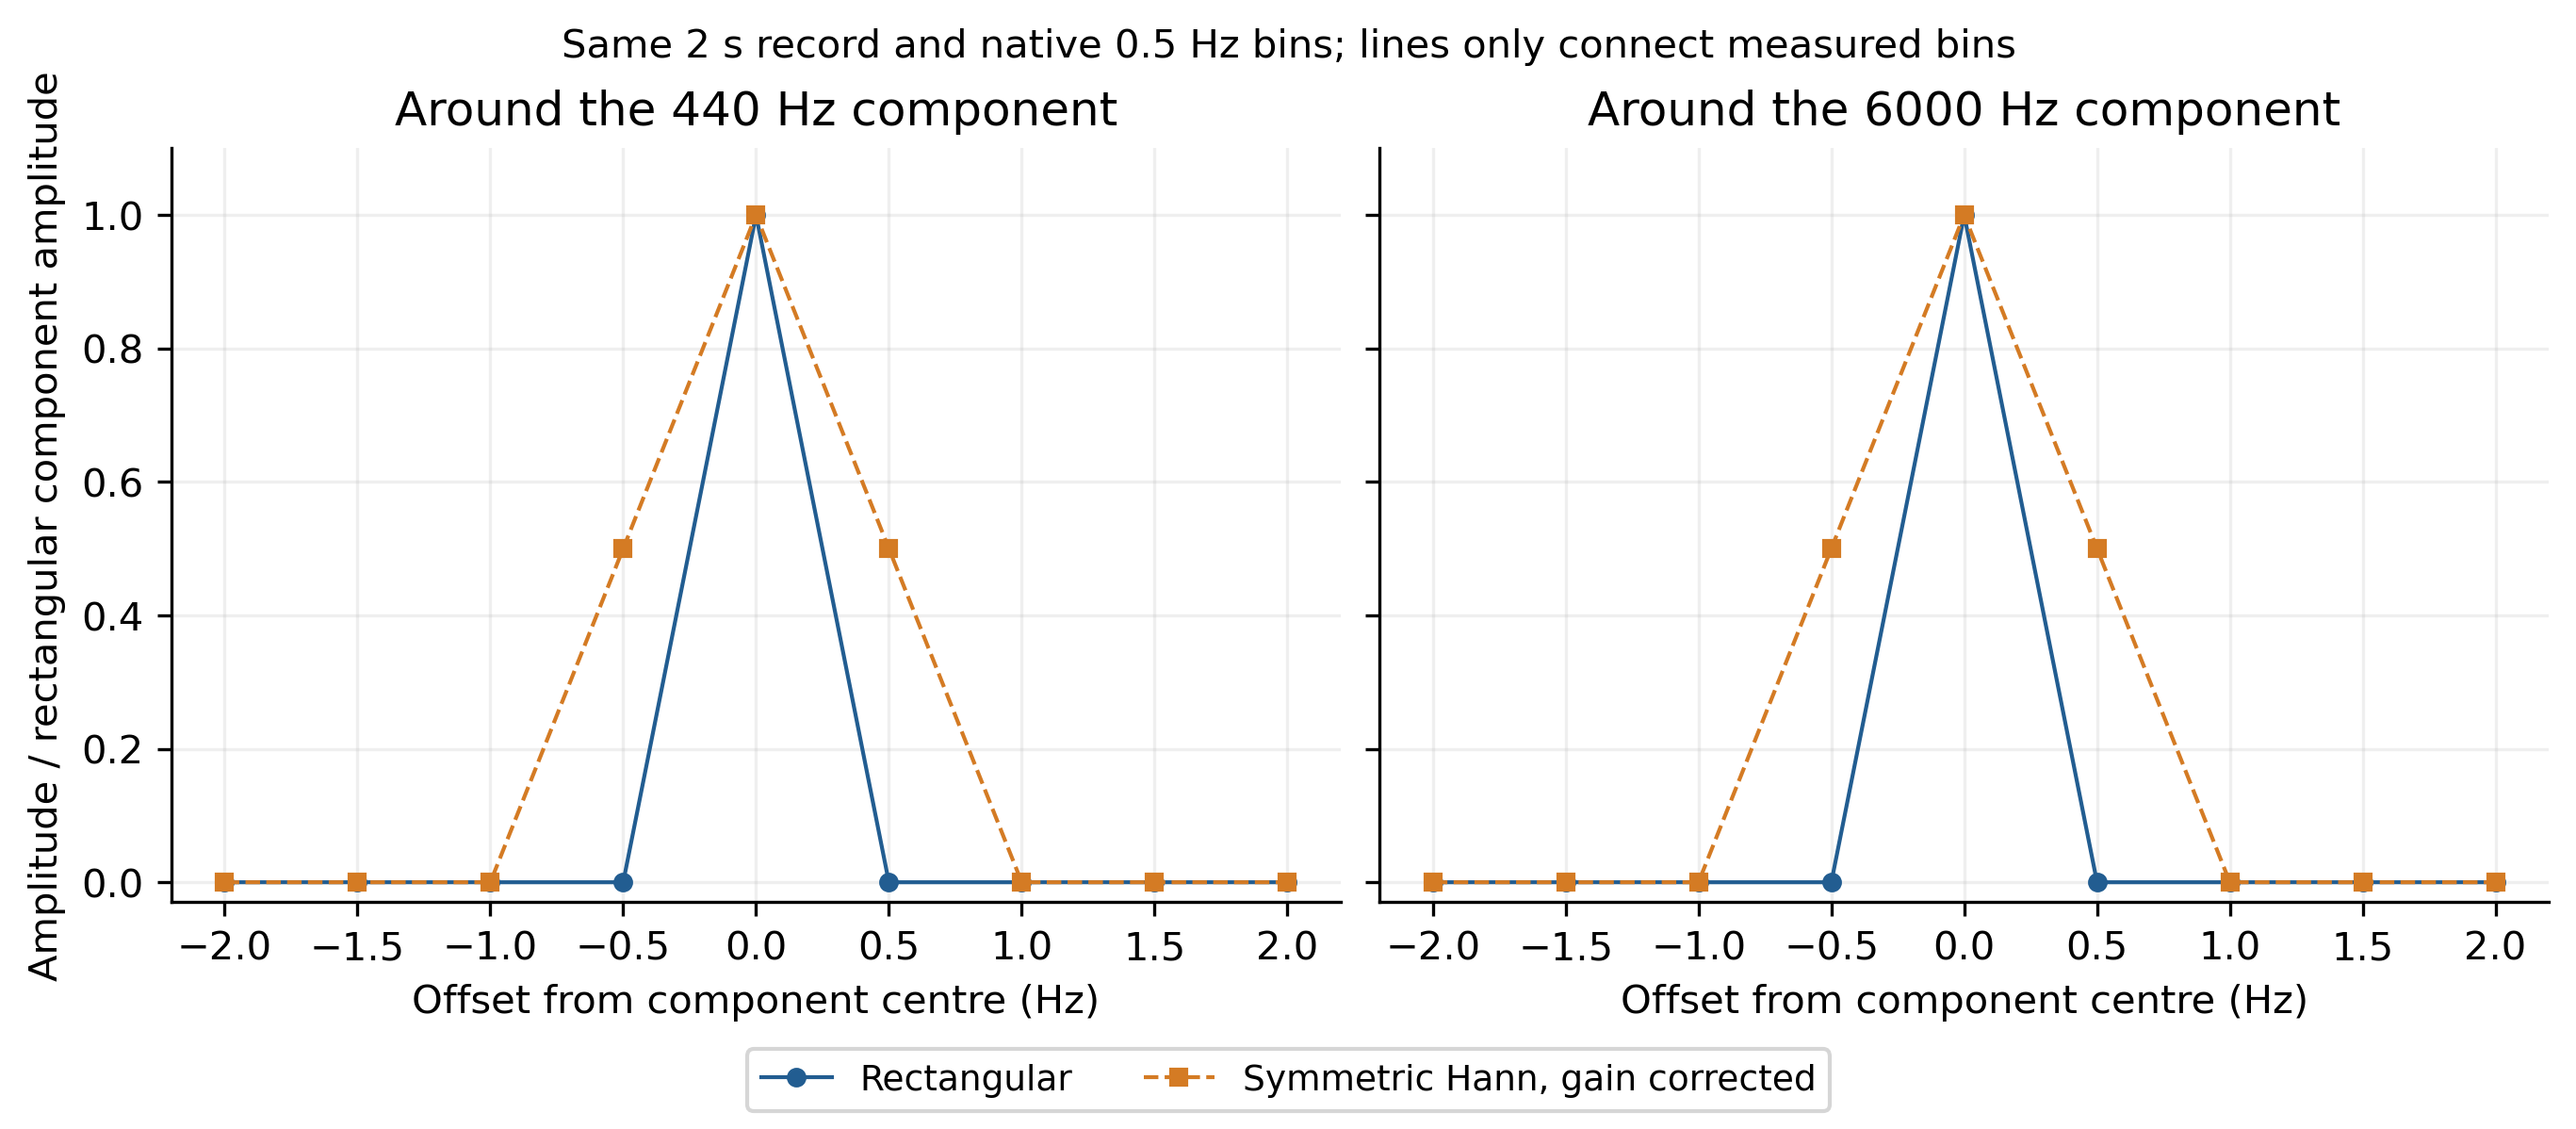
\includegraphics[width=.78\linewidth]{images/window_comparison.png}
 \caption{Same-record window comparison on native 0.5 Hz bins. Hann amplitudes are gain-corrected; adjacent skirts are not additional source tones.}
 \label{fig:window-check}
\end{figure}

The measured tones satisfy $ f_jT\in\mathbb Z $. Hann spreads them into
adjacent bins, including 6000.5 Hz; that bin is not a fifth source tone.
Rectangular therefore retains the narrow coherent peaks here; this choice
does not generalise to noncoherent records. Coherent-gain correction alone
does not remove off-bin or overlapping-tone bias \citep{harris1978windows}.

\paragraph{Define and test bandwidth rather than read a plot by eye.}
\begin{align}
 A_{\mathrm{ref}}&=\max_k\widehat A_R[k],\qquad
 D_w[k]=20\log_{10}\!\left(\frac{\widehat A_w[k]}{A_{\mathrm{ref}}}\right),
 \label{eq:relative-db}\\
 \mathcal K_\theta&=\{k:\ k\text{ is a local maximum and }
 \widehat A_w[k]\ge A_{\mathrm{ref}}10^{\theta/20}\},\qquad\theta=-60\,\mathrm{dB},
 \label{eq:component-detector}\\
 f_B&=\max_{k\in\mathcal K_\theta}f_k=\BandEdgeHz\,\mathrm{Hz}.
 \label{eq:band-edge}
\end{align}
Interior maxima use left-strict/right-nonstrict comparison, with endpoints
tested separately. The operational $-60 $ dB threshold is a project choice;
both windows retain the same four centres at $-40,-60,-80 $ dB. The weakest
tone is about $-20 $ dB. Table~\ref{tab:components} gives measured frequency,
amplitude and power; Figure~\ref{fig:sampling-summary} combines the
full spectrum with the resulting rate decision.

\begin{table}[tbp]
 \centering
 \caption{Measured source components from CSV, in unmodified NPY units. Relative dB uses the largest peak; powers use the paired-coefficient convention.}
 \label{tab:components}
 \begin{tabular}{rrrrr}
\toprule
Bin & Frequency (Hz) & Amplitude & Relative dB & Power (\%) \\
\midrule
880 & 440 & 1.0 & 0.000 & 68.4932 \\
2640 & 1320 & 0.6 & -4.437 & 24.6575 \\
4400 & 2200 & 0.3 & -10.458 & 6.1644 \\
12000 & 6000 & 0.1 & -20.000 & 0.6849 \\
\bottomrule
\end{tabular}

\end{table}

For the alternative cumulative-power definition,
\begin{equation}
 B_q=\min\left\{f_k:\frac{\sum_{i=0}^{k}P_i}{\sum_iP_i}\ge q\right\},
 \label{eq:energy-bandwidth}
\end{equation}
$ B_{0.99}=2200 $ Hz would discard the valid 6 kHz tone, which contributes
0.685 \% of power; $ B_{0.999}=6000 $ Hz retains it. I use the 6 kHz component
edge to preserve every identified tone. This is finite-record evidence,
not strict compact support of its time-truncated DTFT or an unknown
analogue source. Tone powers 0.5, 0.18, 0.045, 0.005 sum to 0.73.
Ten deterministic checks include DC/Nyquist/odd-length scaling, explicit
DFT sums, FFT agreement, inverse, Hann gain and Parseval. Relative
Parseval error is $\ParsevalError $ and maximum same-grid inverse error
is $\RoundTripError $; these checks are distinct from low-rate reconstruction.

\subsection{Choose 16 kHz with a measured cost comparison}
The target is the complete supplied multitone, including its weak highest
component. The reference sampling condition and replica geometry are
 \citep{shannon1949noise}
\begin{equation}
 T_s=1/f_s,\quad x_s[m]=x(mT_s),\quad
 f_s>2f_B=12000\,\mathrm{Hz},\quad f_N=f_s/2.
 \label{eq:rate-condition}
\end{equation}
\begin{equation}
 g=f_s/2-f_B=\SamplingGuard\,\mathrm{Hz},\qquad
 d=f_s-2f_B=2g=\ReplicaGap\,\mathrm{Hz}.
 \label{eq:rate-guard}
\end{equation}
The signal's Nyquist rate is 12 kHz; the selected sampler's Nyquist
frequency is 8 kHz. The 2 kHz guard is a sampling margin, not a measured
filter specification. Following a predict--sample--compare method,
I take actual reference values, not newly generated ideal tones:
\begin{equation}
 x_M[m]=x_{\mathrm{ref}}[Mm],\quad
 f_s=F_0/M,\quad N=L/M,\quad
 t_m=\frac m{f_s}=\frac{Mm}{F_0}.
 \label{eq:integer-sampling}
\end{equation}
$ M=4,3,2,1 $ tests 12, 16, 24, 48 kHz. All records span 2 s and have 0.5 Hz native
spacing. The implementation is \texttt{reference[::factor].copy()}.
The phase-aware folding identity is Eq.~\eqref{eq:decimation-folding};
an independent full-complex-FFT comparison of every bin at five measured
rates differs by at most $\FoldingError $ NPY units.

\begin{table}[H]
 \centering
 \caption{Same 2 s record, common periodic recovery and all 96000 evaluation positions. Raw payload compares equal bits/sample against 16 kHz; 12 kHz is phase-sensitive critical sampling.}
 \label{tab:rates}
 \begin{tabular}{rrrrrr}
\toprule
$f_s$ (kHz) & $M$ & $f_N$ (kHz) & Samples & Raw ratio & MSE \\
\midrule
12 & 4 & 6 & 24,000 & 0.75 & $0.005$ \\
16 & 3 & 8 & 32,000 & 1 & $1.75\times10^{-25}$ \\
24 & 2 & 12 & 48,000 & 1.5 & $1.27\times10^{-25}$ \\
48 & 1 & 24 & 96,000 & 3 & $1.72\times10^{-31}$ \\
\bottomrule
\end{tabular}

\end{table}

Reconstruction uses only low-rate samples and output length, with the
periodic Fourier interpolator of Eq.~\eqref{eq:periodic-interpolation}.
Its $ L/N $ scale and split old-Nyquist term are derived in
Appendix~\ref{app:sampling}. Coherent 2 s periodicity supports this boundary
model. DC/phased-cosine/Nyquist calibrations and SciPy resampling check it
 \citep{scipy1153resample}. Every metric uses all 96000 positions
(Eq.~\eqref{eq:sampling-errors}); no trimming, fitted shift/gain or
reference-assisted recovery is used. At 16 kHz, MSE/NMSE are
$\SamplingMse/\SamplingNmse $, peak error $\SamplingMaxError $.

The 12 kHz boundary loses the 6 kHz sine through its measured phase near
$-\pi/2 $ (Eq.~\eqref{eq:critical-phase}): endpoint amplitude
$\CriticalToneAmplitude $, MSE $\CriticalMse $, agreeing with the missing
tone power 0.005. Higher 24/48 kHz rates have numerical-residual errors too,
but require more payload. Since $48000/M>12000 $ implies $ M<4 $,
16 kHz is the lowest sufficient tested integer-decimation choice;
it saves one third/two thirds of 24/48 kHz raw bits at fixed $ B $
(Eq.~\eqref{eq:sampling-payload}). The theoretically valid 14.4 kHz
alternative would save 10 \% relative to 16 kHz with 1.2 kHz guard, but needs
noninteger resampling, which I have not measured. I accept 11.11 \% extra
payload relative to it for direct indexing and a larger guard.
This is not a global optimum under later noise.

No appreciable source components lie beyond 6 kHz, so no extra prefilter
is inserted in this clean index-selection study. An arbitrary broadband
input would require anti-alias filtering. The specified noise is added
after downsampling and cannot alias through that earlier operation.
Twelve calibration/grid/phase/error checks pass; R1 is deterministic.

\subsection{Deliberate undersampling and recovery}
The controlled failure bypasses anti-alias filtering at 8 kHz, against
the selected 16 kHz path. Removing 6 kHz before sampling would test content
loss instead of folding. No stochastic degradation or quantisation is used.
\begin{equation}
 x_{16}[m]=x_{\mathrm{ref}}[3m],\qquad
 x_8[m]=x_{\mathrm{ref}}[6m].
 \label{eq:r13-samples}
\end{equation}
Both last 2 s, with 0.5 Hz bin spacing. The mathematical prediction precedes
sample/spectrum checks:
\begin{equation}
 f_d=f_0-qf_s\in[-f_s/2,f_s/2),\qquad f_a=|f_d|,
 \label{eq:signed-alias}
\end{equation}
The implementation is $ f_d=((f_0+f_s/2)\bmod f_s)-f_s/2 $.
At 8 kHz, 6000 Hz maps to $-2000 $ Hz; its positive 2 kHz cosine phase changes
from $-\pi/2 $ to $+\pi/2 $ (Eq.~\eqref{eq:alias-phase}). The 440/1320/2200 Hz
tones remain distinct, with no collisions or endpoint ambiguities.

\begin{table}[!htbp]
 \centering
 \caption{Predicted/detected 8 kHz peaks; phase is in units of $\pi $. The 6 kHz source folds to positive 2 kHz with reversed cosine phase.}
 \label{tab:alias-mapping}
 \begin{tabular}{rrrrrr}
\toprule
Source (Hz) & Signed (Hz) & Predicted (Hz) & Measured (Hz) & Amplitude & $\phi/\pi$ \\
\midrule
440 & 440 & 440 & 440 & 1.0 & -0.500 \\
1320 & 1320 & 1320 & 1320 & 0.6 & -0.500 \\
2200 & 2200 & 2200 & 2200 & 0.3 & -0.500 \\
6000 & -2000 & 2000 & 2000 & 0.1 & 0.500 \\
\bottomrule
\end{tabular}

\end{table}

% Keep the measured-peak result paragraph intact across the table/figure stack.
\noindent\begin{minipage}{\linewidth}
Peaks are detected with the same $-60 $ dB local-maximum rule, rather than
declared measured by selecting predicted bins. Normalised complex
coefficients and wrapped phases are also checked; all 16 checks pass.
Both paths use the same Fourier recovery and all original grid positions.
The 8 kHz MSE/RMSE/NMSE/peak error are $\UnderMse $, $\UnderRmse $,
$\UnderNmse $ and $\UnderMaxError $; the 16 kHz MSE is $\AliasBaselineMse $.
\end{minipage}\par

\begin{figure}[!htbp]
 \centering
 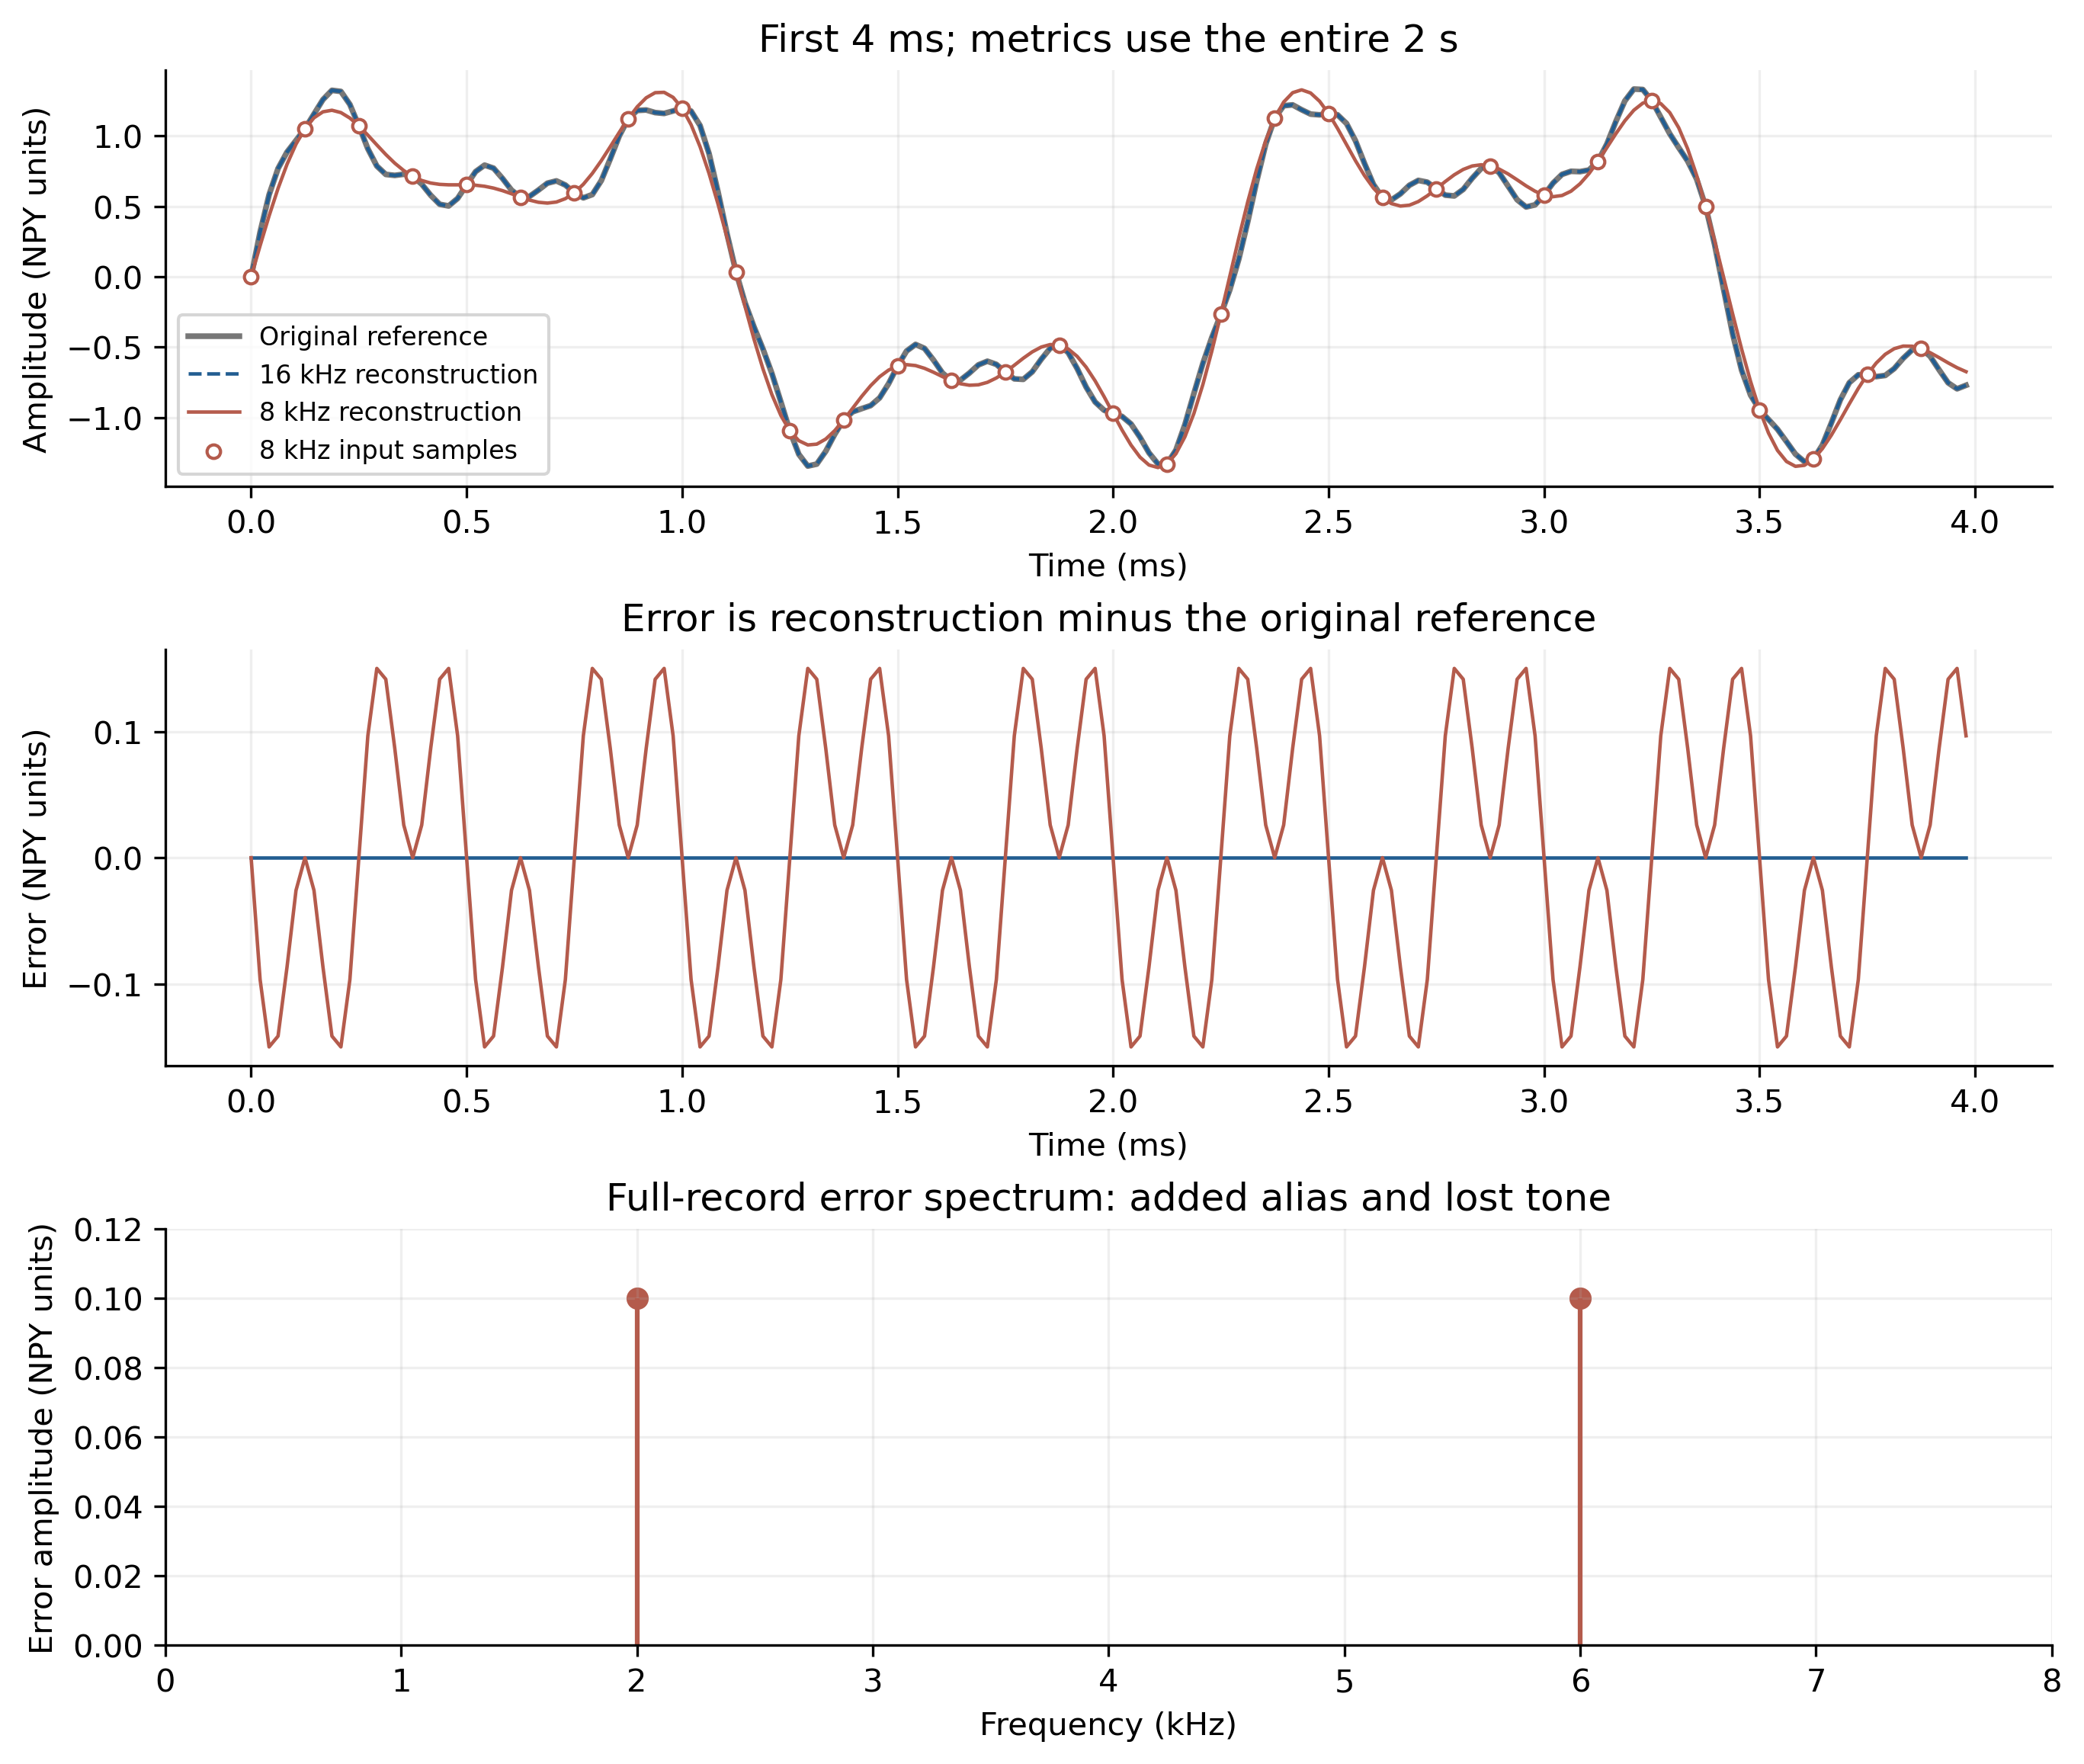
\includegraphics[width=.76\linewidth]{images/aliasing_reconstruction_error.png}
 \caption{Recovery and error: first 4 ms waveforms above, full 2 s error spectrum below. All 96000 positions enter the reported MSE; sample fitting alone does not identify the source.}
 \label{fig:alias-recovery}
\end{figure}

% Keep this result paragraph together if the preceding figure moves to a page top.
\noindent\begin{minipage}{\linewidth}
Both recoveries fit their own samples to about $10^{-15}$, demonstrating
that sample fitting does not identify the source. The phase-aware error
model predicts 0.1-amplitude tones at 2/6 kHz and MSE 0.01
(Eqs.~\eqref{eq:alias-error-model}--\eqref{eq:alias-error-power}); the
full-record error spectrum agrees. This explanation is not information
supplied to recovery. Complex coefficients must be added before power
when aliases coincide. Later filtering/coding cannot resolve this
ambiguity without extra source information.
\end{minipage}\par

\subsection{Integrated sampling decision}
\begin{equation}
 \boxed{f_B=\BandEdgeHz\,\mathrm{Hz}
 \ \Longrightarrow\ f_s>2f_B=12000\,\mathrm{Hz}
 \ \xrightarrow{\ f_s=F_0/M,\ M=3\ }\ f_s=\TransmissionRate\,\mathrm{Hz}.}
 \label{eq:decision-chain}
\end{equation}
The last arrow is a design choice: the measured 6 kHz edge, tested
16 kHz recovery and 12/8 kHz failure evidence justify it, with the payload
and untested-alternative costs stated above.

\begin{figure}[!htbp]
 \centering
 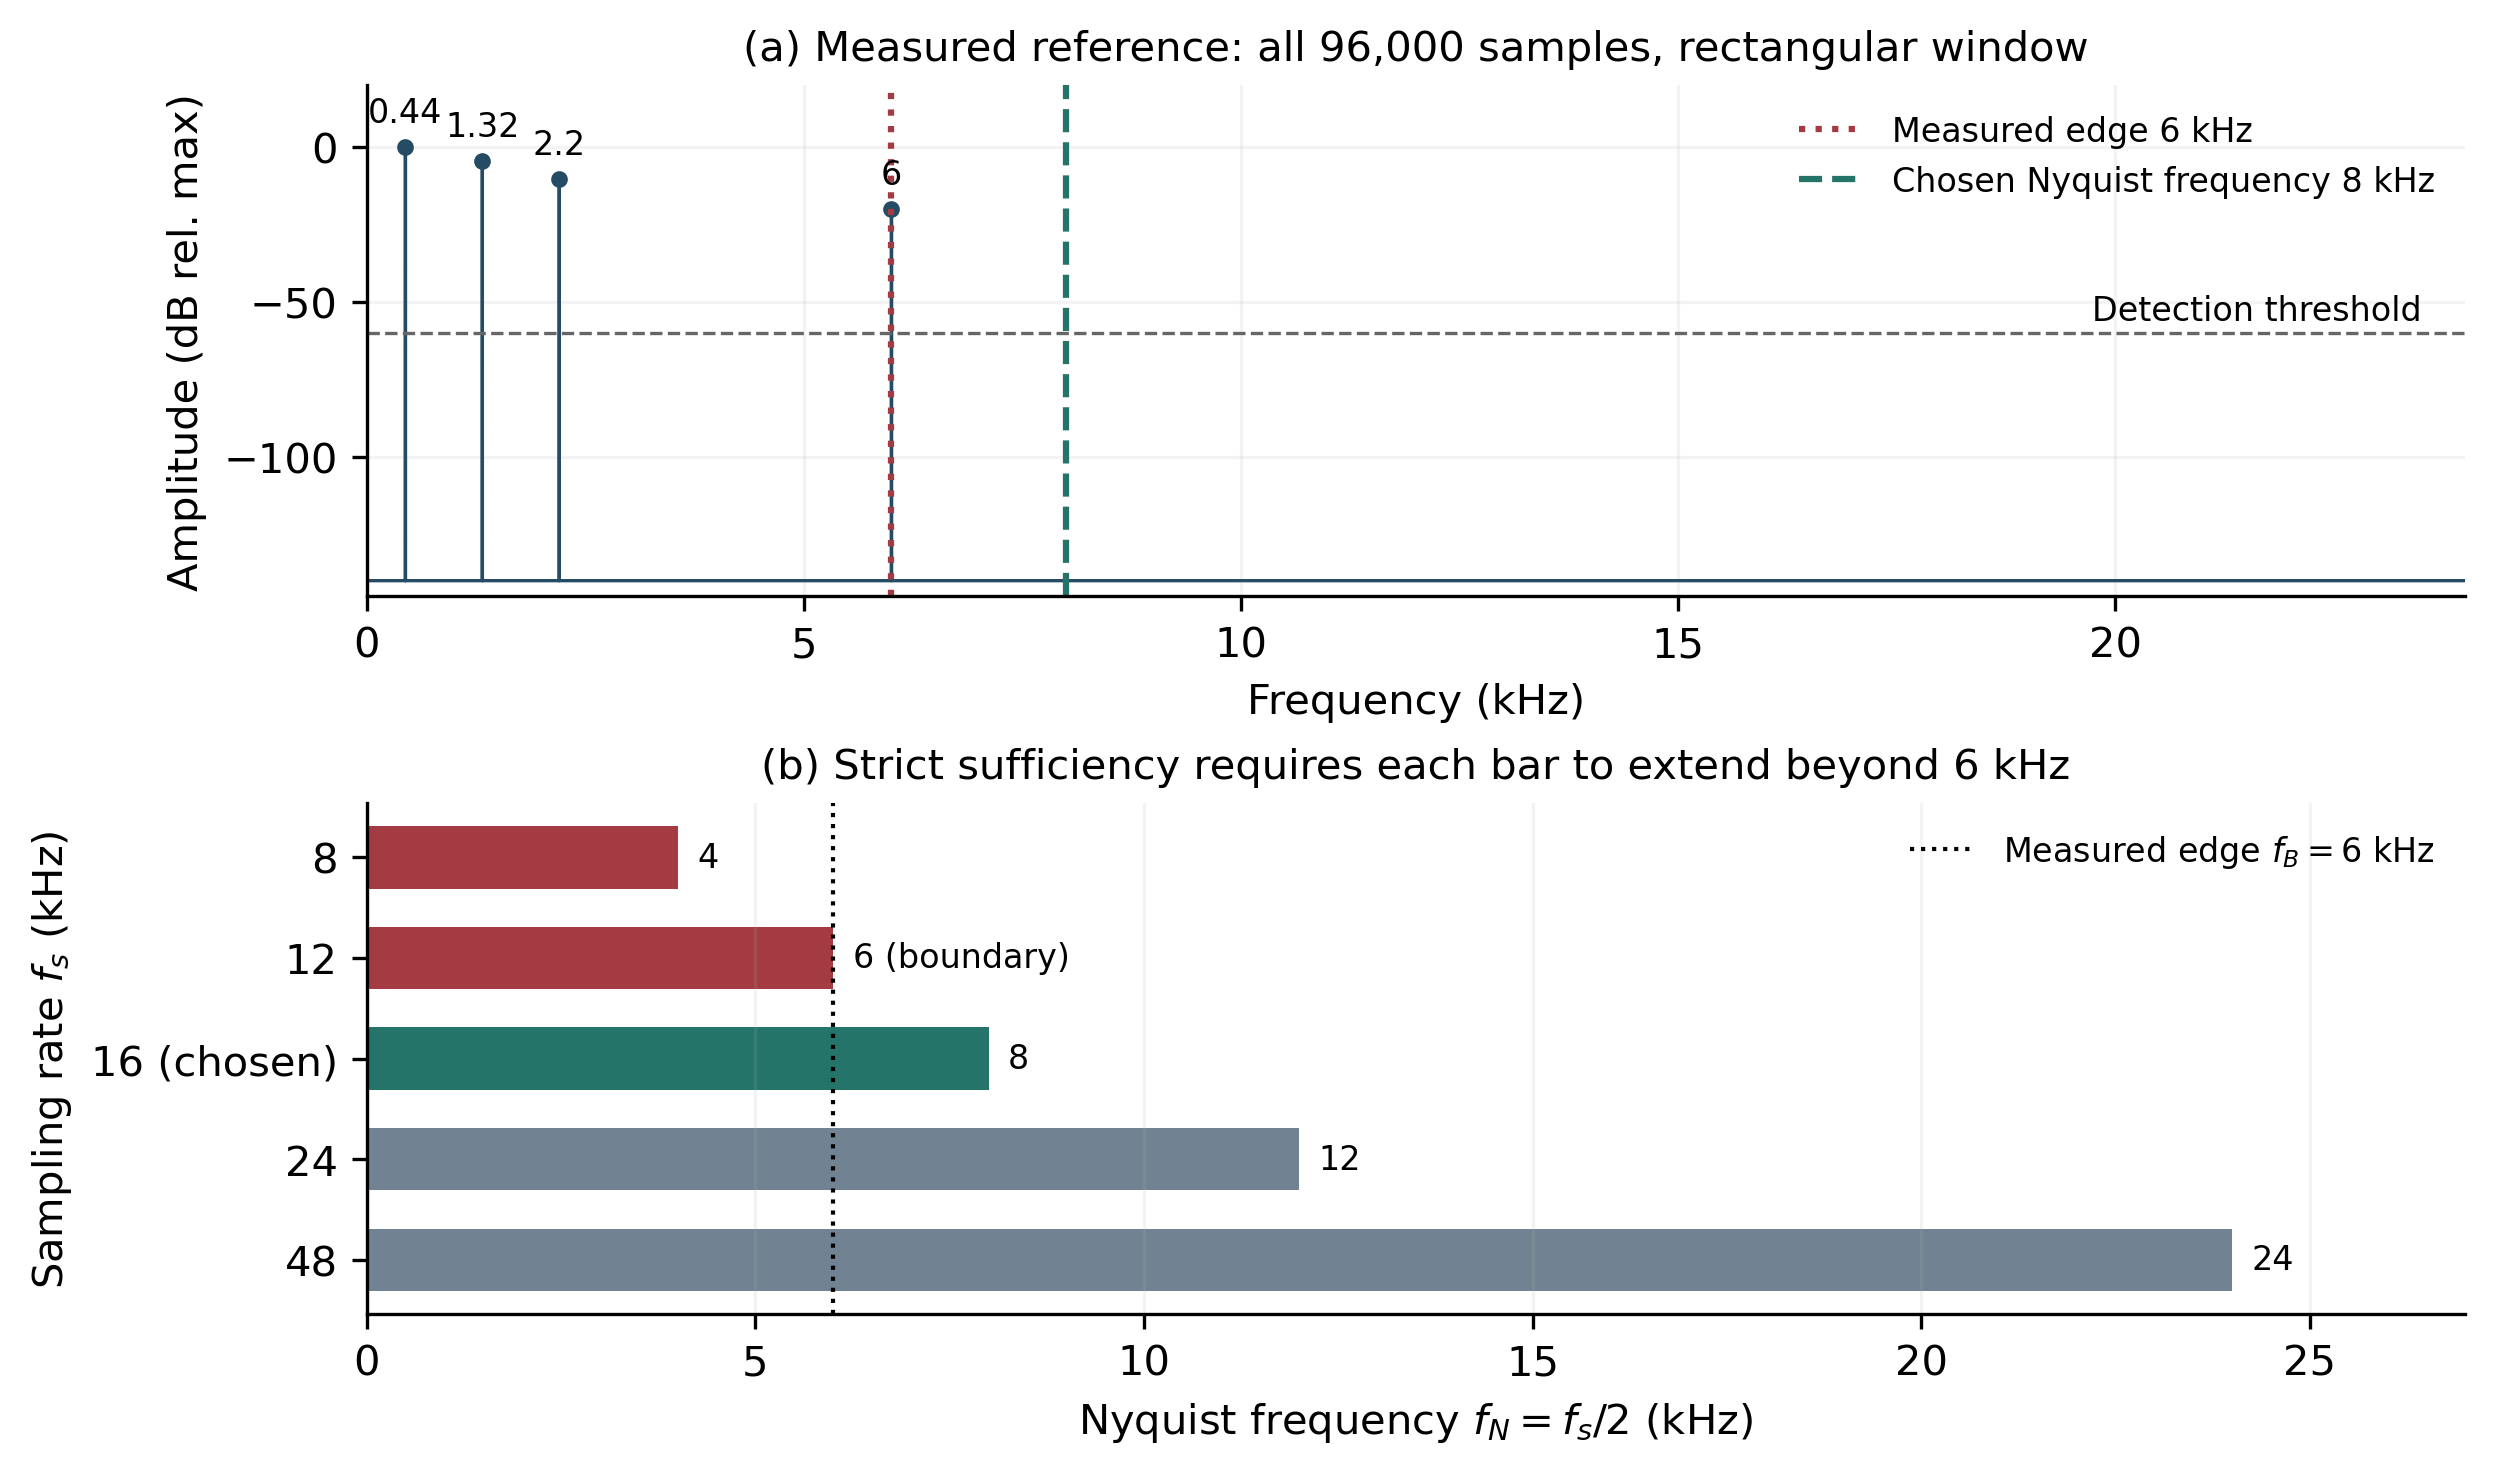
\includegraphics[width=.76\linewidth]{images/sampling_decision.png}
 \caption{Integrated R1 evidence: full-reference spectrum and candidate Nyquist limits. Peak labels use kHz; the $-60 $ dB detector and $-140 $ dB display floor have separate roles. The selected sampler leaves a 2 kHz guard.}
 \label{fig:sampling-summary}
\end{figure}

\path{stage1/r14/results/decision_summary.csv} joins
the five existing rates; six cross-stage checks and seven input hashes
verify this reporting join, which introduces no new measurements.

\FloatBarrier
\section{Stage 2: Filtering}
\subsection{Choose a multiband FIR implemented by FFT convolution}
\label{sec:r21}
I select a multiband FIR because four tones leave wide noise-only gaps.
FFT convolution gives the direct-convolution result efficiently; denoising
comes from the filter, not the FFT. The implementation follows linear
convolution and Fourier analysis;
Appendix~\ref{app:filter} derives padding and the centre crop.
For the 513-tap prototype, $K\ge N+M-1=32512$; $K=32768$ is convenient,
not mandatory, before cropping to 32000. Padding, identity and zero-filter
controls check this implementation.

The input is exactly $ u[3n]$ with measured power 0.73. Gaussian degradation
follows Eq.~\eqref{eq:noise-contract} after sampling. I declare the
anchor-SNR range $[0,30]$ dB (equal signal/noise power down to one
thousandth). Parameter leaf $(0,0)$ gives
\begin{equation}
 U_S=\RtwoUniform,\qquad
 S_0=0+(30-0)U_S=\RtwoPersonalSnr\ {\rm dB}.
 \label{eq:r21-personal-snr}
\end{equation}
Three phase-0 draws at $-10,0,10,20,30,S_0 $ give 18 paired design records,
noise paths $(1,2,0,c,r)$. All methods share each contaminated array.
Personal repeat 0 realises $\RtwoRealisedSnr $ dB; draws are not rescaled.
Searching its spectrum within $\pm10 $ Hz of declared R1 priors recovers
440/1320/2200/6000 Hz. This is informed design, not blind discovery;
the true noise vector never enters construction.

The three-point mean has aligned response $(1+2\cos\omega)/3 $.
At 6 kHz it is $(1-\sqrt2)/3=-0.138071 $, attenuating and reversing a valid
tone; clean-input MSE is $\RtwoMaClean $. A broad low-pass also retains
much white noise. The prototype instead uses an even four-band
$\pm80 $ Hz template, a 513-tap IDFT crop and a symmetric Hann kernel
taper; a 6600 Hz low-pass is the matched construction comparator.
This taper acts on coefficients, not the input record.

\begin{table}[!htbp]
 \centering\small
 \caption{Method-selection pilot: three paired design draws per level, all 32000 samples. Prototype parameters are provisional; these are design results.}
 \label{tab:r21-pilot}
 \begin{tabular}{rrrrr}
\toprule
Input SNR (dB) & No filter & Three-point mean & Wide low-pass & Multiband \\
\midrule
-10 & $7.2808\times10^{0}$ & $2.4291\times10^{0}$ & $5.9946\times10^{0}$ & $5.0234\times10^{-1}$ \\
0 & $7.2922\times10^{-1}$ & $2.5037\times10^{-1}$ & $6.0001\times10^{-1}$ & $4.9542\times10^{-2}$ \\
10 & $7.2617\times10^{-2}$ & $3.4625\times10^{-2}$ & $5.9907\times10^{-2}$ & $5.1871\times10^{-3}$ \\
20 & $7.3307\times10^{-3}$ & $1.2779\times10^{-2}$ & $6.0115\times10^{-3}$ & $6.7432\times10^{-4}$ \\
30 & $7.3223\times10^{-4}$ & $1.0605\times10^{-2}$ & $6.0365\times10^{-4}$ & $2.5071\times10^{-4}$ \\
\bottomrule
\end{tabular}

\end{table}

The multiband clean MSE is $\RtwoMultiClean$; fixed 256-sample
edges/interior give $\RtwoMultiEdge/\RtwoMultiInterior$, both retained.
Its offline prototype has 16 ms causal group delay, not total latency.
Direct/FFT outputs agree over 18 inputs within $\RtwoFftError$;
all $\RtwoCheckCount$ checks pass. The reference costs are
$O(NM)$ versus $O(K\log K)$ \citep{duhamel1990fft}, without a measured runtime claim.
This pilot selects the family; R2.2 tunes its distortion/noise tradeoff,
and R2.3 evaluates unused noise.

\subsection{Choose, justify and freeze the filter parameters}
\label{sec:r22}
I freeze $\RttLength $ symmetric \RttWindow{} taps, nominal half-width
$\RttHalfWidth $ Hz, delay $\RttDelay $ samples ($\RttDelayMs $ ms) and
$K=\RttFFT$, using the measured spectrum and rule below.

\paragraph{Corrupted-spectrum evidence.}
Spectral analysis of anchor phase-0 repeat 0 uses rectangular, symmetric
Hann and Hamming observation windows, distinct from FIR tapers. Equations~\eqref{eq:r22-spectrum-scales}
and \eqref{eq:r22-psd-integral} set amplitude/PSD scales and Parseval.
Native PSD uses $K=N$; literal $-3.000$ dB amplitude widths use 16-fold
padding and interpolated crossings:
\begin{align}
 \widehat S_{\rm bg}&=\frac1{|\mathcal B|}
       \sum_{k\in\mathcal B}\widehat S_{{\rm rect},N}[k],&
 L_i&=10\log_{10}\frac{\widehat S_{{\rm rect},N}[k_i]}
                            {\widehat S_{\rm bg}},\nonumber\\
 A_{\rm threshold}&=A_{\rm local\,peak}10^{-3/20},&
 W_{-3{\rm dB}}&=f_R-f_L.
 \label{eq:r22-spectrum-measures}
\end{align}
$\mathcal B $ comprises interior positive bins outside $\pm20 $ Hz of
the four priors. The mean off-band PSD is $\RttPsdBackground $ squared
NPY units/Hz; the 6 kHz peak lies $\RttWeakPeakBackground $ dB above it.
Padding refines the grid to 0.03125 Hz, not the 0.5 Hz native resolution;
power/amplitude ratios use 10/20 log, respectively.

\begin{table}[!htbp]
 \centering\small
 \caption{Corrupted-spectrum evidence. Analysis-peak widths are Hz, distinct from FIR passbands; peak/background uses native rectangular PSD.}
 \label{tab:r22-spectrum}
 \begin{tabular}{rrrrr}
\toprule
Centre (Hz) & Peak/background (dB) & Rect. width & Hann width & Hamming width \\
\midrule
440 & 43.00 & 0.4414 & 0.7185 & 0.6496 \\
1320 & 38.71 & 0.4400 & 0.7103 & 0.6432 \\
2200 & 32.68 & 0.4432 & 0.7240 & 0.6546 \\
6000 & 23.46 & 0.4353 & 0.7207 & 0.6475 \\
\bottomrule
\end{tabular}

\end{table}


\begin{figure}[!htbp]
 \centering
 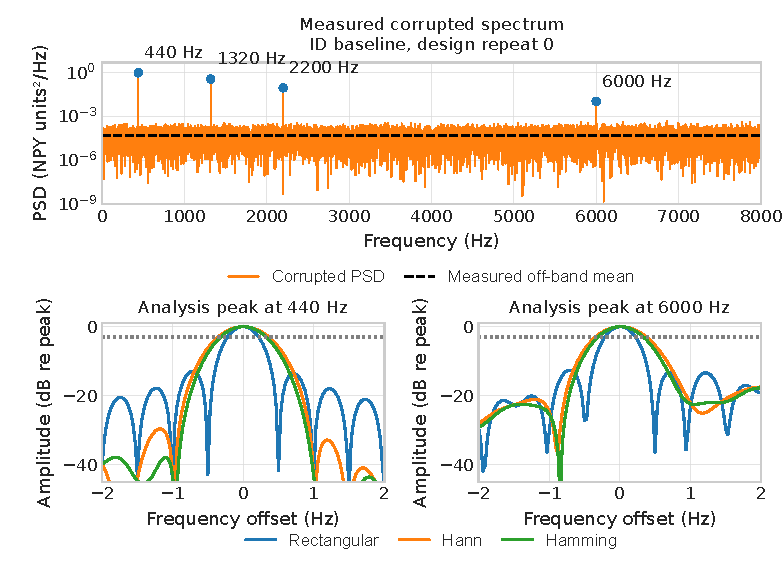
\includegraphics[width=.82\linewidth]{supporting/publication_r22_corrupted_spectral_evidence.pdf}
 \caption{Personal phase-0 spectrum: native PSD/background above; three observation-window peaks and interpolated $-3.000$ dB widths below.}
 \label{fig:r22-corrupted-evidence}
\end{figure}

Sub-hertz observation widths support separated bands; finite-FIR
passbands also depend on truncation, gain and boundaries.
\paragraph{Measured search with explicit constraints.}
The project-designed kernel uses the reference window formulas in
Eqs.~\eqref{eq:r22-family} and \eqref{eq:r22-windows}.
Six lengths 129/257/513/1025/2049/4097, seven half-widths
2/5/10/20/40/80/160 Hz and three tapers give 126 coarse candidates.
Require positive aligned gain within 1\% over centre $\pm2$ Hz,
checked every 0.5 Hz:
\begin{equation}
 G(f)=\sum_{m=0}^{M-1}h[m]e^{-j2\pi f(m-d)/f_s},\qquad
 \bigl||G(f_i+\delta)|-1\bigr|\le0.01.
 \label{eq:r22-gain-constraint}
\end{equation}
The guard is a design allowance, not measured drift. All candidates share
18 design records; selection uses $\mathcal C=\{0,10,20,30,S_0\}$ dB,
$R=3$, and the balanced score
\begin{equation}
 J=\frac1{|\mathcal C|R}\sum_{c\in\mathcal C}\sum_{r=0}^{R-1}
 \frac{\mathrm{MSE}_{\rm out}(c,r)}{\mathrm{MSE}_{\rm in}(c,r)}.
 \label{eq:r22-objective}
\end{equation}
Each MSE includes 32000 samples; paired normalisation balances SNRs.
The $-10$ dB stress point is excluded. Reference-based scoring supplies no
truth to recovery. Refining adjacent bounds around the feasible minimum
uses seven odd lengths and 13 widths rounded to 0.5 Hz; with coarse
points, $\RttCount$ candidates include $\RttFeasible$ feasible choices.
Within 1\% of minimum $J$, prefer shortest length, then lower $J$,
narrower band and registered window order. The winner is also the strict
tested minimum and is unchanged at 0/0.5/1\% allowances.

\begin{figure}[!htbp]
 \centering
 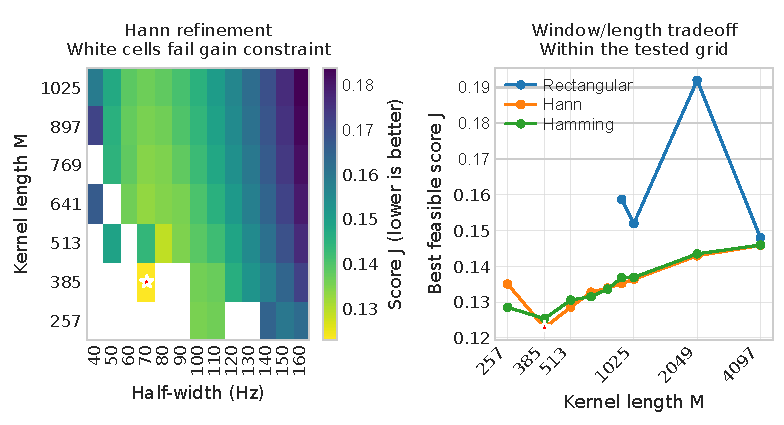
\includegraphics[width=.82\linewidth]{supporting/publication_r22_parameter_search.pdf}
 \caption{Hann refinement (white: gain-guard failure) and each taper's best feasible tested width at each length. Star: frozen 385-tap choice.}
 \label{fig:r22-search}
\end{figure}


\begin{table}[!htbp]
 \centering\small
 \caption{Best feasible tested candidate per kernel taper. Scores use the same declared paired design objective, not a universal window ranking.}
 \label{tab:r22-windows}
 \begin{tabular}{lrrrr}
\toprule
Kernel window & $M$ & Half-width (Hz) & $J$ & Clean-input MSE \\
\midrule
Rectangular & 4097 & 80 & 0.147986 & $2.2352\times10^{-4}$ \\
Hann & 385 & 70 & 0.122854 & $2.2951\times10^{-4}$ \\
Hamming & 385 & 70 & 0.125388 & $2.3551\times10^{-4}$ \\
\bottomrule
\end{tabular}

\end{table}

\paragraph{Result, reason and cost.}
The four nominal positive bands are
 $[370,510]$, $[1250,1390]$, $[2130,2270]$ and $[5930,6070]$
 Hz, plus conjugate negative bands.
Realised $-3 $ dB full widths are about $\RttBandWidthMin $ Hz; they are not
the 140 Hz template widths. Maximum guard gain deviation is
$\RttGainPercent $\%. Relative to the 513-tap prototype, score falls from
$\RttOldScore $ to $\RttScore $ ($\RttScoreImprovement $\%), and group delay
from 16 to 12 ms. Both use the same FFT length; runtime gain is unmeasured.
Whole-record buffering is 2 s, so group delay is not total latency. Clean MSE rises to $\RttCleanMse $,
while finite-record noise gain falls to $\RttNoiseGain $; at 30 dB design
MSE $\RttHighNew $ exceeds the prototype's $\RttHighOld $.

\begin{figure}[!htbp]
 \centering
 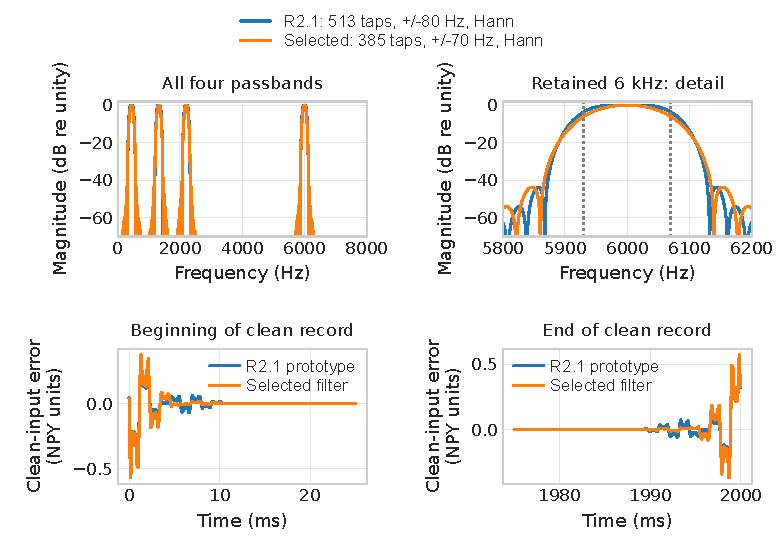
\includegraphics[width=.82\linewidth]{supporting/publication_r22_response_boundary.pdf}
 \caption{Realised FIR response and retained clean-input endpoint distortion. Template edges and measured $-3.000$ dB widths differ.}
 \label{fig:r22-response-boundary}
\end{figure}

The fixed-filter expectation $ D+\sigma^2G_{\rm finite}$ predicts a
sample-grid crossover near $\RttCrossover $ dB (Appendix~\ref{app:filter});
every trial retains its cross term. Ten checks cover PSD, IDFT,
convolution, symmetry and finite-boundary gain. Coefficients/hashes in
\path{stage2/r22/results/filter_freeze.json} precede phase 1.

\subsection{Independent recovery assessment and failure boundary}
\label{sec:r23}
The frozen 385-tap FIR $ F $ and bypass receive the identical $ y=x+e $.
With the unchanged periodic recovery $ R $,
\begin{equation}
 z_0=y,\quad z_F=F(y),\qquad
 \widehat x_0=R(y),\quad \widehat x_F=R(F(y)).
 \label{eq:r23-branches}
\end{equation}
All 96000 reconstructed positions enter MSE/NMSE; no fitted gain, shift
or trimmed endpoint is allowed. Eq.~\eqref{eq:r23-metrics} gives units;
Eq.~\eqref{eq:r23-paired} gives paired reduction and error-SNR gain.
The mean gain averages individual logarithmic gains, not the logarithm
of mean MSEs. Error SNR includes deterministic distortion and differs
from target Gaussian SNR. The signal/error-power approach supports
this metric; correlation alone would
give one for $\widehat u=2u $ despite MSE $ P_u $.

Before drawing phase-1 noise I fix 50 complete records at each of
$-10,0,S_0,10,20,30,35,40 $ dB: 400 records, paths $(1,2,1,c,r)$.
The 35/40 dB diagnostics probe the predicted crossover without changing
the declared personal range. Whole records are independent; filtered
positions are not extra replicates. Mean intervals use the common
approximate t/CLT rule with $ R=50,m=1 $
(Appendix~\ref{app:statistics}; \citealp{scipy1153t,scipy1153sem}).
These pointwise mean intervals are neither simultaneous nor predictions
for a new record; count 50 makes no predeclared precision guarantee.

\begin{table}[!htbp]
 \centering
 \caption{Independent validation, 50 paired records per condition on all 96000 positions. Pointwise approximate 95 \% intervals describe mean gain; the dagger marks the personal baseline.}
 \label{tab:r23-quality}
 \footnotesize\setlength{\tabcolsep}{4pt}
 \begin{tabular}{rrrrr}
\toprule
Target $S$ & Mean MSE, no filter & Mean MSE, filter & Mean gain [95\% CI] & Wins \\
(dB) & (NPY units$^2$) & (NPY units$^2$) & (dB) & (/50) \\
\midrule
-10 & $7.2955\times10^{0}$ & $3.8900\times10^{-1}$ & 12.733 [12.703, 12.762] & 50 \\
0 & $7.3081\times10^{-1}$ & $3.8987\times10^{-2}$ & 12.730 [12.695, 12.766] & 50 \\
2.661$^\dagger$ & $3.9576\times10^{-1}$ & $2.1209\times10^{-2}$ & 12.711 [12.678, 12.743] & 50 \\
10 & $7.3101\times10^{-2}$ & $4.1467\times10^{-3}$ & 12.464 [12.431, 12.496] & 50 \\
20 & $7.3015\times10^{-3}$ & $6.1966\times10^{-4}$ & 10.714 [10.685, 10.743] & 50 \\
30 & $7.3097\times10^{-4}$ & $2.6878\times10^{-4}$ & 4.345 [4.329, 4.361] & 50 \\
35 & $2.3069\times10^{-4}$ & $2.4202\times10^{-4}$ & -0.208 [-0.219, -0.198] & 0 \\
40 & $7.2974\times10^{-5}$ & $2.3326\times10^{-4}$ & -5.047 [-5.055, -5.038] & 0 \\
\bottomrule
\end{tabular}

\end{table}


\begin{figure}[!htbp]
 \centering
 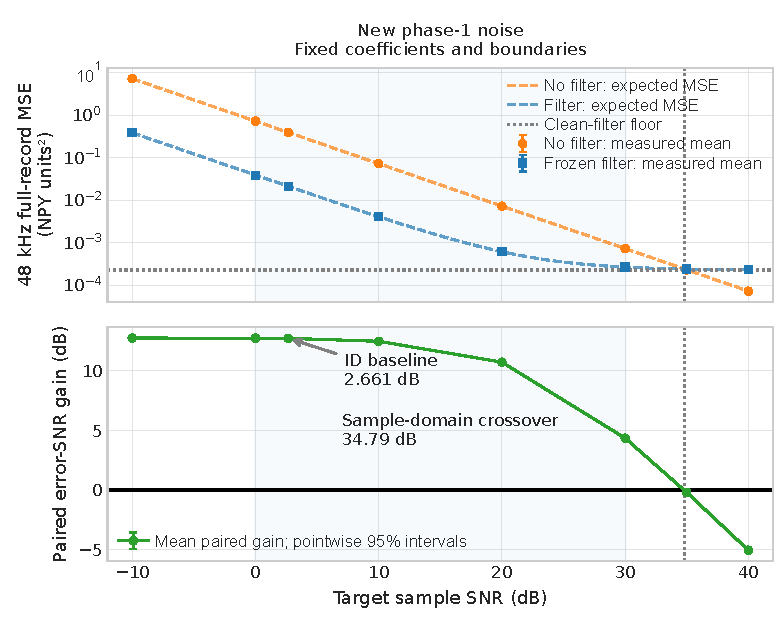
\includegraphics[width=.82\linewidth]{supporting/publication_r23_recovery_quality.pdf}
 \caption{Held-out mean MSE versus prediction (top) and paired gains with pointwise intervals (bottom). Shading: design range; line: prevalidation crossover.}
 \label{fig:r23-quality}
\end{figure}

\begin{samepage}
At the anchor point mean MSE falls from $\RtvPersonalBefore $ to
$\RtvPersonalAfter $ ($\RtvPersonalReduction $\%); mean paired gain is
$\RtvPersonalGain $ dB, interval $[\RtvPersonalLow,\RtvPersonalHigh]$.
All 50 improve at every tested level through 30 dB, including $-10 $ dB;
all 50 worsen at 35 and 40 dB. This is evidence at tested conditions,
not every realisation or every intermediate SNR. Fixed FIR distortion
persists after the input noise diminishes.
\end{samepage}

Prediction on the 48 kHz grid includes the old-Nyquist splitting correction
(Eq.~\eqref{eq:r23-reconstruction-energy}); sample-grid and recovered
powers are not silently equated. The no-filter gain is 0.999984375;
filtered gain $\RtvNoiseGainHigh $ and distortion $\RtvCleanHigh $ give
the plotted $ D_{48}+\sigma^2G_{48}$ prediction. At 40 dB, the first/last
768 positions, only 1.6 \% of duration, contribute
$\RtvHighEdgePercent $\% of filtered squared error. Edge shares use
aggregated sums, not averaged per-record ratios
(Eq.~\eqref{eq:r23-boundary-metrics}); they remain in every primary MSE.

Twelve checks cover inputs, freezing, disjoint seeds, grids and identities.
Twenty further audit checks use the separate cosine-series kernel
(Eq.~\eqref{eq:r23-audit-kernel}) and $K=64000$ real FFT to reproduce
372 scores/6696 design MSEs; the alternative-method replay in
Section~\ref{sec:r61} also checks all 400 validation inputs.
Records are in \path{metadata/r2_strict_checks.csv} and
\path{stage2/r23/results/}; these are replays, not extra data or retuning.

\FloatBarrier
\section{Stage 3: Quantisation and error control}
Phase-0 measurements select the quantiser and code; a separate phase-1
study validates the frozen choices. All results use the supplied signal,
the R2 FIR and the receiver in Figure~\ref{fig:system-flow}.
\subsection{Resolution from measured SQNR and fidelity}
\label{sec:r31}
I select $ B=\QBits $, $ A=\QHalfRange $ and $\QLevels $ endpoint levels.
The endpoint scale--round--inverse mapping, extended by fixed scaling
and saturation, is 
\begin{align}
 z_c[n]&=\operatorname{clip}(z[n],-A,A),&
 v[n]&=z_c[n]/A,\qquad L=2^B,\\
 j[n]&=\operatorname{clip}\!\left(
 \operatorname{round}\!\left[\frac{v[n]+1-\epsilon}{2}(L-1)\right],
 0,L-1\right),\\
 z_q[n]&=A\left(\frac{2j[n]}{L-1}-1\right),
 \label{eq:r31mapping}\\
 q_j&=-A+\frac{2Aj}{L-1},&
 \Delta&=q_{j+1}-q_j=\frac{2A}{L-1}.
 \label{eq:r31spacing}
\end{align}
The implemented spacing is $2A/(2^B-1)$, whereas standard analysis uses
$\Delta_{\rm lec}=2A/2^B $.
I retain the fixed $\epsilon=10^{-9}$ and NumPy round-to-even.
The shifted granular bound is $|z_q-z_c|\le\Delta/2+A\epsilon $;
zero maps to $-\Delta/2 $, so exact zero bias is not assumed.
Appendix~\ref{app:quant} derives the codebook, headroom and error model.

The original signal already exceeds $[-1,1]$. Before drawing noise I fix
the same $ A=18 $ for filtered and unfiltered inputs over the declared
$-10 $ to 40 dB envelope. Six-standard-deviation headroom gives paired-record
overload bound $\QUnionBound $; it cannot guarantee no overload for an
unbounded Gaussian. Overloads are counted before clipping; none occurred
in the 80 branch records.
The measured implemented error-power ratio is
\begin{align}
 e_q[n]&=z_q[n]-z[n],\\
 P_z=\frac1N\sum_{n=0}^{N-1}z[n]^2,\qquad
 P_{e_q}&=\frac1N\sum_{n=0}^{N-1}e_q[n]^2,\\
 {\rm SQNR}_{\rm meas}&=10\log_{10}\frac{P_z}{P_{e_q}}.
 \label{eq:r31sqnr}
\end{align}
The uniform-error integral, $\Delta^2/12 $, and the ideal-model
$6.02B+1.76 $ full-range-sine special case are derived in
Appendix~\ref{app:quant}. They are models, not substitutes for the
measured error of this multitone/noisy input occupying part of a wide range.

\paragraph{Measured choice and cost.}
Five independent design records at each of eight SNRs
$\{-10,\allowbreak0,\allowbreak S_{\rm ID},\allowbreak10,\allowbreak20,\allowbreak30,\allowbreak35,\allowbreak40\}$, both filter settings and
$ B=4,\ldots,16 $ give 1040 measurements. The smallest acceptable width
must have no observed overload and satisfy the predeclared full-grid
component budget
\begin{equation}
 \rho_q(B)=\frac{\operatorname{mean}(q^2)}
                  {\operatorname{mean}(a^2)}
 \le0.01
 \quad\hbox{on every design record and both branches}.
 \label{eq:r31budget}
\end{equation}
Here $ a=\mathcal R(z)-u $ and $ q=\mathcal R(z_q)-\mathcal R(z)$ on all
96000 positions; the even-length Nyquist correction is
Eq.~\eqref{eq:r23-reconstruction-energy}. This 1 \% tolerance is a project
choice. Thirteen bits reaches \QPreviousPercent\%, while 14 reaches
 \QWorstPercent\%; the 40 dB no-filter case drives the limit.
Budgets 0.1/1/5 \% would select 16/14/13 bits, exposing the preference.

\begin{table}[htbp]
\centering\small
\caption{Fixed-range resolution/cost comparison. Worst component ratio includes both branches and all design records; SQNR is the anchor filtered result.}
 \label{tab:r31bits}
 \begin{tabular}{rrrrr}
\toprule
$B$ & Personal filtered SQNR & Worst component ratio & Payload & Pass \\
(bits) & (dB, mean of five) & (\%, 80 branch records) & (kbit/s) & 1\% budget \\
\midrule
8 & 26.551 & 2231.9352 & 128 & no \\
10 & 38.635 & 139.9707 & 160 & no \\
12 & 50.647 & 8.8692 & 192 & no \\
13 & 56.686 & 2.2218 & 208 & no \\
14 & 62.715 & 0.5586 & 224 & yes \\
15 & 68.732 & 0.1391 & 240 & yes \\
16 & 74.767 & 0.0347 & 256 & yes \\
\bottomrule
\end{tabular}



\end{table}


\begin{figure}[htbp]
\centering
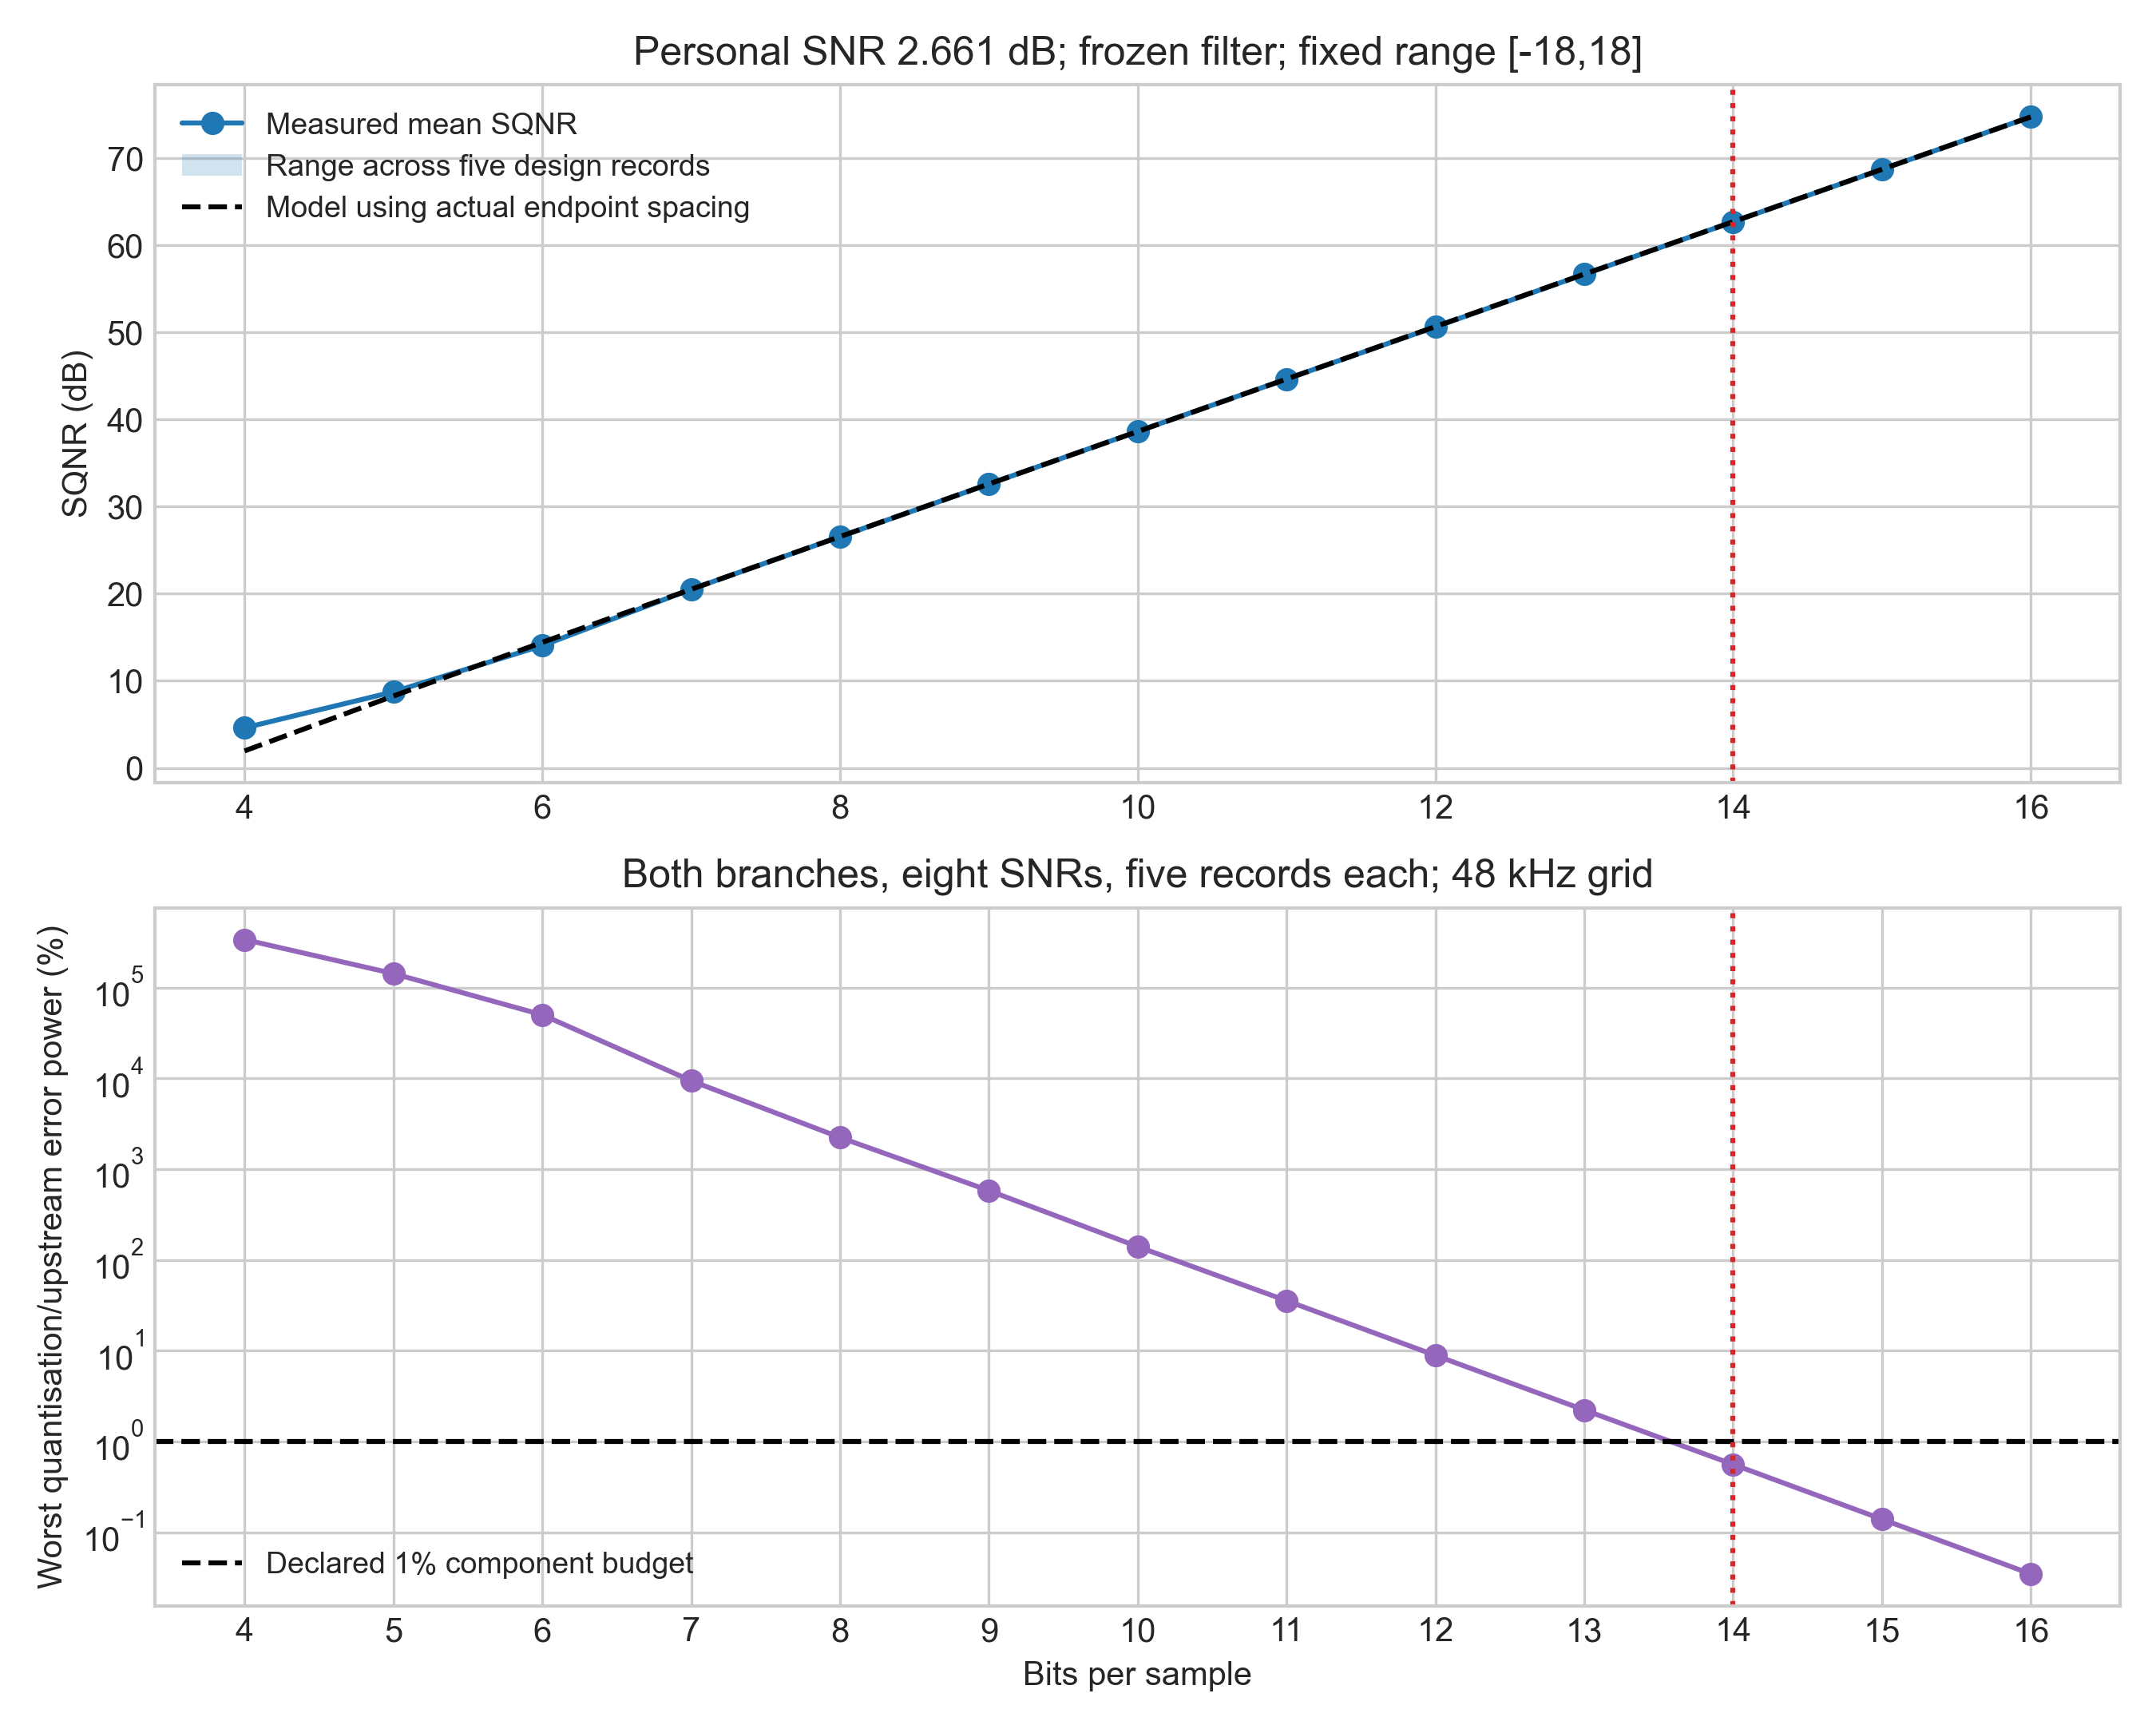
\includegraphics[width=.80\linewidth]{images/r31_sqnr_selection.png}
\caption{Measured SQNR and the declared component budget. Shading is the five-record design range, not a confidence interval; the low-bit model mismatch is retained.}
\label{fig:r31selection}
\end{figure}

At the anchor filtered point, measured SQNR is \QPersonalSqnr\,dB
(range [\QPersonalMin,\QPersonalMax]), model mean \QPersonalModel\,dB
and quantisation MSE $\QPersonalMse $. Complete-grid MSE changes from
$\QPersonalBefore $ to $\QPersonalAfter $. The 1 \% component budget permits
a 21 \% worst-case total-MSE change through cross terms
(Eq.~\eqref{eq:r31-total-bound}); the largest observed increase is
 \QMaxTotalPercent\%. A noisier input can have higher SQNR while being
less faithful to the reference, motivating the whole-chain metric in R4.

Fourteen bits uses 448000 information bits per record, 12.5 \% fewer than 16 bit.
Unsigned, sample-major, MSB-first packing is fixed; shared $ A,B $, length
and order are simulation metadata, not an assumed protected header.
All 131056 labels across the scanned widths round-trip, and independent
threshold quantisation/direct convolution/SciPy reconstruction reproduce
all 40 noise inputs and 1040 measurements. The quantiser freeze and
complete SQNR/error records remain under \path{stage3/r31/results/}.

\FloatBarrier
\subsection{Choose and explain the error-correcting code}
\label{sec:r32}
I select the taught systematic Hamming(7,4): length 7, four information
bits, rate $4/7 $, $ d_{\min}=3 $ and guaranteed correction $ t=1 $ \citep{hamming1950codes}.
With row messages, encoding is $\boldsymbol c=\boldsymbol mG\pmod2 $;
the receiver computes $\boldsymbol s=\boldsymbol rH^T\pmod2 $, matches
the actual $ H $ column, flips that position and extracts the four systematic
bits. The reference uses integer matrix multiplication followed by modulo two.
The exact $ G,H $, distance proof and worked examples are in
Appendix~\ref{app:ecc}. Its columns are 110, 101, 011, 111, 100, 010, 001;
a syndrome integer is not a direct bit index. This code is not SECDED:
multiple errors can be miscorrected, and a zero final syndrome does not
prove recovery of the transmitted message.

\paragraph{Alternatives, error profile and declared selection.}
The alternatives are the implemented Hamming(15,11), also $ d_{\min}=3,t=1 $;
majority-decoded repetition(5,1), $ d_{\min}=5,t=2 $; and uncoded(1,1).
The code constructions and exact decoder expectations are derived in
Appendix~\ref{app:ecc}. A higher Hamming rate does not increase correction
capability. Actual iid BSC flips produce binomial block multiplicities,
not an artificial one-flip restriction (Figure~\ref{fig:r32-profile}).
For the verified decoders, low-$ p $ BER begins at $9p^2 $ for (7,4),
versus $21p^2 $ for (15,11).

\begin{figure}[htbp]
 \centering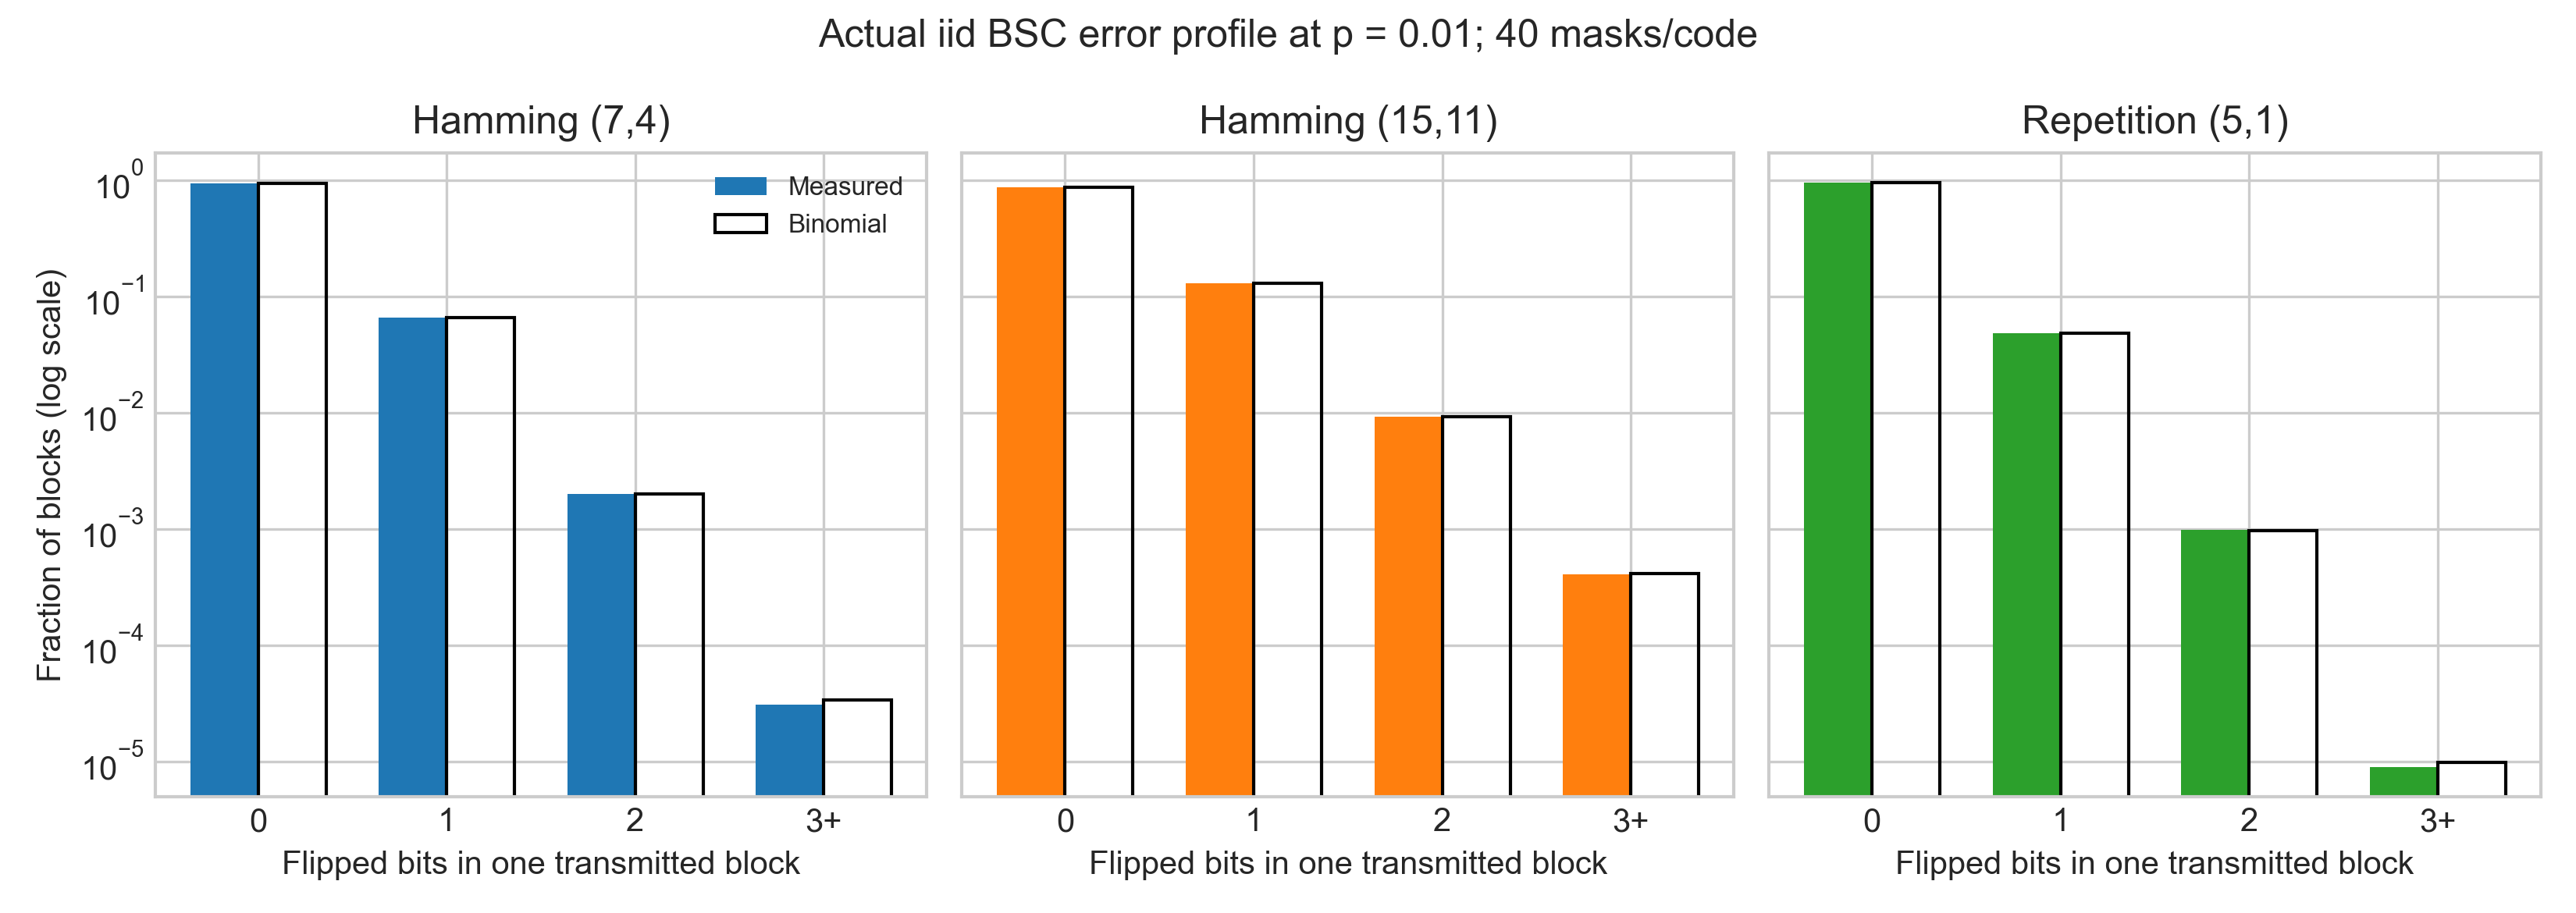
\includegraphics[width=.86\linewidth]{images/r32_block_profile.png}
 \caption{Actual BSC multiplicities versus the binomial model. Both Hamming codes correct one error; repetition corrects two at fivefold traffic cost.}
 \label{fig:r32-profile}
\end{figure}

The pilot reuses five R3.1 anchor-SNR inputs, with eight independent
masks per positive $ p $/code and one identity control per bank/code:
1140 cases, 1120 positive-$ p $ masks. The prespecified probabilities are
$0,10^{-4},0.001,0.003,0.01,0.03,0.1,0.3 $.
Five input banks are the independent units for selection; 40 masks are not
40 independent Gaussian inputs. Before BSC generation I fix expansion
$ M_t/M_b\le2 $ and equal selection weights over
$\mathcal P=\{0.001,0.003,0.01,0.03\}$:
\begin{equation}
 J_{c,g}=\frac14\sum_{p\in\mathcal P}
  \frac{\overline D_{c,p,g}}{\overline D_{\mathrm{uncoded},p,g}},
 \qquad J_c=\frac15\sum_{g=0}^4J_{c,g}.
 \label{eq:r32-score}
\end{equation}
Here $\overline D_{c,p,g}$ averages the eight full-grid MSEs in one bank.
The normalisation prevents high-$ p $ absolute loss alone determining the
score. Choose the eligible ECC with smallest $ J_c<1 $.

\begin{table}[htbp]
 \centering\small
 \caption{Defined alternatives and phase-0 selection score. Feasibility uses the declared twofold expansion budget, not the later rate cap.}
 \label{tab:r32-selection}
 \begin{tabular}{lrrrrrrr}
\toprule
Code & $n$ & $k$ & $d_{\min}$ & $t$ & Expansion & kbit/s & $J$ \\
\midrule
Uncoded & 1 & 1 & 1 & 0 & 1.00000 & 224 & 1.00000 \\
Hamming (7,4) & 7 & 4 & 3 & 1 & 1.75000 & 392 & 0.08344 \\
Hamming (15,11) & 15 & 11 & 3 & 1 & 1.36366 & 305.46 & 0.19204 \\
Repetition (5,1) & 5 & 1 & 5 & 2 & 5.00000 & 1120 & 0.01920 \\
\bottomrule
\end{tabular}

 
 
\end{table}

Hamming(7,4) has $ J=\ECCScore $, approximate pointwise 95 \% interval
$[\ECCScoreLow,\ECCScoreHigh]$, against 0.19204 for (15,11).
The paired difference is $-0.10860 $, interval $[-0.11311,-0.10410]$.
Repetition improves further ($ J=0.01920 $) but needs fivefold expansion.
A 1.5/2/5-fold budget would instead select (15,11)/(7,4)/repetition;
the twofold budget is a project resource preference, not a physical limit.

\paragraph{Framing, waveform meaning and verification.}
Equation~\eqref{eq:r32-framing} counts real bits, padding and sent bits.
H74 uses 784000 bits, no padding, 392 kbit/s; H15 uses 610920 bits, eight
padding bits, 305.46 kbit/s. Repetition uses 2240000 bits, 1120 kbit/s.
These are logical traffic rates for two seconds of source, not throughput
or equal-energy measurements. Padding is removed only after decoding;
real-payload BER and padded-block failure have different denominators.
Natural-binary bit significance and joint decoded errors mean BER alone
cannot rank NMSE (Eq.~\eqref{eq:r32-labelerror}).
An independent correction-sphere lookup decoder checks all 32930 received
words across the four layouts and replays all 1140 pilot cases. It agrees
on payload hashes, errors and full-grid MSE; $ p=0 $ recovers the exact
prechannel labels. The receiver gets only received bits and public metadata.
This frozen, phase-0 choice is subsequently tested on new records in R3.4.

\FloatBarrier
\subsection{Choose the error range before the personal draw}
\label{sec:r33}
The positive main range spans three decades:
\begin{equation}
 \mathcal P_{\rm main}=
 \{10^{-4},\,3\times10^{-4},\,10^{-3},\,3\times10^{-3},
       \,10^{-2},\,3\times10^{-2},\,10^{-1}\}.
 \label{eq:r33-grid}
\end{equation}
I add an identity control $ p=0 $, the anchor-seed point, and stress
points $0.2,0.3,0.5 $, giving 12 distinct conditions.
Table~\ref{tab:r33-range} links this range to the taught BSC and actual
code, rather than assuming a physical link's error distribution.

\begin{table}[htbp]
 \centering\small
 \caption{Frozen range and stress conditions. Each positive condition exposes 4480000 Hamming blocks; the identity control has 560000. Capacity and finite-code failure are different quantities.}
 \label{tab:r33-range}
 \begin{tabular}{rlrrr}
\toprule
$p$ & Role & $C(p)$ & $\Pr(J>1)$ & Expected failed blocks \\
\midrule
0 & Identity & 1.00000 & $0$ & 0.000 \\
0.0001 & Main grid & 0.99853 & $2.0993\times10^{-7}$ & 0.940 \\
$p_{\rm ID}$ & Anchor & 0.99712 & $9.3425\times10^{-7}$ & 4.185 \\
0.0003 & Main grid & 0.99606 & $1.8881\times10^{-6}$ & 8.459 \\
0.001 & Main grid & 0.98859 & $2.0930\times10^{-5}$ & 93.767 \\
0.003 & Main grid & 0.97054 & $1.8712\times10^{-4}$ & 838.291 \\
0.01 & Main grid & 0.91921 & $2.0310\times10^{-3}$ & 9099.067 \\
0.03 & Main grid & 0.80561 & $1.7093\times10^{-2}$ & 76576.793 \\
0.1 & Main grid & 0.53100 & $1.4969\times10^{-1}$ & 670630.912 \\
0.2 & Stress & 0.27807 & $4.2328\times10^{-1}$ & 1896308.736 \\
0.3 & Stress & 0.11871 & $6.7058\times10^{-1}$ & 3004210.944 \\
0.5 & Stress & 0.00000 & $9.3750\times10^{-1}$ & 4200000.000 \\
\bottomrule
\end{tabular}

 
 
\end{table}

At $10^{-4}$ the exposure predicts 1792 uncoded and 3136 coded raw flips,
but only 0.94049 failed Hamming blocks; observing none has probability
about 0.3904. Three failures occurred, versus 94 at $10^{-3}$
(expectation 93.76687). Exact pointwise binomial intervals and theoretical
BER accompany these rare counts; zero counts would not prove zero risk
(Appendix~\ref{app:statistics}). Even 4480000 blocks do not provide
a precise low-end decoded-BER estimate.

At $ p=0.1 $, the actual decoder's block failure probability is 0.1496944:
multiple errors are substantial. The rate--capacity crossing is
$ p=\PCapacityRoot $, while decoded BER loses its advantage at
$ p=\PBerRoot $ (Appendix~\ref{app:ecc}). They are different boundaries;
capacity does not guarantee short-code performance or waveform success \citep{shannon1948communication}.
Points 0.2/0.3 straddle the latter. At 0.5, capacity is zero, received bits
are independent of the payload and decoded BER is 0.5, providing a severe
sanity check. Stress points do not enter the personal mapping.

\paragraph{Reproducible anchor-seed convention.}
After freezing the range and observation budget, parameter leaf $(0,1)$
uses NumPy 2.1.3 SeedSequence(pool size 4)/PCG64 with root 2470964:
\begin{equation}
 U_p\sim U[0,1),\qquad
 \log_{10}p_{\rm ID}=-4+3U_p,\qquad
 p_{\rm ID}=10^{-4+3U_p}.
 \label{eq:r33-mapping}
\end{equation}
\begin{equation}
 U_p=\PUniform,\qquad p_{\rm ID}=\PPersonal.
 \label{eq:r33-personal}
\end{equation}
Equal logarithmic intervals have equal weight; the induced density is
derived in Appendix~\ref{app:random}. This is a declared project mapping,
not an externally specified algorithm or a physical distribution of channels.
Each experiment holds $ p $ fixed. Code and grid were not changed after
seeing the draw. The study marks 570 reused and 320 additional cases
explicitly, so its 890 cases/880 positive masks do not double-count
observations. Independent replay verifies every payload and error profile;
range, parameter state and protocol are frozen before R3.4 validation.

\FloatBarrier
\subsection{Measured coding gain under one success rule}
\label{sec:r34}
Success is acceptable \emph{population mean full-record NMSE}, distinct
from individual-waveform or bit-perfect success. Before validation,
the phase-0 no-bit-error baseline $ d_0=\CDesignBase $ fixes
\begin{equation}
 \tau=2d_0=\CTau,\qquad
 D_{\max}=P_x\tau=\CTauMse.
 \label{eq:r34-budget}
\end{equation}
The factor two is a project preference, not a universal or perceptual limit.
Both paths retain the same threshold; the new $ p=0 $ mean $\CNewBase $
does not recalibrate it. Total error retains upstream/channel cross terms
(Eq.~\eqref{eq:r34-cross}).
The 12 R3.3 conditions plus prespecified refinements $0.002,0.004,0.005 $
are tested with 300 new Gaussian inputs, 8400 positive-$ p $ masks and 9000
path records. Whole records are the independent units; Gaussian inputs
are shared across probabilities and layouts, so curves are dependent.
\begin{equation}
 \text{Gaussian: }(1,3,1,5,r),\qquad
 \text{BSC: }(2,3,1,c,r,\ell),\quad r=0,\ldots,299,\quad\ell=0,1.
 \label{eq:r34-paths}
\end{equation}
The earlier nested-bank variance estimate plans 300 records with half-width
target $0.1\tau $ near the two design boundaries; no validation result
changes the count. Approximate Bonferroni t/CLT intervals cover the finite
30-mean family (Appendix~\ref{app:statistics}), not a continuous-$ p $ band
or individual future records. The common rule and requested gain set are
\begin{equation}
 \operatorname{status}=
 \begin{cases}
 \mathrm{pass},&U\le\tau,\\
 \mathrm{fail},&L>\tau,\\
 \mathrm{inconclusive},&\text{otherwise}.
 \end{cases}
 \label{eq:r34-decision}
\end{equation}
\begin{equation}
 \mathcal G_{\rm tested}=
 \{p:\ U_{\rm coded}(p)\le\tau
          \ \text{and}\ L_{\rm uncoded}(p)>\tau\}.
 \label{eq:r34-gain}
\end{equation}

\begin{table}[htbp]
 \centering\small
 \caption{Independent NMSE means and approximate 30-family intervals, 300 records per path/condition. Gain means coded pass and uncoded fail at the same fixed threshold; decisions use unrounded CSV.}
 \label{tab:r34-quality}
 \begin{tabular}{rlll}
\toprule
$p$ & Uncoded mean [adjusted CI] & Hamming mean [adjusted CI] & Gain \\
\midrule
$0$ & 0.0291 [0.0289,0.0292] & 0.0291 [0.0289,0.0292] & no \\
$0.0001$ & 0.0873 [0.0825,0.0922] & 0.0292 [0.0289,0.0294] & yes \\
$p_{\rm ID}$ & 0.1516 [0.1449,0.1582] & 0.0292 [0.0290,0.0294] & yes \\
$0.0003$ & 0.2068 [0.1990,0.2146] & 0.0292 [0.0290,0.0295] & yes \\
$0.001$ & 0.6223 [0.6087,0.6360] & 0.0333 [0.0321,0.0346] & yes \\
$0.002$ & 1.2219 [1.2007,1.2431] & 0.0436 [0.0416,0.0457] & yes \\
$0.003$ & 1.7901 [1.7653,1.8149] & 0.0638 [0.0603,0.0673] & no \\
$0.004$ & 2.3823 [2.3534,2.4112] & 0.0922 [0.0877,0.0967] & no \\
$0.005$ & 2.9606 [2.9275,2.9936] & 0.1196 [0.1143,0.1249] & no \\
$0.01$ & 5.8943 [5.8475,5.9411] & 0.3970 [0.3866,0.4074] & no \\
$0.03$ & 17.2616 [17.1866,17.3365] & 3.1534 [3.1229,3.1839] & no \\
$0.1$ & 53.2739 [53.1572,53.3906] & 27.3053 [27.2175,27.3931] & no \\
$0.2$ & 94.8705 [94.7203,95.0206] & 75.2253 [75.0877,75.3630] & no \\
$0.3$ & 124.6956 [124.5513,124.8398] & 115.9078 [115.7615,116.0540] & no \\
$0.5$ & 148.9787 [148.8422,149.1151] & 149.0071 [148.8766,149.1377] & no \\
\bottomrule
\end{tabular}

 
 
\end{table}


\begin{figure}[htbp]
 \centering
 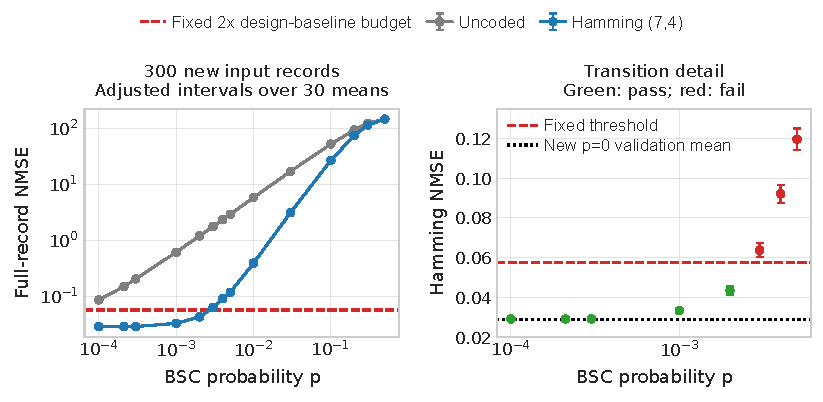
\includegraphics[width=.86\linewidth]{supporting/publication_r34_quality_gain_horizontal.pdf}
 \caption{Coded/uncoded mean quality over the full envelope (left) and the coded transition detail (right). Error bars use the frozen 30-mean family; the threshold is fixed before validation.}
 \label{fig:r34-quality}
\end{figure}

The primary measured gain is
\begin{equation}
 \boxed{\mathcal G_{\rm tested}
   =\{0.0001,\ p_{\rm ID},\ 0.0003,\ 0.001,\ 0.002\}}.
 \label{eq:r34-result}
\end{equation}
At the anchor point, coded/uncoded mean NMSE is
$\CPersonalCoded/\CPersonalUncoded $; the respective intervals lie below
and above $\tau $. The largest coded passing test point is 0.002; 0.003
fails. Uncoded $ p=0 $ passes, whereas $10^{-4}$ fails. These are tested
brackets, not exact continuous crossings. At higher $ p $ both fail quality
even where coding still reduces BER. The ancillary mean paired
reconstruction-error gain is \CPersonalGainDb\,dB, pointwise 95 \%
interval $[\CPersonalGainLow,\CPersonalGainHigh]$; it is not an $ E_b/N_0 $
gain or the log ratio of two mean MSEs.

\paragraph{Three meanings of success and the resource cost.}

\begin{figure}[htbp]
 \centering
 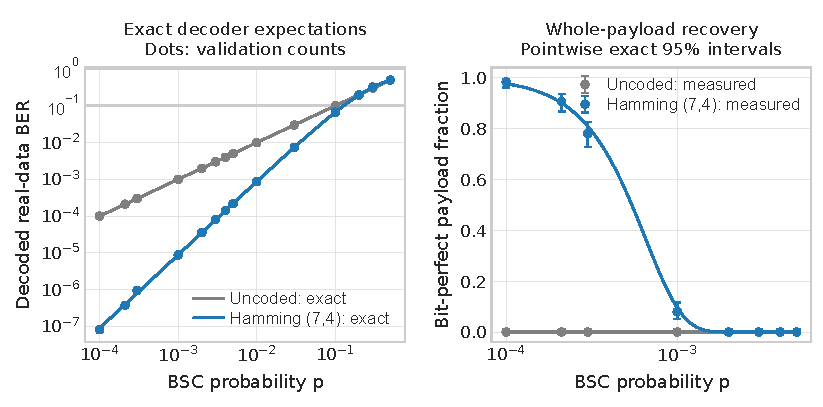
\includegraphics[width=.86\linewidth]{supporting/publication_r34_bit_recovery_horizontal.pdf}
 \caption{BER versus exact decoder expectations (left); complete 448000-bit payload recovery with pointwise 95\% proportion intervals (right). Zero BER counts are omitted from the log axis.}
 \label{fig:r34-bits}
\end{figure}

At $ p=0.002 $ the coded mean passes, 264/300 individual waveforms pass,
and 0/300 complete payloads are bit-perfect. At the anchor point all 300
coded waveforms pass but only \CPerfectPersonal/300 payloads are perfect;
both uncoded counts are zero. The coded perfect-payload estimate is
 \CPerfectPersonalPercent\%, pointwise exact 95 \% interval
$[\CPerfectPersonalLow,\CPerfectPersonalHigh]\%$; its theoretical value is
 \CPerfectPersonalTheory\% (Eq.~\eqref{eq:r34-payload}).
These digital-message probabilities differ from the 30-family waveform
mean intervals. The exact BER/block laws describe actual independent BSC
flips, not an imposed single-flip experiment.

Prespecified threshold factors 1.5, 2, 4 retain exclusive gain at $ p_{\rm ID}$,
0.0003 and 0.001. Other classifications can change: an interval crossing
the threshold remains inconclusive, not silently a pass.
The coded stream sends 784000 bits versus 448000 uncoded: 75 \% overhead,
392 versus 224 kbit/s, within the twofold budget. Equal $ p $ is not equal
traffic or energy. Alternative-method replay (Section~\ref{sec:r61})
verifies all 9000 paths/decisions within MSE $4.27\times10^{-14}$;
no overload was observed.
This establishes a conditional result for the supplied record, fixed
anchor SNR, framing and budget, rather than universal code optimality.

\FloatBarrier
\section{Stage 4: End-to-end measurement and evaluation}
\subsection{Why whole-record NMSE, with MAE as an alternative}
\label{sec:r41}
I retain $ D=\operatorname{mean}[(\widehat x-u)^2]$ and
$ d=D/P_u $, $ P_u=\MReferencePower $, over all 96000 original positions.
The definition measures full-record squared reconstruction error
relative to the original reference power.
Appendix~\ref{app:metrics} derives the common definitions, bias identity,
MAE/RMSE relation and dB conventions. NMSE is dimensionless, lower is
better and it can exceed one; amplitude gain, timing and endpoints are
not fitted or trimmed. Centred variance alone would hide fixed bias.

MAE is a genuinely different loss; RMSE is a monotone transformation of
per-record MSE. Figure~\ref{fig:r41-ranking} shows why the choice matters:
diffuse error has $(D,\mathrm{MAE})=(0.01,0.1)$, sparse large errors
$(0.04,0.02)$. MAE prefers the latter, NMSE the former.
Natural-binary MSB errors are $2^{13}$ times the amplitude of LSB errors
at 14 bit ($2^{26}$ in squared error), supporting a loss sensitive to
large corruption. These local ratios do not determine total NMSE.

\begin{figure}[htbp]
 \centering
 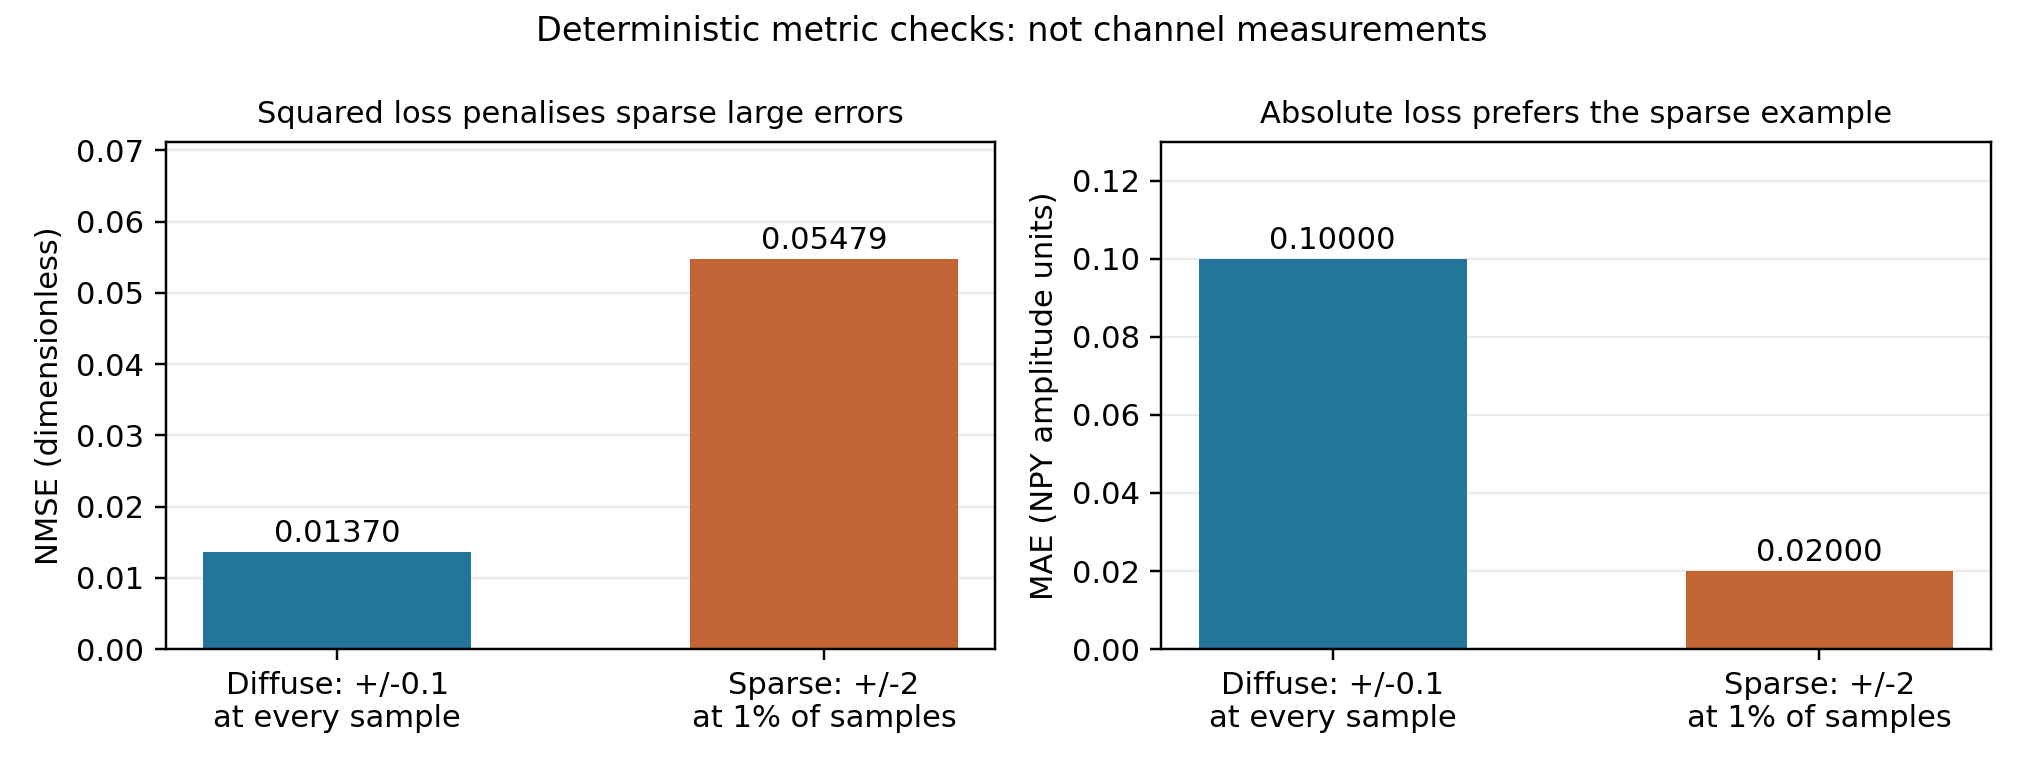
\includegraphics[width=.76\linewidth]{images/r41_metric_ranking.png}
 \caption{Declared full-grid metric counterexamples. NMSE favours diffuse small error, MAE the sparse large error. Axes retain their different units; this is not a stochastic channel experiment.}
 \label{fig:r41-ranking}
\end{figure}

MAE remains a diagnostic; neither metric is claimed as perceptual quality
\citep{wang2009mse}.
Correlation alone is insufficient: $\widehat x=2u $ has correlation one
but NMSE one. Likewise exact bit delivery retains upstream waveform
error. For repeated records I distinguish $-10\log_{10}\bar d $ from
the mean of individual dB ratios. Seven semantic checks/221 independent
assertions and the saved R3 examples verify these interpretations.

\FloatBarrier
\subsection{Four configurations and what their contrasts isolate}
\label{sec:r42}
Filter switch $ f $ and code switch $ c $ vary while sampling, Gaussian/BSC
models, quantiser, framing and receiver remain common. Here $ x $ contains
32000 transmission samples; $\mathcal R $ returns 96000 reference-grid
positions and $ d_{fc}$ denotes their full-record NMSE:
\begin{align}
 y&=x+\eta,\quad z_f=F_f(y),\quad
 b_f=\operatorname{pack}(\mathcal Q(z_f)),\nonumber\\
 t_{fc}&=E_c(b_f),\quad r_{fc}=t_{fc}\oplus\varepsilon_c,\nonumber\\
 \widehat x_{fc}&=\mathcal R\!\left[
 \mathcal Q^{-1}\!\left(\operatorname{unpack}(D_c(r_{fc}))\right)\right].
 \label{eq:r42-chain}
\end{align}
Here $ F_0=E_0=D_0=I $; $ F_1 $ is the frozen FIR and $ E_1,D_1 $ the taught
Hamming(7,4). Neither bypasses the protective modules, not the degradations.
Code-only quantises noisy unfiltered samples; filter-only sends unprotected
bits through the BSC. The receiver has only received bits and public
codebook/framing/output-length metadata, never the reference or true masks.

\begin{table}[htbp]
 \centering
 \small
 \caption{Four actual paths carrying 448000 real information bits. Gaussian noise, quantisation, BSC and reconstruction remain enabled in every configuration.}
 \label{tab:r42-configurations}
 \begin{tabular}{llrrr}
\toprule
ID & Configuration & $f$ & $c$ & Sent bits / logical kbit/s \\
\midrule
00 & neither & 0 & 0 & 448000 / 224 \\
10 & filter-only & 1 & 0 & 448000 / 224 \\
01 & code-only & 0 & 1 & 784000 / 392 \\
11 & both & 1 & 1 & 784000 / 392 \\
\bottomrule
\end{tabular}

 
 
\end{table}

One Gaussian vector is shared within each $(S,r)$ across all four paths
and $ p $ values. Same-code filter pairs replay the same BSC leaf and shape;
uncoded/coded layouts have independent masks and unequal lengths.
\begin{align}
 \text{Gaussian}:&(1,4,a,\mathrm{SNR\ ID},r),\nonumber\\
 \text{BSC}:&(2,4,a,\mathrm{joint\ ID},r,\mathrm{layout\ ID}).
 \label{eq:r42-rng}
\end{align}
At $ p=0 $ no mask is drawn. The actual decoder's translation identity
(Eq.~\eqref{eq:r42-pair-invariant}) gives equal XOR error patterns/BER
within 00/10 and 01/11, while their waveform NMSE can differ through
bit values, upstream errors and amplitude-error signs.
The conditional reductions and interaction are
\begin{align}
 g_{F\mid c=0}&=d_{00}-d_{10},&
 g_{F\mid c=1}&=d_{01}-d_{11},\nonumber\\
 g_{C\mid f=0}&=d_{00}-d_{01},&
 g_{C\mid f=1}&=d_{10}-d_{11},\nonumber\\
 I&=d_{00}-d_{10}-d_{01}+d_{11}.
 \label{eq:r42-effects}
\end{align}
Positive reductions improve quality; negative values are retained.
Comparisons at fixed $ c $ isolate enabling the filter; those at fixed $ f $
isolate enabling ECC including its extra transmitted bits. Comparing only
00 with 11 confounds these effects. Interaction is not a responsibility
percentage, and these switches do not separately identify changing the
sampling rate or bit depth. Rates remain 224/392 kbit/s, not equal energy.

Twenty new pilot bundles over 22 unique conditions produce 1760 paths.
All are independently replayed; mask invariants and clean/identity controls
pass. Pilot variance alone plans 1400 validation bundles for 88 condition
means plus four main-objective means, targeting 5 \% relative half-width.
The smallest passing multiple of 50 is frozen before phase 1
(Eq.~\eqref{eq:r42-planning}); a pilot prediction is not a guarantee of
achieved precision. No pilot observation enters the final means.

\FloatBarrier
\subsection{Central degradation curves and conditional contributions}
\label{sec:r43}
Figure~\ref{fig:r43-central} is the central end-to-end result: all four
actual configurations on two severity slices, holding $ p=p_{\rm ID}$ while
varying SNR and $ S=S_{\rm ID}$ while varying $ p $.
Eight SNR and 15 BSC conditions share one anchor point, hence 22 unique
conditions; this is not a full two-dimensional response surface.
The 1400 held-out bundles use disjoint phase-1 leaves:
\begin{equation}
 \text{Gaussian}: (1,4,1,s_G,r),\qquad
 \text{BSC}: (2,4,1,s,r,c),\quad r=0,\ldots,1399.
 \label{eq:r43-paths}
\end{equation}
There are \WPaths{} paths,\WGaussian{} unique Gaussian vectors and
 \WMasks{} positive-$ p $ masks. Reused inputs do not multiply independent
exposure. At $ p=0 $ Gaussian noise remains; 00=01 and 10=11 exactly.
Four no-Gaussian/$ p=0 $ controls run once outside the random means.

Approximate Bonferroni t/CLT intervals use 1400 complete bundles and the
prespecified 92-statistic family (Eq.~\eqref{eq:r43-mean-ci}); they are
mean intervals, not per-record spread or exact finite-sample guarantees.
The 12-condition main objective first averages each bundle's 12 equally
weighted, unique main conditions, then estimates uncertainty from 1400
bundle scores (Eq.~\eqref{eq:r43-main-objective}). Diagnostic/refinement
points have zero main weight; the personal overlap is counted once.
The weights are a design objective, not observed channel probabilities.

\begin{figure}[!htbp]
 \centering
 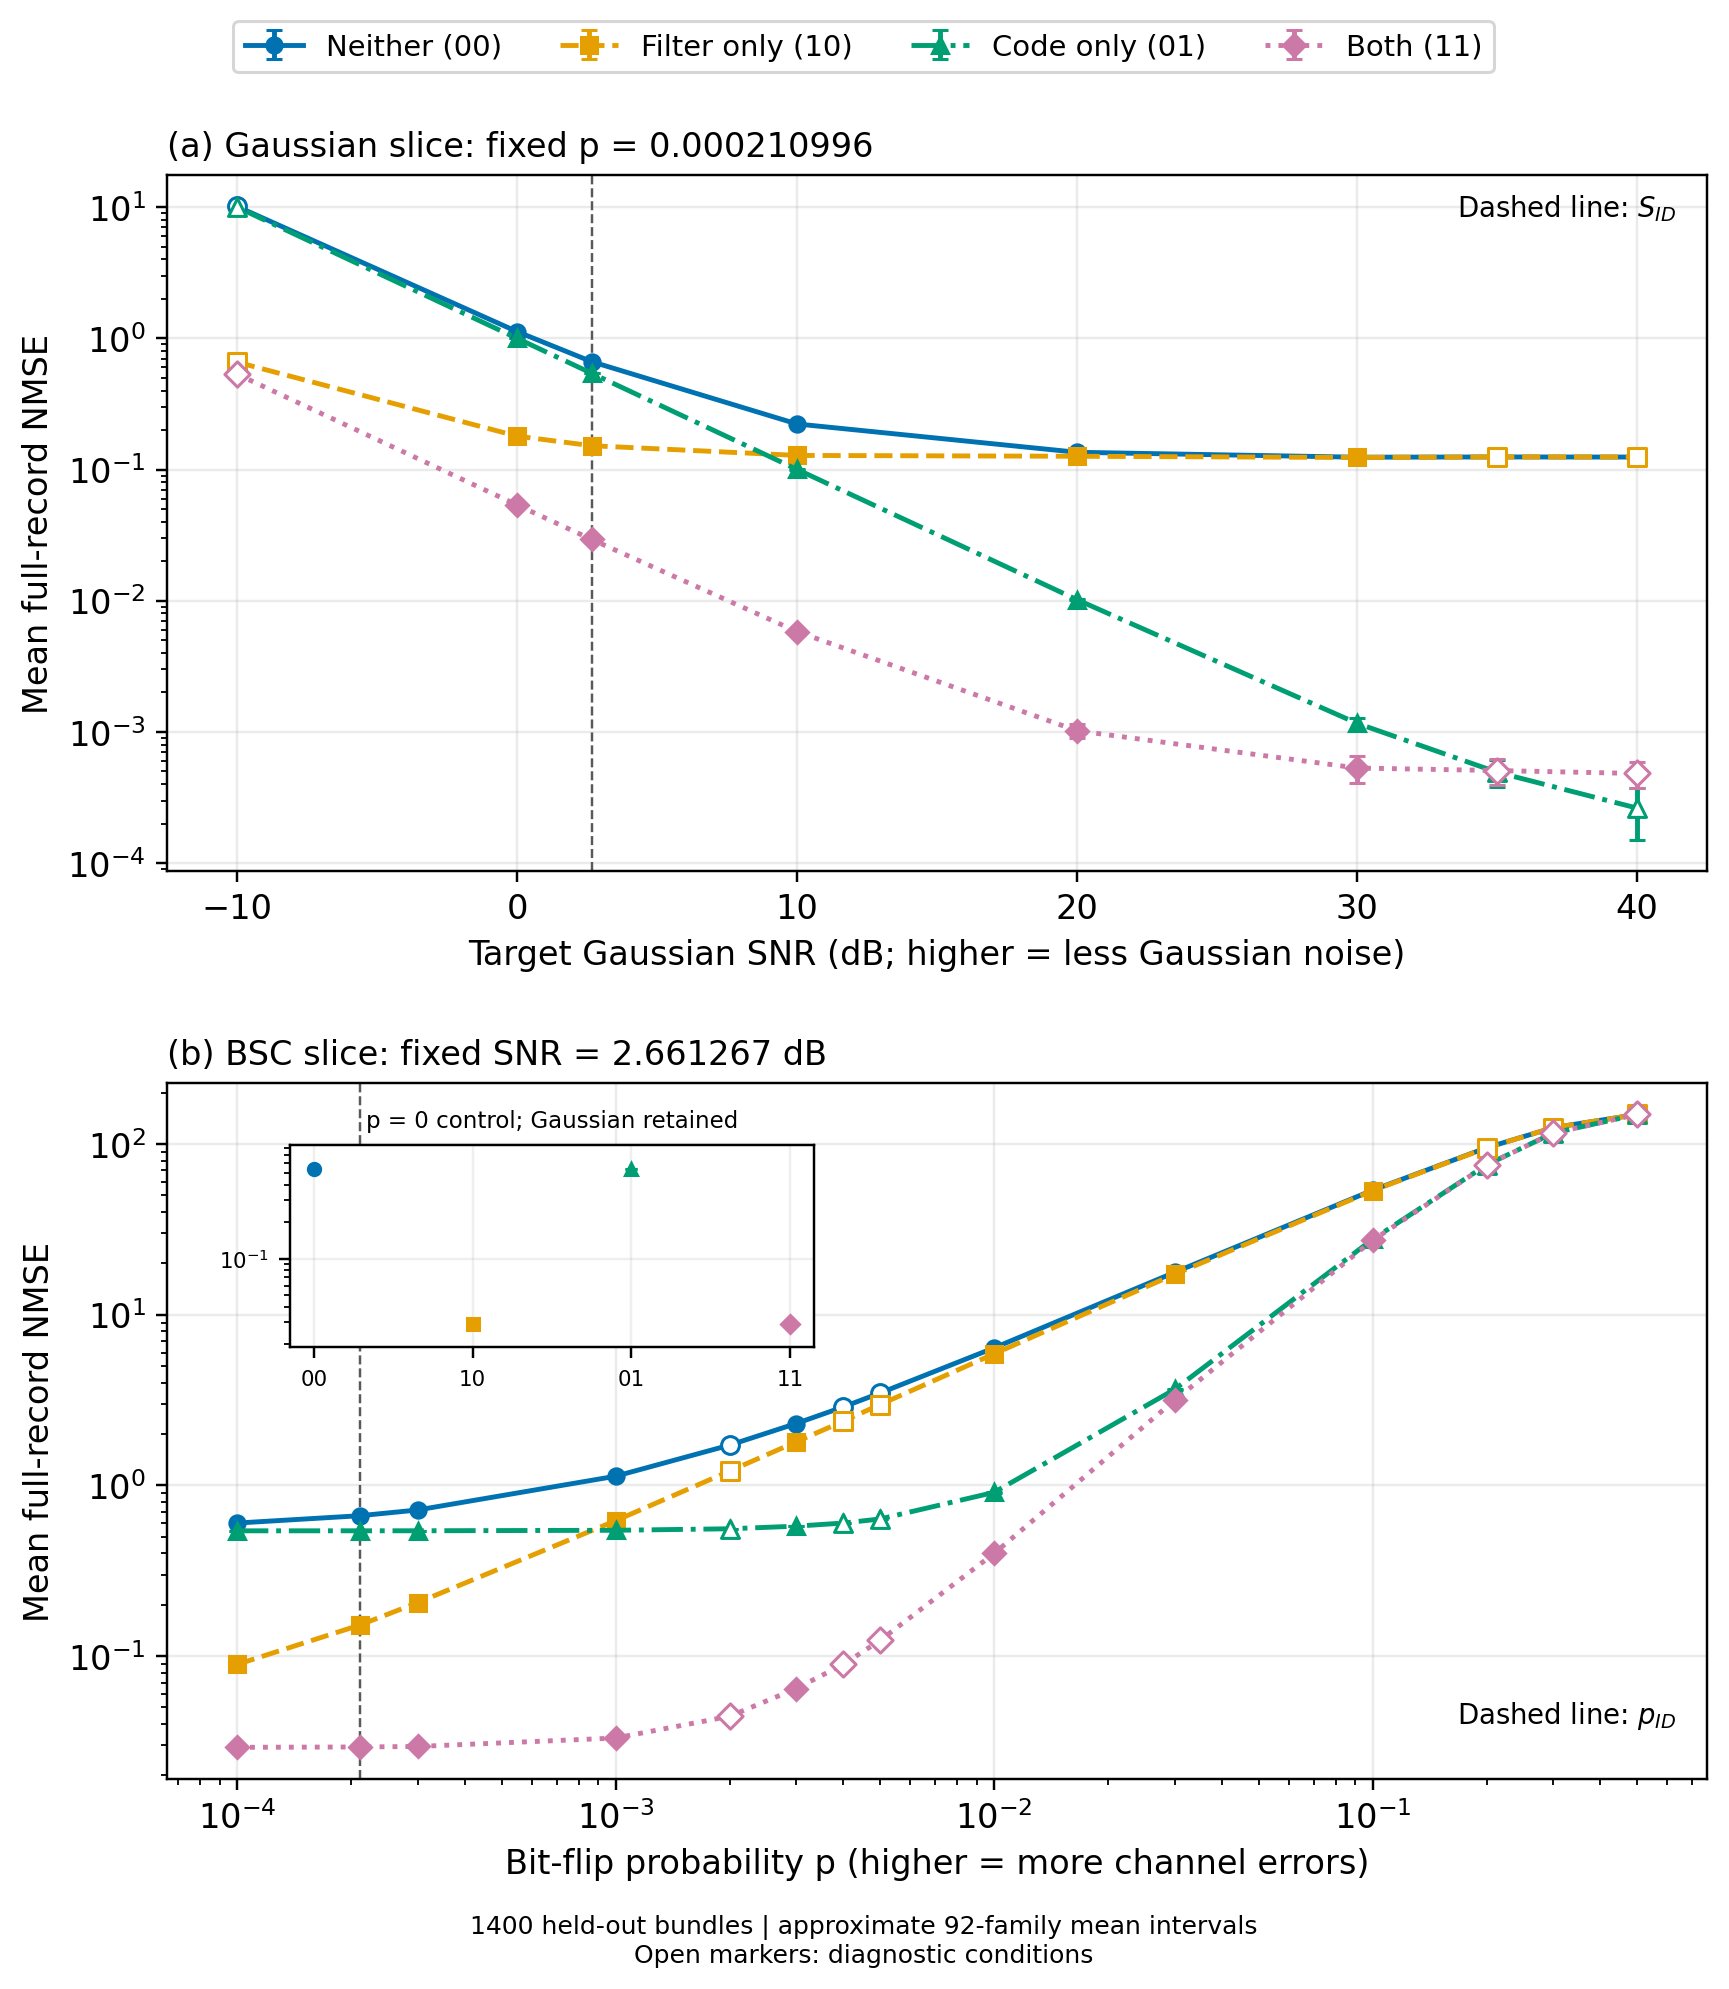
\includegraphics[width=.88\linewidth]{images/r43_central_quality.png}
 \caption{Four configurations, 1400 bundles, approximate 92-family mean intervals. Positive $p$: log axis; inset: $p=0$ with Gaussian retained. Filled/open: main/diagnostic points; lines join tested points only.}
 \label{fig:r43-central}
\end{figure}


\begin{table}[htbp]
 \centering\small
 \caption{Held-out anchor-point results. Only NMSE intervals belong to the 92-mean family; MAE and real-information BER are descriptive.}
 \label{tab:r43-personal}
 \begin{tabular}{lrrrr}
\toprule
Config. & Mean NMSE & Adjusted mean interval & Mean MAE & Data BER \\
\midrule
00 & 0.664309 & [0.660879, 0.667739] & 0.513143 & $2.1117\times10^{-4}$ \\
10 & 0.151933 & [0.148476, 0.155391] & 0.131631 & $2.1117\times10^{-4}$ \\
01 & 0.541989 & [0.541564, 0.542413] & 0.501820 & $3.7946\times10^{-7}$ \\
11 & 0.029339 & [0.029190, 0.029488] & 0.116303 & $3.7946\times10^{-7}$ \\
\bottomrule
\end{tabular}

 
 
\end{table}

% Keep the run-in heading and its complete result paragraph on the same page.
\noindent\begin{minipage}{\linewidth}
\paragraph{What the curves establish.}
At the anchor point, neither/filter-only/code-only/both mean NMSEs are
$\WPersonalNeither $, $\WPersonalFilter $, $\WPersonalCode $ and
$\WPersonalBoth $. Both gives the lowest error: coding alone leaves most
Gaussian error; filtering alone leaves unprotected bit corruption.
As SNR rises, the uncoded BSC floor persists. At 40 dB code-only/both means
are $\WHighCode/\WHighBoth $; the estimated filter reduction
$\WHighFilterReduction $ has conservative interval
$[\WHighFilterLower,\WHighFilterUpper]$, including zero.
The apparent reversal is therefore not established by the primary rule.
Separate clean controls do establish FIR distortion: NMSE
$\WCleanRaw $ without filtering and $\WCleanFilter $ with it.
\end{minipage}\par

\begin{table}[htbp]
 \centering\small
 \caption{Conditional NMSE reductions and interaction at the anchor/high-SNR points. Positive reductions improve quality; conservative intervals retain negative and unresolved effects.}
 \label{tab:r43-effects}
 \begin{tabular}{llrr}
\toprule
Condition & Contrast & Mean reduction & Conservative interval \\
\midrule
Personal & $G_{F\mid C=0}$ & $5.1238\times10^{-1}$ & $[5.0549\times10^{-1}, 5.1926\times10^{-1}]$ \\
Personal & $G_{F\mid C=1}$ & $5.1265\times10^{-1}$ & $[5.1208\times10^{-1}, 5.1322\times10^{-1}]$ \\
Personal & $G_{C\mid F=0}$ & $1.2232\times10^{-1}$ & $[1.1847\times10^{-1}, 1.2618\times10^{-1}]$ \\
Personal & $G_{C\mid F=1}$ & $1.2259\times10^{-1}$ & $[1.1899\times10^{-1}, 1.2620\times10^{-1}]$ \\
Personal & $I$ & $-2.7385\times10^{-4}$ & $[-7.7348\times10^{-3}, 7.1871\times10^{-3}]$ \\
40 dB & $G_{F\mid C=0}$ & $-2.1906\times10^{-4}$ & $[-7.1277\times10^{-3}, 6.6896\times10^{-3}]$ \\
40 dB & $G_{F\mid C=1}$ & $-2.1972\times10^{-4}$ & $[-4.4259\times10^{-4}, 3.1494\times10^{-6}]$ \\
40 dB & $G_{C\mid F=0}$ & $1.2422\times10^{-1}$ & $[1.2065\times10^{-1}, 1.2778\times10^{-1}]$ \\
40 dB & $G_{C\mid F=1}$ & $1.2422\times10^{-1}$ & $[1.2065\times10^{-1}, 1.2778\times10^{-1}]$ \\
40 dB & $I$ & $6.6129\times10^{-7}$ & $[-7.1309\times10^{-3}, 7.1322\times10^{-3}]$ \\
\bottomrule
\end{tabular}

 
 
\end{table}

The conditional contrasts above inherit conservative bounds from the
joint mean event (Appendix~\ref{app:statistics}); paired pointwise
intervals are separate exploratory results. Nonadditivity is retained.
At $ p=0.5 $ independently fair recovered labels predict NMSE 148.960954
for every configuration, and all four measured intervals contain it.
This is the random-label model of Appendix~\ref{app:quant}, not small
quantisation noise $\Delta^2/12 $.

\begin{table}[htbp]
 \centering\small
 \caption{Twelve-condition equal-weight objective from 1400 independent bundle scores. Intervals belong to the 92-statistic family; weights are design choices, not channel frequencies.}
 \label{tab:r43-objective}
 \begin{tabular}{lrrrr}
\toprule
Config. & $\bar J$ & Adjusted mean interval & Half-width (\%) & kbit/s \\
\midrule
00 & 7.06272 & [7.05624, 7.06919] & 0.09 & 224 \\
10 & 6.65633 & [6.64974, 6.66293] & 0.10 & 224 \\
01 & 3.00505 & [3.00105, 3.00905] & 0.13 & 392 \\
11 & 2.58806 & [2.58400, 2.59211] & 0.16 & 392 \\
\bottomrule
\end{tabular}

 
 
\end{table}

The objective summarises only its declared 12-condition domain.
Using Eq.~\eqref{eq:r43-contrast}, adjacent objective differences
$J_{00}-J_{10}$, $J_{10}-J_{01}$ and $J_{01}-J_{11}$ have conservative
outward-rounded intervals $[0.39331,0.41946]$, $[3.64069,3.66188]$ and
$[0.40893,0.42506]$, respectively. All are positive on the approximate
joint mean event, supporting $J_{11}<J_{01}<J_{10}<J_{00}$ for these
weights. This weighted-average ranking does not assert the same ordering
at every SNR/$p$, or in a different channel population.

\begin{table}[htbp]
 \centering\small
 \caption{Configuration 11 full-grid component powers, including small terms, plus signed cross terms. Sampling-scale residuals here are numerical, not measurable aliasing.}
 \label{tab:r43-components}
 \begin{tabular}{lrr}
\toprule
Term (configuration 11) & Personal point & 40 dB, personal $p$ \\
\midrule
Sampling & $1.7504\times10^{-25}$ & $1.7504\times10^{-25}$ \\
Filter & $2.2951\times10^{-4}$ & $2.2951\times10^{-4}$ \\
Gaussian & $2.1061\times10^{-2}$ & $3.8852\times10^{-6}$ \\
Quantisation & $4.0242\times10^{-7}$ & $4.0240\times10^{-7}$ \\
Channel & $1.2600\times10^{-4}$ & $1.1830\times10^{-4}$ \\
Signed sum of 10 cross terms & $2.2131\times10^{-7}$ & $-2.0212\times10^{-8}$ \\
Total MSE & $2.1418\times10^{-2}$ & $3.5208\times10^{-4}$ \\
\bottomrule
\end{tabular}

 
 
\end{table}

% A top-of-page component table must not split this explanatory paragraph.
\noindent\begin{minipage}{\linewidth}
The five full-grid powers and ten signed cross terms sum to total MSE
(Eqs.~\eqref{eq:r42-components}, \eqref{eq:r42-component-power}).
Sampling residual, finite-FIR distortion, Gaussian error, quantisation
and channel-induced waveform change remain distinct; they are not forced
into a 100 \% responsibility chart. Earlier R1/R3 comparisons support the
fixed sampling/bit-width decisions; the four switches alone do not
identify their separate causal effects. MAE is retained in the personal
table to reveal sensitivity to large corruption.
\end{minipage}\par

\paragraph{Precision and numerical limits.}
Seven of 92 means miss the pilot's 5\% relative-half-width target,
reaching \WMaxRelativePercent\%. They are coded cases at 20--40 dB and
personal $p$: rare uncorrectable blocks had variance underestimated by the
20-bundle pilot. The frozen 1400 count is retained without optional stopping.
These percentages describe uncertainty in mean NMSE, not reconstruction
error; 5\% is a planning tolerance. At 40 dB the coded filter contrast
crosses zero (Table~\ref{tab:r43-effects}), leaving its sign unresolved.
Personal comparisons and the four objective means have separate reported
intervals; all objective means meet the target, but the positive contrast
bounds, not target compliance, support their scoped ranking.
Computational agreement does not remove finite-sample uncertainty.

\begin{table}[htbp]
 \centering\small
 \caption{Four largest achieved relative half-widths. Joint IDs 19/20/21 are 30/35/40 dB at personal $ p $; the 5 \% planning target is not an achieved guarantee.}
 \label{tab:r43-precision}
 \begin{tabular}{lrr}
\toprule
Statistic (joint ID, config.) & Half-width (\%) & Target (\%) \\
\midrule
21, 01 & 42.43 & 5.00 \\
19, 11 & 23.56 & 5.00 \\
20, 01 & 23.36 & 5.00 \\
21, 11 & 23.11 & 5.00 \\
\bottomrule
\end{tabular}

 
 
\end{table}

Alternative-method replay (Section~\ref{sec:r61}) checks every
\WPaths{} path, all 92 means, hashes and component identities within MSE
$\WIndependentMse$. Full measurements, paired effects, seed/source records
and local examples are in \path{stage4/r43/results/}; excerpts do not
replace complete-record metrics.

\FloatBarrier
\Needspace{11\baselineskip}
\FloatBarrier
\section{Stage 5: Critical reflection}
\subsection{Identify the limiting tested decision}
\label{sec:r51}
For the declared 12-condition objective and original feasibility rules,
the limiting tested decision is retaining 14 bit in the existing
sequential natural-binary/Hamming layout. Increasing to 16 bit is the
only tested feasible change with a positive adjusted objective-gain
interval. Small quantisation power does not imply that this is simply
dominant quantisation noise; the experiment tests the complete chain.

R4's unchanged cohort diagnoses main-domain channel power
$\RfiveMainChannel $, Gaussian power $\RfiveMainGaussian $ and quantisation
power $\RfiveMainQuant $, retaining signed cross terms. This locates loss
but does not establish a causal design ranking. I therefore predeclare
nine one-decision variants: baseline; 385-tap half-width 60/80 Hz;
257/513 taps at 70 Hz; 16 bit; Hamming(15,11); repetition(5,1); no ECC.
Everything else retains the standard formulas, fixed matrices, original
signal, range and full-grid metric.

Twenty new study-5 pilot bundles plan 350 new confirmation bundles;
300 fails the frozen rule, 350 passes. Each bundle runs all nine variants
at 15 conditions: the 12 main conditions plus three zero-main-weight
diagnostics ($p=0.3,0.5$ at the anchor SNR, and 40 dB at the personal $p$).
Thus $350\times9\times15=47\,250$ confirmation paths are run;
only the 12 main conditions enter the objective. Eq.~\eqref{eq:r51-planning}
uses tolerance $\max(0.01,0.05|\bar g_{\rm pilot}|)$; actual confirmation
half-widths meet all frozen targets. The approximate 19-statistic family
contains eight main gains, eight personal gains and three personal
means for R5.2. Gains use Eq.~\eqref{eq:r51-gain}; whole bundles are
the independent units. R4 and pilot records do not enter these means.
Same layouts share masks within a bundle; changed lengths use separate
registered layouts. Alternative-method replay (Section~\ref{sec:r61})
checks all confirmation paths within MSE
$\RfiveIndependentMse$; kernels also pass cosine-sum checks.

\begin{table}[htbp]
 \centering\small
 \caption{New R5 confirmation: objective and paired gains from 350 bundles, approximate 19-family intervals. Feasibility means original 1 \% gain/twofold expansion rules; absolute rates remain visible.}
 \label{tab:r51-decisions}
 \begin{tabular}{llrrr}
\toprule
One change & Feasible & kbit/s & Mean $J$ & Paired $J$ reduction [interval] \\
\midrule
Half-width 60 Hz & No & 392.00 & 2.58890 & $1.4624\times10^{-3}\ [1.3297\times10^{-3},1.5952\times10^{-3}]$ \\
Half-width 80 Hz & No & 392.00 & 2.59431 & $-3.9526\times10^{-3}\ [-4.0412\times10^{-3},-3.8640\times10^{-3}]$ \\
257 taps & No & 392.00 & 2.61074 & $-2.0373\times10^{-2}\ [-2.0651\times10^{-2},-2.0096\times10^{-2}]$ \\
513 taps & Yes & 392.00 & 2.59185 & $-1.4839\times10^{-3}\ [-1.5551\times10^{-3},-1.4127\times10^{-3}]$ \\
16 bit & Yes & 448.00 & 2.42149 & $1.6887\times10^{-1}\ [1.5944\times10^{-1},1.7830\times10^{-1}]$ \\
Hamming(15,11) & Yes & 305.46 & 5.01125 & $-2.4209\times10^{0}\ [-2.4324\times10^{0},-2.4094\times10^{0}]$ \\
Repetition(5,1) & No & 1120.00 & 0.45581 & $2.1345\times10^{0}\ [2.1268\times10^{0},2.1423\times10^{0}]$ \\
Uncoded & Yes & 224.00 & 6.65212 & $-4.0618\times10^{0}\ [-4.0747\times10^{0},-4.0488\times10^{0}]$ \\
\bottomrule
\end{tabular}

 
 
\end{table}


\begin{figure}[htbp]
 \centering
 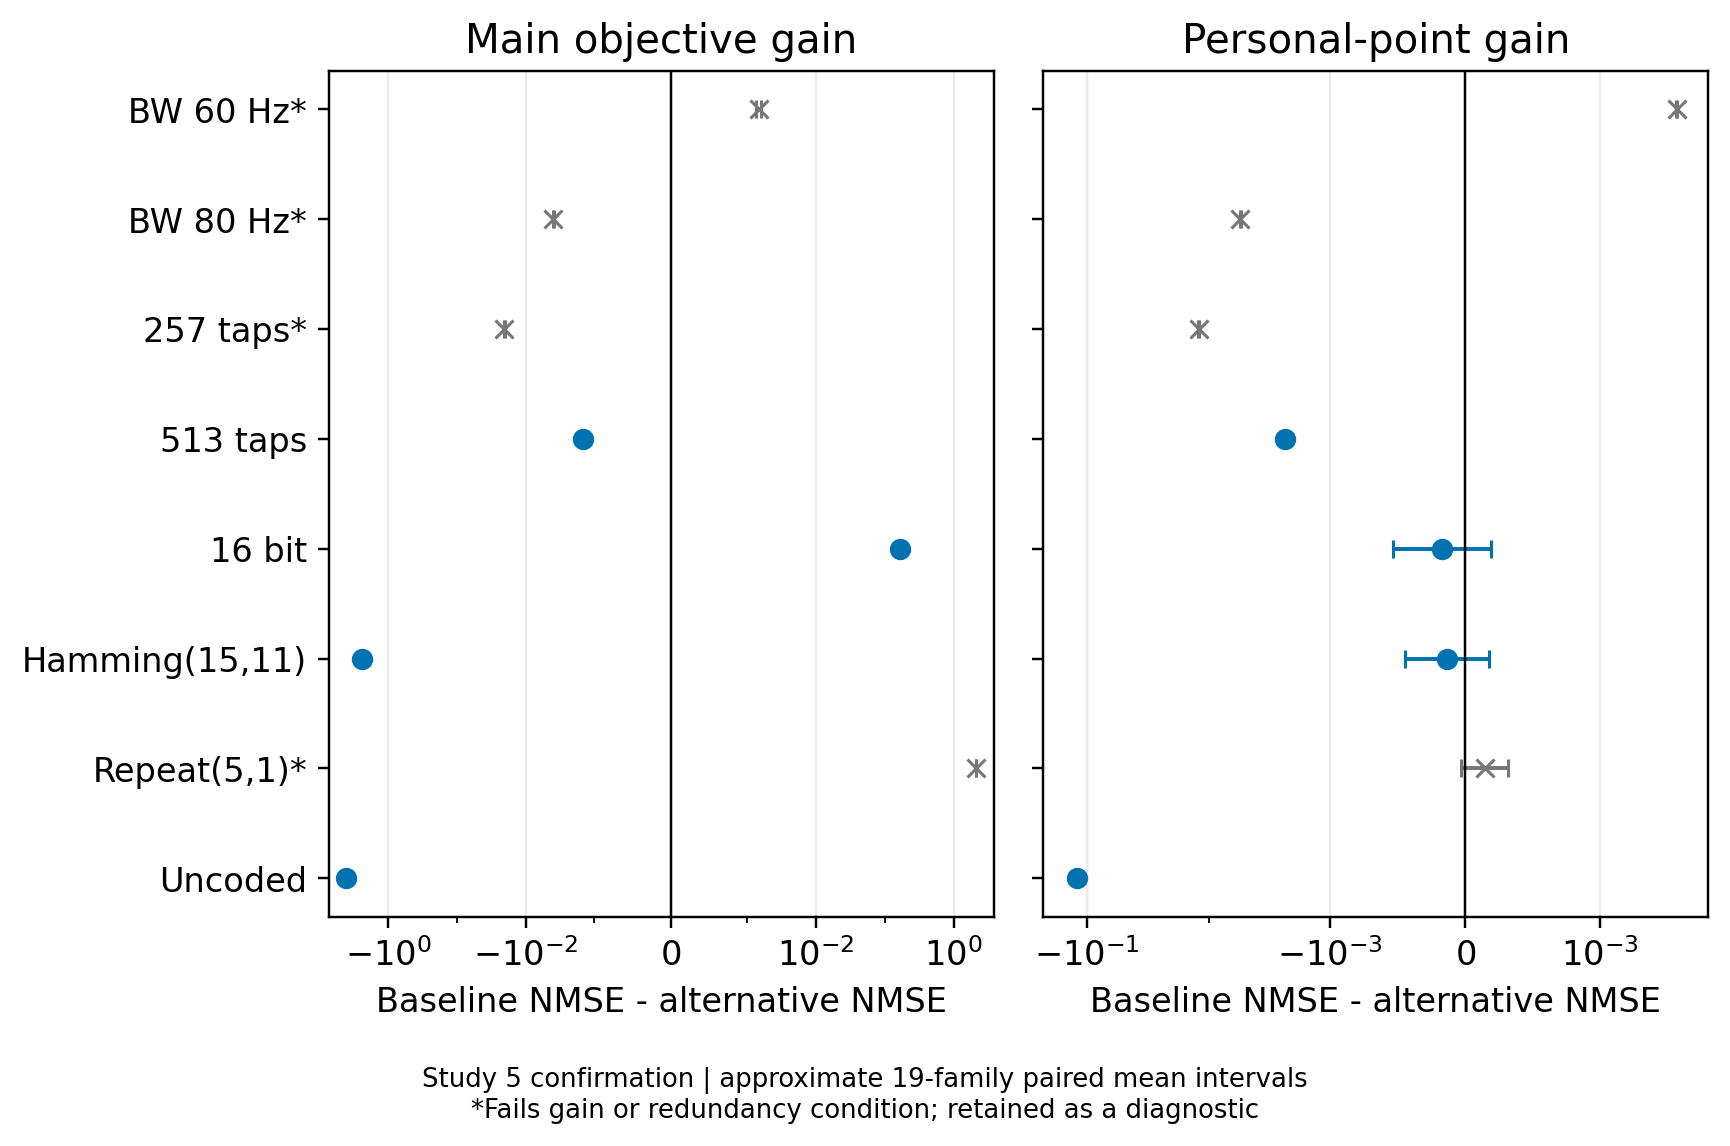
\includegraphics[width=.80\linewidth]{images/r51_counterfactual_gains.png}
 \caption{Single-decision gains with 19-family intervals. Grey crosses fail original feasibility rules; repetition cannot be a feasible winner. Symmetric-log panels retain negative/small effects and use distinct ranges.}
 \label{fig:r51-gains}
\end{figure}

\begin{samepage}
Baseline objective $\RfiveBaseJ $ falls with 16 bit by $\RfiveBitsGain $,
interval $[\RfiveBitsLower,\RfiveBitsUpper]$, at 392 $\to $448 kbit/s
(14.29 \% more traffic). Same-cohort prechannel improvement is only
$\RfiveBitsPreGain $. Most gain is in channel terms, not a 16-fold
total-error reduction predicted from $\Delta^2/12 $.
Eq.~\eqref{eq:r51-quant-ratio} gives the component ratio;
Eq.~\eqref{eq:r51-bit-coupling} retains joint decoded-bit interactions.
Fourteen-bit sample starts alternate at offsets 0/2 modulo 4; 16 bit starts
stay aligned. This diagnosis does not isolate alignment from every
other consequence of changing bit depth. The anchor-point gain
interval includes zero, so no personal improvement is established.
\end{samepage}

\FloatBarrier
\noindent\begin{minipage}{\linewidth}
\paragraph{Supplementary check: change packing only.}
Fix the clean input, 385-tap FIR, 14-bit labels, Hamming(7,4) and
392 kbit/s; Gaussian is absent. Compare sample-major packing with
MSB-first bit planes, applying the public inverse permutation after decoding.
All 128 BSC patterns per codeword give conditional expected full-grid NMSE
(Eq.~\eqref{eq:packing-expectation}, subject to numerical precision).
This supplementary diagnostic lies outside the nine-candidate selection
and 19-statistic family; only grouping changes, with expected BER fixed.
\end{minipage}\par

\begin{table}[H]
 \centering\small
 \caption{Fixed-14-bit packing: BSC-expected NMSE, Gaussian absent;
 both layouts send 392 kbit/s. Values are expectations, not confirmation
 means or confidence intervals.}
 \label{tab:r51-packing}
 \begin{tabular}{lrr}
\toprule
$p$ & Sample-major & Bit-plane \\
\midrule
0 & 0.000314845 & 0.000314845 \\
0.000210996 & 0.000485717 & 0.000551836 \\
0.01 & 0.372083 & 0.517315 \\
0.1 & 27.2268 & 36.9535 \\
\bottomrule
\end{tabular}

 
 
\end{table}

Results coincide at $p=0$; bit-plane expected NMSE is larger at all three
positive tested probabilities. Grouping therefore affects waveform error,
but this layout does not improve it or explain all of the 16-bit gain.
Block-outcome/SciPy reconstruction checks the moments; all 16 messages
and 128 patterns verify decoder translation invariance.
Figure~\ref{fig:r51-packing} is a shared-mask illustration, not a gain estimate.

\begin{figure}[H]
 \centering
 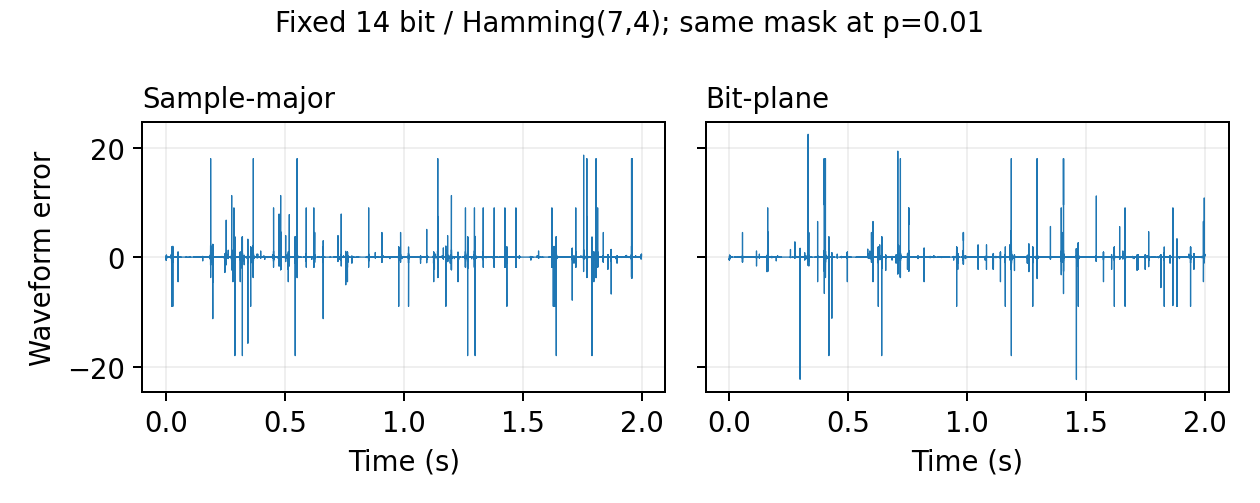
\includegraphics[width=.82\linewidth]{images/r51_packing_diagnostic.png}
 \caption{Same-mask waveform errors at $p=0.01$, Gaussian absent;
 quantiser, code, rate and axes fixed. One realisation illustrates packing,
 not expected gain.}
 \label{fig:r51-packing}
\end{figure}


Repetition gains $\RfiveRepeatGain $, interval
$[\RfiveRepeatLower,\RfiveRepeatUpper]$, but sends 1120 kbit/s and violates
the original twofold expansion rule. It cannot be a feasible winner.
Hamming(15,11) worsens the objective to $\RfiveCodeOtherJ $.
At $ p=0.1 $, exact block-failure laws give
$\RfiveQSeven/\RfiveQFifteen/\RfiveQRepeat $ for H74/H15/repetition
(Eq.~\eqref{eq:r51-block-failure}); both Hamming codes correct one
error, repetition two. Higher code rate is not stronger correction.
The 513-tap feasible filter worsens the objective and raises group delay
12 $\to $16 ms; other filter variants fail the original tone-gain guard.
No runtime penalty is inferred from their equal FFT length.

This scoped conclusion concerns nine variants and the chosen severity
weights, not a global optimum or real-world channel frequencies.
Gaussian error dominates personally; FIR distortion matters at 40 dB.
The R1--R4 baseline remains frozen; reflection does not retrospectively
substitute the 16 bit alternative into its validation.

\subsection{Change the code under a 320 kbit/s cap}
\label{sec:r52}
Under a declared logical cap 320 kbit/s, I choose Hamming(15,11),
retaining 16 kHz, 14 bit, $ A=18 $, the 385-tap FIR and both anchor parameters.
The scenario and its three means were frozen before the R5 pilot;
the same 350 confirmation records are reused, not new observations.
The cap is a project scenario for transmitting 2 s in 2 s, with rates measured as transmitted bits rather than physical energy. The threshold stays
$\tau=\SfiveThreshold $ from R3.4; neither applies to all stress conditions.

\begin{table}[htbp]
 \centering\small
 \caption{Exact 2 s costs under the new personal 320 kbit/s cap. Q fit retains the R3 quantisation budget; 11 bit is an analytic cost alternative, without new waveform measurements.}
 \label{tab:r52-cost}
 \begin{tabular}{lrrrrll}
\toprule
Scheme & Real bits & Pad & Sent bits & kbit/s & Rate fit & Q fit \\
\midrule
Hamming(7,4) & 448000 & 0 & 784000 & 392.00 & No & Yes \\
Hamming(15,11) & 448000 & 8 & 610920 & 305.46 & Yes & Yes \\
Uncoded & 448000 & 0 & 448000 & 224.00 & Yes & Yes \\
Repetition(5,1) & 448000 & 0 & 2240000 & 1120.00 & No & Yes \\
11 bit + (7,4) & 352000 & 0 & 616000 & 308.00 & Yes & No \\
\bottomrule
\end{tabular}

 
 
\end{table}

Exact framing (Eq.~\eqref{eq:r52-cost}) gives 40728 H15 codewords,
eight pad bits and 610920 transmitted bits, 305460 bit/s:
$\SfiveRateSaving $\% less traffic. Repetition exceeds the cap;
11 bit/H74 would fit at 308 kbit/s but its existing quantisation-budget
ratio $\SfiveBitElevenRatio>0.01 $ fails the retained requirement.
This is an analytic cost alternative, with no invented personal NMSE.

The unchanged acceptance rule requires both rate $\le320000 $ bit/s and
the 19-family approximate mean upper bound $\le\tau $
(Eq.~\eqref{eq:r52-quality}). An interval crossing $\tau $ is unresolved;
this rule is not a guarantee for each record.

\begin{table}[H]
 \centering\small
 \caption{Same 350 new R5 records at the anchor point. Intervals use the 19-statistic family; perfect payloads require all real information bits, excluding padding.}
 \label{tab:r52-quality}
 \begin{tabular}{lrrrl}
\toprule
Scheme & Mean NMSE [interval] & Payload BER & Perfect payloads & Mean rule \\
\midrule
Hamming(7,4) & 0.029145 [0.028931,0.029358] & $3.4439\times10^{-7}$ & 319/350 & Pass \\
Hamming(15,11) & 0.029279 [0.028995,0.029564] & $7.4617\times10^{-7}$ & 298/350 & Pass \\
Uncoded & 0.151197 [0.145161,0.157233] & $2.1117\times10^{-4}$ & 0/350 & Fail \\
\bottomrule
\end{tabular}

 
 
\end{table}

H15 mean $\SfiveNewMean $, upper bound $\SfiveNewUpper<\tau $, meets both.
H74 meets quality but exceeds the cap; uncoded fits rate but its mean
$\SfiveRawMean $ has lower bound above $\tau $. Both Hamming codes have
$ d_{\min}=3,t=1 $.
The gain in feasibility costs exact-payload reliability: perfect records
fall $\SfivePerfectBase/350\to\SfivePerfectNew/350 $ despite acceptable
mean waveform quality. Eq.~\eqref{eq:r52-payload} includes the H15 last
word's three real/eight padding bits; requiring correct padding would
test the wrong event. Unpadded H74 reduces to $(1-q_{7,1})^{112000}$;
uncoded to $(1-p)^{448000}$.
Pointwise Clopper--Pearson perfect-record intervals are separate from
the 19-family mean intervals (Eq.~\eqref{eq:r52-proportion-ci}).
Independent checks cover 1050 reused paths, 32898 error patterns and
exact costs. H15's worse main objective $\RfiveCodeOtherJ $ means this
personal cap-driven decision does not replace H74 for the original domain.

\FloatBarrier
\section{Stage 6: Integrity and reproducibility}
\subsection{Reproduce inputs, measurements and report}
\label{sec:r61}
The verified stack is Python 3.13.5, NumPy 2.1.3, SciPy 1.15.3,
Matplotlib 3.10.0 and Tectonic 0.17.0. The explicit Windows dependency
lock records the numerical and rendering environment. From the repository root:
\par\noindent\begin{minipage}{\linewidth}\small\begin{verbatim}
conda create -n signal-transmission --file conda-win-64-explicit.txt
conda activate signal-transmission
python run_all.py --tectonic PATH_TO_TECTONIC
\end{verbatim}\end{minipage}\par
\texttt{--data-only} skips PDF compilation. Worker settings and the
four-thread parameter scan are documented in \path{README.md}.

The entry point checks the NPY/WAV input hashes, then regenerates measured
CSV, figures and LaTeX fragments. It verifies \RsixProducts{} frozen
scientific targets plus seven packing-diagnostic products. CSV fields,
arrays, payloads and generated formula/table text are compared exactly;
raster comparisons use exact pixels. SVG comparisons retain geometry,
visible text and styling while excluding nonvisual export metadata and
consistently renamed opaque identifiers. The targets were fixed before
packaging and are never refreshed to conceal a mismatch. This release uses
the existing validated measurements; publication checks do not constitute
a new complete numerical replay.

\paragraph{Computational cross-checks.}
Alternative methods use direct convolution, midpoint and threshold
quantisation, XOR parity, correction-sphere lookup decoding and SciPy
resampling where applicable. Candidate kernels also have cosine-series
checks. These reproduce existing trials and do not add independent
observations. Complete records, rather than individual samples, are the
independent units in the reported uncertainty calculations.

The six final vector figures are regenerated automatically from measured
CSV by \path{reproduction/prepare_publication_figures.py}. A report-only
build uses \path{reproduction/build_pdf.py}. Two independent source-only
builds with a fixed \texttt{SOURCE\_DATE\_EPOCH} check deterministic PDF
output. Runtime evidence and scientific product hashes are saved under
\path{stage6/results/}. Exact replay is scoped to the recorded Windows
stack; execution on a second machine has not been tested.

\FloatBarrier
\begin{samepage}
\section*{Conclusions and limitations}
\phantomsection
\addcontentsline{toc}{section}{Conclusions and limitations}
\label{sec:conclusions}
For the supplied periodic multitone, the selected 16 kHz sampler retains
all identified components. The frozen 385-tap FIR, 14-bit quantiser and
Hamming(7,4) jointly give the lowest anchor-point mean NMSE,
$\WPersonalBoth$, and the lowest declared main-domain objective among
the four configurations. These are conditional results for the tested
signal, degradation models and severity weights. Increasing to 16 bits
improves the new R5 objective at greater traffic cost, while the separate
320 kbit/s anchor-point constraint favours Hamming(15,11) with reduced
perfect-payload reliability.

Statistical precision remains a limitation: seven of the 92 R4 means
miss the planned 5\% relative half-width, reaching \WMaxRelativePercent\%.
The 40 dB coded filter contrast includes zero and does not establish a
local ordering. Computational agreement does not remove this sampling
uncertainty. The reported intervals, high-SNR FIR distortion and finite
resource budgets delimit the conclusions; neither universal improvement
nor exact recovery of every payload is claimed.
\end{samepage}

\FloatBarrier
\begingroup
\small
\setlength{\bibsep}{0pt}
\interlinepenalty=10000
\renewcommand{\bibsection}{\section*{\refname}\phantomsection\addcontentsline{toc}{section}{\refname}}
\bibliographystyle{plainnat}
\bibliography{references}
\endgroup
\FloatBarrier
\clearpage
\appendix
\numberwithin{equation}{section}
\begingroup
\ReportAppendixStyle
\FloatBarrier
\Needspace{12\baselineskip}
\section{Selected parameters and evidence}
\label{sec:selected-parameters}
The frozen validation baseline is collected below; R5 alternatives retain
their own constraints (Sections~\ref{sec:r51}--\ref{sec:r52}). Full RNG
trial paths are in \path{metadata/randomness_design.json}.
\begingroup
\normalsize
\setlength{\tabcolsep}{4.5pt}
\setlength{\extrarowheight}{2pt}
\renewcommand{\arraystretch}{1.22}
\setlength{\LTcapwidth}{0.94\linewidth}
\begin{longtable}{p{0.22\linewidth}p{0.46\linewidth}p{0.25\linewidth}}
\caption{Frozen baseline and selection evidence. SNR/$p$ mappings are
declared project choices, not a supplied external conversion.}
\label{tab:selected-parameters}\\
\toprule
Parameter & Selected value & Evidence\\\midrule
\endfirsthead
\multicolumn{3}{c}{Table~\thetable\ continued}\\\toprule
Parameter & Selected value & Evidence\\\midrule
\endhead
\bottomrule\endfoot
Source / sampling & 48 kHz, 96000 samples $\to$ $\TransmissionRate$ Hz,
 $\TransmissionCount$ samples; 2 s; unmodified NPY units
 & Section~\ref{sec:r11}; Tables~\ref{tab:components}, \ref{tab:rates}\\
RNG / purpose streams & Root 2470964; PCG64; SeedSequence pool size 4;
 parameters 0, Gaussian 1, BSC 2
 & Anchor-seed convention; Sections~\ref{sec:r21}, \ref{sec:r33}, \ref{sec:r42}\\
Personal degradation & SNR $\RtwoPersonalSnr$ dB from $[0,30]$ dB;
 $p_{\rm ID}=\PPersonal$ from $[10^{-4},0.1)$
 & Eq.~\eqref{eq:r21-personal-snr}; Table~\ref{tab:r33-range}\\
FIR centres & 440, 1320, 2200, 6000 Hz
 & Tables~\ref{tab:components}, \ref{tab:r22-spectrum}\\
FIR design & $\RttLength$ symmetric \RttWindow{} taps;
 centre $\pm\RttHalfWidth$ Hz and conjugate negative bands
 & Table~\ref{tab:r22-windows}; Figures~\ref{fig:r22-search}, \ref{fig:r22-response-boundary}\\
FIR implementation / delay & Zero-extended linear FFT convolution,
 $K=\RttFFT$, fixed centre crop; $\RttDelay$ samples,
 $\RttDelayMs$ ms causal delay
 & Eq.~\eqref{eq:r21-padded-convolution}; Sections~\ref{sec:r22}--\ref{sec:r23}\\
Quantiser / rounding & $B=\QBits$, $A=\QHalfRange$, $\QLevels$ endpoint
 levels; $\Delta=\QStep$; shifted round-to-even, $\epsilon=10^{-9}$,
 saturation
 & Eq.~\eqref{eq:r31mapping}; Table~\ref{tab:r31bits}; exhaustive label checks\\
Bit budget / packing & Quantisation component at most 1\% of upstream
 error power; unsigned natural binary, sample-major, MSB first
 & Eq.~\eqref{eq:r31budget}; Section~\ref{sec:r31}; label round trips\\
ECC / payload / rate & Systematic Hamming(7,4), $d_{\min}=3$, $t=1$;
 448000 information / 784000 sent bits; no padding; 392 kbit/s
 & Eq.~\eqref{eq:r32-matrices}; Table~\ref{tab:r32-selection}; Eq.~\eqref{eq:r32-framing}\\
Reconstruction & Periodic Fourier interpolation to all 96000 original
 positions
 & Eq.~\eqref{eq:periodic-interpolation}; R1 and cross-grid checks\\
Primary metric & Whole-record NMSE; reference power $\MReferencePower$
 & Section~\ref{sec:r41}; Figure~\ref{fig:r41-ranking}\\
Quality threshold & $\tau=\CTau$; fixed before validation
 & Eq.~\eqref{eq:r34-budget}; Table~\ref{tab:r34-quality}\\
\end{longtable}
\endgroup
\FloatBarrier

\clearpage
\setlength{\parskip}{2.5pt}
\setlength{\abovedisplayskip}{5pt}
\setlength{\belowdisplayskip}{5pt}
\setlength{\belowdisplayshortskip}{3pt}
\renewcommand{\arraystretch}{1.05}
\section{Formula derivations and implementation conventions}
\label{app:derivations}
Shared formulas are derived once, with explicit assumptions and published technical references.
Finite-array consequences are derived here; statistical methods and design
preferences are supplementary. Symbols are local: $N$ is a sampled record
length, $L$ the reference/reconstruction length, $K$ a transform length and
$L_q=2^B$ the number of quantiser levels. Powers specify their grid.
Receiver algorithms use no reference waveform or true channel errors.

\subsection{Finite-record Fourier, windows and power}
\label{app:dft}
\paragraph{DFT pair and one-sided scaling.}
Use the unscaled forward transform and $1/L$ inverse:
\begin{align}
 X[k]&=\sum_{n=0}^{L-1}x[n]e^{-j2\pi kn/L},\quad
 f_k=\frac{kF_0}{L},\quad\Delta f=\frac{F_0}{L}=\BinSpacing\,\mathrm{Hz},
 \label{eq:r11-dft}\\
 x[n]&=\frac1L\sum_{k=0}^{L-1}X[k]e^{j2\pi kn/L}.
 \label{eq:inverse}
\end{align}
Euler's cosine pair, $A\cos\theta=(A/2)(e^{j\theta}+e^{-j\theta})$,
gives, for an isolated coherent interior component,
\begin{equation}
 x[n]=A\cos(2\pi k_0n/L+\phi)
 \quad\Longrightarrow\quad X[k_0]=\tfrac{LA}{2}e^{j\phi}.
 \label{eq:cosine-amplitude}
\end{equation}
For $N$ actual samples and even $K\ge N$, the general windowed scales are

\begin{align}
 Y_{a,K}[k]&=\sum_{n=0}^{N-1}y[n]a[n]e^{-j2\pi kn/K},\quad
 f_k=\frac{kf_s}{K},\nonumber\\
 A_{a,K}[k]&=\frac{c_k|Y_{a,K}[k]|}{\sum_na[n]},\quad
 \widehat S_{a,K}[k]=\frac{c_k|Y_{a,K}[k]|^2}{f_s\sum_na[n]^2}.
 \label{eq:r22-spectrum-scales}
\end{align}
Here $c_k=1$ at DC/Nyquist and 2 at other positive bins. For $N=K=L$,
write $X_w=Y_{w,L}$ and $CG=L^{-1}\sum_nw[n]$; thus
$\widehat A_w=c_k|X_w|/(L\,CG)$. With $W=\operatorname{DFT}_L(w)$,
substitution of the cosine pair yields
\begin{equation}
 X_w[k_0]=\tfrac A2e^{j\phi}W[0]+\tfrac A2e^{-j\phi}W[2k_0],
 \qquad W[0]=L\,CG.
 \label{eq:window-gain-derivation}
\end{equation}
Normalising the first term does not remove mirror, off-bin or overlapping
components. Padding changes $\Delta f_K=f_s/K$, not the window-sum denominators.

\paragraph{Orthogonality, Parseval and PSD.}
For DFT indices $k,\ell\in\{0,\ldots,L-1\}$, the geometric ratio
$r=e^{j2\pi(k-\ell)/L}$ gives $(1-r^L)/(1-r)=0$ when $k\ne\ell$.
Insert the IDFT, cancel unequal-index terms, then pair conjugate bins:
\begin{align}
 \sum_{n=0}^{L-1}e^{j2\pi(k-\ell)n/L}&=L\delta_{k\ell},
 \label{eq:finite-orthogonality}\\
 \sum_n|x[n]|^2
 &=\frac1{L^2}\sum_{k,\ell}X[k]X^*[\ell]L\delta_{k\ell}
 =\frac1L\sum_k|X[k]|^2,\label{eq:parseval-steps}\\
 P_k&=c_k\frac{|X[k]|^2}{L^2},\qquad
 \widehat P=L^{-1}\sum_nx[n]^2=\sum_{k=0}^{L/2}P_k.
 \label{eq:parseval}
\end{align}
Applying the same identity to the padded windowed record gives
\begin{equation}
 \sum_{k=0}^{K/2}\widehat S_{a,K}[k]\frac{f_s}{K}
 =\frac{\sum_{k=0}^{K-1}|Y_{a,K}[k]|^2}{K\sum_na[n]^2}
 =\frac{\sum_ny[n]^2a[n]^2}{\sum_na[n]^2}.
 \label{eq:r22-psd-integral}
\end{equation}
PSD has squared NPY-amplitude/Hz units. Its weighted integral need not equal
the raw signal power used for noise generation.

\paragraph{Shared symmetric windows.}
For length $M$, $0\le n<M$, the tested windows are
\citep{numpy21hanning,numpy21hamming}
\begin{equation}
 \theta_n=\frac{2\pi n}{M-1},\quad w_{\rm rect}=1,\quad
 w_{\rm Hann}=\tfrac12(1-\cos\theta_n),\quad
 w_{\rm Hamming}=0.54-0.46\cos\theta_n.
 \label{eq:r22-windows}
\end{equation}
The spectral Hann $w_H$ uses $M=L$; kernel tapers use the FIR length.

\subsection{Sampling, interpolation and aliasing}
\label{app:sampling}
\paragraph{Folding and periodic recovery.}
For decimation $L=MN$, substitute $x_{\rm ref}[Mm]$ from the IDFT.
Orthogonality retains only $r=k+qN$, including phase:
\begin{equation}
 \frac{Y[k]}N=\frac1{LN}\sum_{r=0}^{L-1}X[r]
 \sum_{m=0}^{N-1}e^{j2\pi(r-k)m/N}
 =\sum_{q=0}^{M-1}\frac{X[k+qN]}L,\quad0\le k<N.
 \label{eq:decimation-folding}
\end{equation}
For real even-$N$ data, $Y=\operatorname{DFT}_N(x_M)$. Pairing the reference
IDFT and evaluating at $t/T=n/L$ gives the periodic interpolator:
\begin{equation}
 \widehat x[n]=\frac1N\left[Y[0]
 +2\operatorname{Re}\sum_{k=1}^{N/2-1}Y[k]e^{j2\pi kn/L}
 +Y[N/2]\cos\!\left(\frac{\pi Nn}{L}\right)\right].
 \label{eq:periodic-interpolation}
\end{equation}
For \texttt{irfft(Z,L)}, $L>N$, the old Nyquist coefficient splits into
an interior conjugate pair, requiring
\begin{equation}
 Z[k]=\frac LN Y[k]\ (k<N/2),\quad
 Z[N/2]=\frac L{2N}Y[N/2],\quad Z[k]=0\ (k>N/2).
 \label{eq:interpolation-scaling}
\end{equation}
For $L=N$ it is not split. DC/phased/Nyquist tests and independent SciPy
resampling check the convention \citep{numpy21irfft,scipy1153resample}.
The measured two-second periodicity supports this ideal-baseband recovery. Its inputs are only the samples and
target length; it does not recover arbitrary nonperiodic records.

\paragraph{Boundary phase and signed aliases.}
At $f_0=f_s/2$, the unknown sine component is lost:
\begin{equation}
 A\cos(\pi m+\phi)=A(-1)^m\cos\phi.
 \label{eq:critical-phase}
\end{equation}
For nonboundary $f_d=f_0-qf_s\in(-f_s/2,f_s/2)$, $f_d\ne0$, and $f_a=|f_d|$,
\begin{equation}
 A\cos(2\pi f_0m/f_s+\phi)=A\cos(2\pi f_am/f_s+\phi_a),\qquad
 \phi_a=\operatorname{sgn}(f_d)\phi.
 \label{eq:alias-phase}
\end{equation}
In the 8~kHz diagnostic, the retained low-frequency terms cancel, leaving
\begin{equation}
 e_8(t)\simeq-0.1\sin(2\pi\,2000t)-0.1\sin(2\pi\,6000t).
 \label{eq:alias-error-model}
\end{equation}
These distinct integer-bin tones are orthogonal on the common grid, so
\begin{equation}
 \mathrm{MSE}_{8,\rm pred}=0.1^2/2+0.1^2/2=0.01.
 \label{eq:alias-error-power}
\end{equation}
This explains measured phases after the experiment; no source tones enter
the recovery algorithm.

\subsection{Linear filtering, finite boundaries and reconstruction energy}
\label{app:filter}
\paragraph{Convolution and padding.}
The reference impulse expansion $y[n]=\sum_my[m]\delta[n-m]$, linearity
and time invariance give 
\begin{equation}
 z[n]=\mathcal T\{y\}[n]=\sum_my[m]\mathcal T\{\delta[\cdot-m]\}[n]
 =\sum_my[m]h[n-m].
 \label{eq:r21-lti-convolution}
\end{equation}
For circular convolution, $r=(n-m)\bmod K$ separates the DFT sum:
\begin{equation}
 Z_c[k]=\sum_mh[m]e^{-j2\pi km/K}\sum_ry[r]e^{-j2\pi kr/K}
 =H_K[k]Y_K[k].
 \label{eq:r21-convolution-theorem}
\end{equation}
Zero extension gives $N+M-1$ full outputs. Linear convolution is therefore
\begin{equation}
 z_K[n]=\frac1K\sum_{k=0}^{K-1}H_K[k]Y_K[k]e^{j2\pi kn/K},
 \qquad K\ge N+M-1.
 \label{eq:r21-padded-convolution}
\end{equation}
retaining the first $N+M-1$ values, with zero padding.
The 513-tap prototype has 32512 full outputs; $K=32768$ is convenient,
not a NumPy requirement. An insufficient-padding counterexample is

\begin{equation}
 [1,2,1]*[2,0,2]=[2,4,4,4,2],
 \qquad
 \operatorname{IDFT}_4(Y_4H_4)=[4,4,4,4].
 \label{eq:r21-wrap-example}
\end{equation}
A centred three-point mean has aligned response
\begin{equation}
 h=[1,1,1]/3,\quad d=1,\qquad
 G_3(\omega)=e^{j\omega d}\sum_{m=0}^2h[m]e^{-j\omega m}
 =\frac{1+2\cos\omega}{3}.
 \label{eq:r21-ma-response}
\end{equation}

\paragraph{One finite-IDFT filter family.}
For signed frequencies $f_k$, measured corrupted-spectrum centres $f_i$,
half-width $b$, odd $M$ and $d=(M-1)/2$,

\begin{align}
 B_b[k]&=\mathbf1\!\left\{\min_i\bigl||f_k|-f_i\bigr|\le b\right\},\\
 h_{M,b,w}[m]&=w[m]\frac1N\sum_{k=0}^{N-1}
 B_b[k]e^{j2\pi k(m-d)/N},\qquad d=(M-1)/2.
 \label{eq:r22-family}
\end{align}
Use the symmetric windows in Eq.~\eqref{eq:r22-windows} on the kernel,
$0\le m<M$. The Hann prototypes use 513 taps and 80~Hz half-width in R2.1,
then 385 taps and 70~Hz in R2.2. The low-pass comparator uses
$B_b=\mathbf1_{\{|f_k|\le6600\,\mathrm{Hz}\}}$.
This project construction uses the declared R1 priors, not true noise.
The realised response is $\operatorname{DFT}_K(h)$, not the binary template.

With zero extension, the reference-independent crop is
\begin{equation}
 \widehat x[n]=z_{\rm full}[n+d],\quad 0\le n<N.
 \label{eq:r21-centred-crop}
\end{equation}
The offline crop uses future samples; causal FIR delay is $d/f_s$
(16~ms for the prototype), distinct from whole-record FFT buffering.

\paragraph{Finite-boundary noise gain, distortion and crossover.}
For a fixed filter, write $d_x=F(x)-x$, $v=F(e)$ and $y=x+e$:
\begin{equation}
 F(y)-x=d_x+v,\qquad
 \mathrm{MSE}=(\|d_x\|^2+\|v\|^2+2d_x^{\mathsf T}v)/N.
 \label{eq:r22-distortion-decomposition}
\end{equation}
For new independent zero-mean noise, $g[\ell]=h[\ell+d]$, $d<N$,
each lag overlaps $N-|\ell|$ positions. Thus
\begin{align}
 G_{\rm finite}&=\sum_{\ell=-d}^dg[\ell]^2(1-|\ell|/N),\nonumber\\
 \mathbb E[\mathrm{MSE}]&=D+\sigma^2G_{\rm finite},\qquad D=\|d_x\|^2/N.
 \label{eq:r22-finite-noise-gain}
\end{align}
The cross term vanishes in expectation, not in each trial. For $D>0,G<1$,
$D+\sigma^2G=\sigma^2$ gives $\sigma^2=D/(1-G)$ and
\begin{equation}
 S_* =10\log_{10}\frac{P_x(1-G_{\rm finite})}{D}
       \approx\RttCrossover\ {\rm dB}.
 \label{eq:r22-crossover}
\end{equation}

\paragraph{Reconstruction-grid energy and expected noise.}
For the frozen filter, $D=\RttCleanMse$ and $G=\RttNoiseGain$ in
Eq.~\eqref{eq:r22-finite-noise-gain}. Let $V=\operatorname{DFT}_N(v)$ for
a real even-$N$ error vector and $A_\pi=V[N/2]/N=N^{-1}\sum_n(-1)^nv[n]$.
For interpolation $R$ to $L=3N$, ordinary pairs retain their mean-square
contribution; splitting the old Nyquist coefficient halves its power:
\begin{align}
 \frac1N\|v\|^2
 &=\frac{|V[0]|^2+
 2\sum_{k=1}^{N/2-1}|V[k]|^2+|V[N/2]|^2}{N^2},\nonumber\\
 \frac1L\|R(v)\|^2
 &=\frac{|V[0]|^2+
 2\sum_{k=1}^{N/2-1}|V[k]|^2+\tfrac12|V[N/2]|^2}{N^2}\nonumber\\
 &=\frac1N\|v\|^2-\frac12 A_\pi^2.
 \label{eq:r23-reconstruction-energy}
\end{align}
With $a_n=(-1)^n/N$, independence gives
$\mathbb E[(a^{\mathsf T}Fe)^2]=\sigma^2\|F^{\mathsf T}a\|^2$, so
\begin{equation}
 G_{48}=G-\frac12\|F^\mathsf{T}a\|^2
       =\RtvNoiseGainHigh,\qquad
 G_{0,48}=1-\frac1{2N}=0.999984375.
 \label{eq:r23-high-gain}
\end{equation}
The 48~kHz predictions are $D_{48}+\sigma^2G_{48}$ and
$\sigma^2G_{0,48}$, with measured clean distortion $D_{48}=\RtvCleanHigh$;
negligible clean interpolation residuals are omitted. Actual errors use
the original reference, rather than assuming the two grids are equivalent.

\paragraph{Independent finite cosine-series kernel.}
For disjoint interior bands centred on DFT bins, integer $J_b=bN/f_s$
and $C_b=2J_b+1$, the finite geometric series gives an independent check:
\begin{align}
 S_{C_b}(\ell)
 &=\sum_{q=-J_b}^{J_b}e^{j2\pi q\ell/N}
 =\begin{cases}
 C_b,&\ell=0,\\
 \dfrac{\sin(C_b\pi\ell/N)}{\sin(\pi\ell/N)},&\ell\ne0,
 \end{cases}\nonumber\\
 h[m]&=\frac{2w[m]}{N}S_{C_b}(m-d)
       \sum_i\cos\!\left(\frac{2\pi f_i(m-d)}{f_s}\right).
 \label{eq:r23-audit-kernel}
\end{align}

\subsection{Quantisation, binary labels and amplitude errors}
\label{app:quant}
\paragraph{Endpoint codebook and shifted rounding.}
The endpoint mapping, Eq.~\eqref{eq:r31mapping}, has spacing
$\Delta=2A/(L_q-1)$ versus the ideal-model $2A/L_q$. The normalised epsilon
shifts rounding by $A\epsilon$, giving $|z_q-z_c|\le\Delta/2+A\epsilon$
apart from floating-point effects. The even endpoint codebook omits zero;
the retained shift maps zero to $-\Delta/2$. With clipping,
$e_q=(z_c-z)+(z_q-z_c)$, whose power includes their cross term.
Actual errors need not be white, independent or zero-mean
\citep{widrow1996quantization}.

\paragraph{Common headroom and an overload bound.}
Both branches share a range fixed before noise generation for the
$-10$ to 40~dB stress envelope. Let $M_b=\max_n|F_b(x)[n]|$,
$g_0=1$, $g_F=\|h\|_2$ and
$\sigma_{\max}=\sqrt{P_x10^{-S_{\min}/10}}=2.701851$ at $S_{\min}=-10$~dB.
Independence gives $\operatorname{Var}[(F\eta)[n]]
\le\sigma^2\|h\|_2^2$, including boundaries. Six-sigma headroom yields
\begin{equation}
 A=\left\lceil\max_b(M_b+6\sigma_{\max}g_b)\right\rceil
 =\left\lceil\max(\QRawHeadroom,\QFilterHeadroom)\right\rceil=\QHalfRange.
 \label{eq:r31range}
\end{equation}
For unbounded Gaussian noise this is not a zero-overload guarantee:
$\Pr(\text{any overload})\le2N\operatorname{erfc}(6/\sqrt2)=\QUnionBound$
for the two $N=32000$ branches by the union bound, without branch
independence. Overloads are counted before clipping; the stress envelope
does not expand R2's design claims.

\paragraph{Uniform-error integral and SQNR conventions.}
The reference's unoverloaded model has $p_e(e)=1/\Delta$ on
$[-\Delta/2,\Delta/2)$ and $\mathbb E[e]=0$ by symmetry. Its model variance is
\citep{bennett1948spectra}
\begin{equation}
 \mathbb E[e^2]=\frac1\Delta\int_{-\Delta/2}^{\Delta/2}e^2\,de
 =\frac1\Delta\left[\frac{e^3}3\right]_{-\Delta/2}^{\Delta/2}
 =\frac{\Delta^2}{12}.
 \label{eq:r31variance}
\end{equation}
For endpoint spacing and $R_a=2A$, this gives the model
\begin{equation}
 {\rm SQNR}_{\rm model}
 =10\log_{10}\!\left(\frac{12P_z}{\Delta^2}\right)
 =10\log_{10}\!\left(\frac{12P_z(2^B-1)^2}{R_a^2}\right).
 \label{eq:r31model}
\end{equation}
A full-range sine has $P_z=R_a^2/8$, so the ideal uniform spacing gives
$10\log_{10}(1.5\,4^B)=10\log_{10}1.5+20B\log_{10}2
\simeq1.76+6.02B$~dB. Endpoint spacing adds $20\log_{10}(1-2^{-B})$.
Neither sine formula is the actual multitone/noisy-input SQNR.

\paragraph{Random-label power and the p=0.5 full-grid check.}
At $p=0.5$, received bits are independent fair bits, independent of the
payload. Hamming(7,4)'s 16 equal eight-word correction spheres give uniform
decoded messages, hence independent fair information bits and uniform
disjoint 14-bit labels. For uniform $j\in\{0,\ldots,L_q-1\}$,
$\mathbb E[j]=(L_q-1)/2$ and $\operatorname{Var}(j)=(L_q^2-1)/12$, giving
\begin{equation}
 V_q=\left(\frac{2A}{L_q-1}\right)^2\operatorname{Var}(j)
 =\frac{A^2(L_q+1)}{3(L_q-1)}.
 \label{eq:r43-uniform-label}
\end{equation}
Here $A=18,L_q=2^{14}$. This is decoded-level power, not $\Delta^2/12$.
The reference cross term has zero expectation; Nyquist correction gives
\begin{equation}
 \mathbb E[d\mid p=0.5]
 =1+\frac{V_q}{P_{\rm ref}}\left(1-\frac1{2N}\right)
 =\WHalfTheory,\qquad N=32000.
 \label{eq:r43-half-theory}
\end{equation}

\paragraph{Bit depth, label significance and code-block coupling.}
The endpoint model predicts only the quantisation-component ratio
\begin{equation}
 \frac{P_{q,16}}{P_{q,14}}
 =\left(\frac{2^{14}-1}{2^{16}-1}\right)^2\simeq\frac1{16},
 \label{eq:r51-quant-ratio}
\end{equation}
For true MSB-first bits $b_{n,u}$ and error indicators $w_{n,u}$, XOR is
$\widehat b_{n,u}=b_{n,u}+(1-2b_{n,u})w_{n,u}$. Therefore
\begin{equation}
 \begin{aligned}
 \ell[n]&=\sum_{u=0}^{B-1}2^{B-1-u}b_{n,u},\quad z_q[n]=-A+\Delta_B\ell[n],\\
 \delta z[n]&=\Delta_B(\widehat\ell[n]-\ell[n])
 =\Delta_B\sum_{u=0}^{B-1}(1-2b_{n,u})2^{B-1-u}w_{n,u}.
 \end{aligned}
 \label{eq:r51-bit-coupling}
\end{equation}
At $B=14$, one MSB error has $2^{13}$ times an LSB error's amplitude
magnitude and $2^{26}$ times its squared magnitude. Squaring retains joint
$w_{n,u}w_{n,v}$ terms. Label starts $(Bn)\bmod4$ alternate 0/2 for 14 bits
but stay 0 for 16; dependent within-codeword errors therefore interact
differently with significant bits. Component/cross-term measurements capture
the combined change, not an isolated alignment effect or resolution-only gain.

\paragraph{Fixed-resolution packing diagnostic.}
With fixed 14-bit labels, $\alpha_{n,u}=\Delta 2^{13-u}(1-2b_{n,u})$.
Let $A_b$ place codeword $b$'s four slopes in their sample positions:
$\delta z=\sum_bA_bw_b$. The 128 BSC patterns give residual-bit mean $q$
and covariance $C$. Independent blocks give
$m=\mathbb E[\delta z]=\sum_bA_bq$ and
$\Sigma=\operatorname{Cov}(\delta z)=\sum_bA_bCA_b^T$.
Apply Eq.~\eqref{eq:r23-reconstruction-energy} to the zero-mean fluctuation:
\begin{equation}
 \mathbb E[d]=\frac{1}{P_{\rm ref}}\left\{
 \frac{\|\mathcal R(z_q+m)-x_{\rm ref}\|^2}{L}
 +\frac{\operatorname{tr}\Sigma}{N}
 -\frac{a^T\Sigma a}{2N^2}\right\},\quad a_n=(-1)^n.
 \label{eq:packing-expectation}
\end{equation}
The final term corrects split Nyquist energy. Packing changes $A_b$,
with $q,C,z_q$ fixed; Gaussian is absent. The code accumulates block
moments without storing $\Sigma$.

\subsection{Systematic ECC, channel error laws and payload counting}
\label{app:ecc}
Counting fixed-width samples gives
\begin{equation}
 R_{\mathrm{raw}}=Bf_s,\qquad N_{\mathrm{bits}}=BN,\qquad
 \frac{R_{\mathrm{raw},i}}{R_{\mathrm{raw},16k}}=\frac{f_{s,i}}{16000}.
 \label{eq:sampling-payload}
\end{equation}

\paragraph{Fixed matrices, syndrome, distance and miscorrection.}
The reference distance and correction radius are

\begin{align}
 d_H(\mathbf u,\mathbf v)&=\sum_{i=0}^{n-1}
       \mathbb{1}\{u_i\ne v_i\},&
 d_{\min}&=\min_{\mathbf u\ne\mathbf v\in C}d_H(\mathbf u,\mathbf v),
 \label{eq:r32-distance}\\
 R&=\frac{k}{n},&
 t&=\left\lfloor\frac{d_{\min}-1}{2}\right\rfloor.
 \label{eq:r32-rate}
\end{align}
A validity check detects up to $d_{\min}-1$ errors; correction guarantees
only $t$. All arithmetic is in $\mathrm{GF}(2)$, using integer NumPy
matrix multiplication modulo two over GF(2). The actual row-message matrices are

\begin{equation}
 G_7=\left[\begin{array}{rrrr|rrr}
 1&0&0&0&1&1&0\\0&1&0&0&1&0&1\\
 0&0&1&0&0&1&1\\0&0&0&1&1&1&1
 \end{array}\right],\qquad
 H_7=\left[\begin{array}{rrrr|rrr}
 1&1&0&1&1&0&0\\1&0&1&1&0&1&0\\0&1&1&1&0&0&1
 \end{array}\right].
 \label{eq:r32-matrices}
\end{equation}
For $G=[I_k\mid P]$ and $H=[P^T\mid I_{n-k}]$,
\begin{equation}
 GH^T=P+P=0,\quad \mathbf c=\mathbf mG,\quad
 \mathbf r=\mathbf c+\mathbf e,\quad
 \mathbf s=\mathbf rH^T=\mathbf eH^T.
 \label{eq:r32-syndrome}
\end{equation}
A single-error syndrome equals the corresponding column of $H$.
Its columns, in order, are 110, 101, 011, 111, 100, 010, 001.
Use column matching rather than binary-syndrome indexing;
zero syndrome leaves the word unchanged. Extract the first $k$ bits
after correction.
The reference example $1100\mapsto1100011$ becomes $1110011$ after flipping
zero-based position 2; syndrome $011$ restores it. Enumeration of all 16
messages gives minimum nonzero weight 3. Linearity,
$d_H(c_1,c_2)=w_H(c_1+c_2)$, proves $d_{\min}=3$.
The disjoint radius-one spheres contain $2^4(1+7)=2^7$ words, a perfect
partition; sphere size alone is not proof of correction.

Two flips $0000000\to1100000$ also give syndrome $011$: correction produces
the wrong valid word $1110000$, message $1110$, with final syndrome zero.
This decoder is not SECDED; validity does not prove message recovery.

\paragraph{Alternative codes and majority decoding.}
For the $(15,11)$ reference code, define $G_{15}=[I_{11}\mid P_{15}]$ and
$H_{15}=[P_{15}^T\mid I_4]$ by these ordered four-bit parity rows:
\begin{equation}
 \begin{aligned}
 \operatorname{rows}(P_{15})={}&(1100,1010,1001,0110,0101,0011,\\
 &1110,1101,1011,0111,1111).
 \end{aligned}
 \label{eq:r32-p15}
\end{equation}
Each string is one binary row. Distinct nonzero columns of $H_{15}$ exclude
weight-one/two codewords; the first generator row has weight three.
Thus $d_{\min}=3,t=1,R=11/15$. The five-repetition reference alternative has
$G_5=[1\ 1\ 1\ 1\ 1]$, $H_5=[\mathbf1_4\mid I_4]$,
$d_{\min}=5,t=2,R=1/5$. Majority fails on three or more flips:
\begin{equation}
 P_{b,5}=10p^3(1-p)^2+5p^4(1-p)+p^5.
 \label{eq:r32-repeat}
\end{equation}
The ideal-model three-repetition example instead gives $3p^2-2p^3$. Uncoded $(1,1)$ has
$d_{\min}=1,t=0,R=1,P_b=p$.

\paragraph{Exact framing, padding and effective rate.}
For $N$ labels of $B$ bits, duration $T$ and an $(n,k)$ code,
\begin{align}
 M_b&=NB,\qquad a=(-M_b)\bmod k,\qquad
 N_c=\left\lceil M_b/k\right\rceil,\nonumber\\
 M_t&=nN_c,\qquad R_{\mathrm{eff}}=M_b/M_t,\qquad r_t=M_t/T.
 \label{eq:r32-framing}
\end{align}
Here $N=32000,B=14,T=2$~s, so $M_b=448000$. R3.2 also uses $M=M_b,v_t=r_t$.
The last word has $b=M_b-k(N_c-1)$ real bits. Padding is encoded and counted
in the logical sending rate but excluded from real-payload BER; headers
and physical energy lie outside this rate definition.

Independent BSC flips imply
\begin{equation}
 E_i\overset{\mathrm{iid}}{\sim}\operatorname{Bernoulli}(p),\quad
 J_b=\sum_{i=1}^n E_i\sim\operatorname{Binomial}(n,p),\quad
 \Pr(J_b=j)=\binom njp^j(1-p)^{n-j}.
 \label{eq:r32-binomial}
\end{equation}

\paragraph{Exact complete-block failure and decoded BER.}
For the verified perfect Hamming and odd-repetition decoders, complete
padded-message failure occurs exactly when error weight exceeds $t$:
\begin{equation}
 q_{n,t}(p)=1-\sum_{j=0}^t\binom njp^j(1-p)^{n-j}
 =\sum_{j=t+1}^n\binom njp^j(1-p)^{n-j}.
 \label{eq:r32-bler}
\end{equation}
The positive tail is numerically stable. This law is not assumed for
arbitrary ECC; real-payload BER excludes Hamming(15,11)'s eight padding bits.
Translation invariance, Eq.~\eqref{eq:r42-pair-invariant}, permits all-zero
message enumeration. Grouping patterns by weight gives
\begin{equation}
 \begin{aligned}
 A_{c,j}&=\sum_{\mathbf e:\,w_H(\mathbf e)=j}w_H(\mathcal D_c(\mathbf e)),\\
 P_{b,c}(p)&=\frac1k\sum_{j=0}^n A_{c,j}p^j(1-p)^{n-j}.
 \end{aligned}
 \label{eq:r32-exactber}
\end{equation}
Multiplicity is included in $A_{c,j}$. The (7,4) coefficients
$(0,0,36,76,64,48,28,4)$ give $P_b=9p^2+O(p^3)$; (15,11) gives
$21p^2+O(p^3)$. Also $q_{7,1}=1-(1-p)^7-7p(1-p)^6=21p^2+O(p^3)$.

\paragraph{Capacity and rate are distinct from finite-code error.}
The memoryless BSC capacity is
\begin{equation}
 H_2(p)=-p\log_2p-(1-p)\log_2(1-p),\qquad C(p)=1-H_2(p),
 \label{eq:r33-capacity}
\end{equation}
Use $0\log_20=0$; $C(p)=4/7$ gives $p=\PCapacityRoot$.
Capacity does not predict this finite decoder's BER.

\paragraph{Exact finite-code BER crossover.}
Expanding the (7,4) enumerator and factoring gives the nontrivial
crossover in $(0,1/2)$:
\begin{align}
 P_{b,7}(p)&=9p^2-26p^3+30p^4-12p^5,\nonumber\\
 P_{b,7}(p)-p&=-p(2p-1)(p-1)(6p^2-6p+1),\label{eq:r33-bercross}\\
 p_{\rm BER}&=(3-\sqrt3)/6=\PBerRoot.\label{eq:r33-berroot}
\end{align}

\paragraph{Decoder invariance under a shared mask.}
Adding a valid codeword leaves syndrome and correction vector
$\kappa(\mathbf s)$ unchanged. For information projection $\pi_4$,
\begin{equation}
 \mathbf s=(\mathbf c\oplus\mathbf e)H^T=\mathbf eH^T,\qquad
 D_1(E_1(\mathbf b)\oplus\mathbf e)
 =\mathbf b\oplus\pi_4[\mathbf e\oplus\kappa(\mathbf eH^T)].
 \label{eq:r42-pair-invariant}
\end{equation}
Hence $\mathcal D(c\oplus e)=m\oplus\mathcal D(e)$; odd-repetition majority
has the same translation property. The same mask gives identical decoded
error patterns across messages.

\paragraph{Exact real-payload probability with a partial final word.}
Let $b=M_b-(N_c-1)k$ and let $a_{b,w}$ count weight-$w$ patterns whose
decoded first $b$ bits remain correct. Translation invariance and independent
disjoint BSC words give
\begin{align}
 s_b(p)&=\sum_{w=0}^n a_{b,w}p^w(1-p)^{n-w},\label{eq:r52-prefix}\\
 P_{\rm exact\ payload}
 &=(1-q_{n,t}(p))^{N_c-1}s_b(p).\label{eq:r52-payload}
\end{align}
For (15,11), $b=3$ and eight bits are padding, so
$(1-q_{15,1})^{40728}$ is not exact real-payload recovery.
For unpadded (7,4), $b=4$, $s_b=1-q_{7,1}$, yielding
$(1-q_{7,1})^{112000}$; uncoded transmission gives $(1-p)^{448000}$.

\subsection{Reconstruction metrics and error accounting}
\label{app:metrics}
\paragraph{Common finite-record metrics and units.}
For reference $u$, recovery $\widehat u$, $Q$ grid positions and $P_u>0$,
\begin{equation}
 \begin{aligned}
 a[j]&=\widehat u[j]-u[j],\quad P_u=Q^{-1}\sum_ju[j]^2,\quad
 E=\operatorname{MSE}=Q^{-1}\sum_ja[j]^2,\\
 \operatorname{RMSE}&=\sqrt E,\qquad \operatorname{NMSE}=E/P_u,\qquad
 S_{\rm error}=10\log_{10}(P_u/E).
 \end{aligned}
 \label{eq:r23-metrics}
\end{equation}

Cauchy--Schwarz gives
\begin{equation}
 \operatorname{MAE}=Q^{-1}\sum_j|a[j]|\leq
 \sqrt{Q^{-1}\sum_ja[j]^2}=\operatorname{RMSE}.
 \label{eq:r41-mae}
\end{equation}
MAE is not a monotone transform of MSE.

For paired repeat $r$,
\begin{equation}
 \delta_r=E_{0,r}-E_{F,r},\qquad
 g_r=S_{{\rm error},F,r}-S_{{\rm error},0,r}
     =10\log_{10}\frac{E_{0,r}}{E_{F,r}}.
 \label{eq:r23-paired}
\end{equation}

\paragraph{Boundary diagnostics and the aggregate denominator.}
For edge set $B$ of size $2q$ and complement $I$,
\begin{align}
 E_B&=\frac1{2q}\sum_{j\in B}a[j]^2,&
 E_I&=\frac1{Q-2q}\sum_{j\in I}a[j]^2,\nonumber\\
 E&=\frac{2q}{Q}E_B+\frac{Q-2q}{Q}E_I,&
 \eta_B&=\frac{(2q/Q)\overline E_B}{\overline E}.
 \label{eq:r23-boundary-metrics}
\end{align}
The aggregate ratio is not the mean of individual edge/total ratios.

\paragraph{Component budget and total error.}
The squared-sum identity in Eq.~\eqref{eq:r42-component-power} applies
also to upstream error $a$ and extra quantisation $q$. Define
$\rho_q=\operatorname{mean}(q^2)/\operatorname{mean}(a^2)$ for nonzero
upstream power. Cauchy--Schwarz bounds their cross term, giving
\begin{equation}
 \left|\frac{\operatorname{mean}[(a+q)^2]}
                  {\operatorname{mean}(a^2)}-1\right|
 \le \rho_q+2\sqrt{\rho_q}.
 \label{eq:r31-total-bound}
\end{equation}
A 1\% component budget permits a conservative 21\% total-MSE change;
the observed largest increase is \QMaxTotalPercent\%.

Expanding centred squares with $\bar e=L^{-1}\sum_\ell e[\ell]$ gives
\begin{equation}
 V_e=L^{-1}\sum_\ell(e[\ell]-\bar e)^2=D-\bar e^2,
 \qquad D=V_e+\bar e^2.
 \label{eq:r41-bias}
\end{equation}
Variance alone omits bias. Waveform MSE uses $L$, not the $L-1$ sample-variance divisor.

For centred reference/recovery arrays $x_c,y_c$,
\begin{equation}
 \rho=\frac{\sum_\ell x_c[\ell]y_c[\ell]}
 {\sqrt{\sum_\ell x_c[\ell]^2\sum_\ell y_c[\ell]^2}}.
 \label{eq:r41-correlation}
\end{equation}

\paragraph{Five components and ten signed cross terms.}
The five full-grid errors are
\begin{align}
 e_s&=\mathcal R x-x_{\rm ref},&
 e_f&=\mathcal R F_fx-\mathcal R x,&
 e_g&=\mathcal R F_f\eta,\nonumber\\
 e_q&=\mathcal R z_q-\mathcal R z_f,&
 e_b&=\widehat x-\mathcal R z_q,
 \label{eq:r42-components}
\end{align}
Expanding their squared sum without independence assumptions gives
\begin{equation}
 \widehat x-x_{\rm ref}=\sum_i e_i,\qquad
 D=\sum_i\frac{\|e_i\|^2}{L}
   +2\sum_{i<j}\frac{\langle e_i,e_j\rangle}{L}.
 \label{eq:r42-component-power}
\end{equation}
All five powers and ten signed cross terms are saved; they are not
normalised into a 100\% responsibility chart.

For repeated complete-record NMSE values,
\begin{equation}
 \bar d=R^{-1}\sum_rd_r,\qquad
 S_{\rm err,from\ mean}=-10\log_{10}\bar d.
 \label{eq:r41-average}
\end{equation}
Generally this differs from averaging per-record dB values. Exact zero
error gives $+\infty$; no epsilon floor is inserted.

\subsection{Uncertainty, planning and decision rules}
\label{app:statistics}
\paragraph{One mean/variance/interval convention.}
For $R$ independent complete-record/bundle values $v_r$,
\begin{align}
 \bar v&=R^{-1}\sum_{r=0}^{R-1}v_r,&
 s_v^2&=(R-1)^{-1}\sum_r(v_r-\bar v)^2,\\
 [L_v,U_v]&=\bar v\pm t_{1-\alpha/(2m),R-1}\frac{s_v}{\sqrt R}.
 \label{eq:app-mean-interval}
\end{align}
Here $\alpha=0.05$. Independence gives
$\operatorname{Var}(\bar v)=\operatorname{Var}(v_r)/R$.
These are approximate t/CLT mean intervals for potentially nonnormal
records. Bonferroni's union bound
$\Pr(\bigcap_{j=1}^mA_j)\ge1-\sum_j\Pr(A_j^c)$ needs no independence
between statistics, but does not make marginal coverage exact
\citep{nistmeaninterval,nistbonferroni,dunn1961comparisons,scipy1153t,scipy1153sem}.
Applications use $(R,m)=(50,1)$ in R2.3, $(5,1)$ in R3.2,
$(300,30)$ in R3.4, $(1400,92)$ in R4.3 and $(350,19)$ in R5.
Pilot mean/SD estimates use 20 bundles and never enter confirmation means.
Paired differences and objectives are formed within bundles first;
correlated time positions and bits do not increase $R$.
These statistical methods supplement the DSP reference.

For $M_c$ independent disjoint codewords with failure probability $q(p)$,
\begin{equation}
 F\sim\operatorname{Binomial}(M_c,q(p)),\qquad
 \mathbb E[F]=M_cq(p),\qquad
 \Pr(F=0)=(1-q(p))^{M_c}.
 \label{eq:r33-exposure}
\end{equation}

\paragraph{Exact proportion intervals and the zero-event bound.}
With beta quantile $B^{-1}$, inversion of the binomial tails
$\Pr_L(F\ge f)=0.025$, $\Pr_U(F\le f)=0.025$ gives the pointwise 95\%
Clopper--Pearson interval \citep{clopper1934limits}, including endpoint cases:
\begin{align}
 L&=\begin{cases}0,&f=0,\\
 B^{-1}(0.025;f,M_c-f+1),&f>0,\end{cases}\\
 U&=\begin{cases}1,&f=M_c,\\
 B^{-1}(0.975;f+1,M_c-f),&f<M_c.\end{cases}
 \label{eq:r33-cp}
\end{align}
For $c$ perfect payloads among $R$ records, substitute $f=c,M_c=R$;
the event and independent unit change. SciPy beta quantiles are checked
against its exact binomial-test interval \citep{scipy1153binomialci}.
These exact intervals can be conservative \citep{thulin2014cost}.
For zero observed failures, $(1-q)^{M_c}=0.05$ gives the
\emph{one-sided} 95\% bound
\begin{equation}
 q_U=1-0.05^{1/M_c};
 \qquad M_c=4480000\ \Longrightarrow\
 q_U\simeq6.6869\times10^{-7}.
 \label{eq:r33-zero}
\end{equation}
Zero observations do not establish a zero underlying rate.

\paragraph{Planning a new record from a nested design bank.}
R3.4 uses five earlier Gaussian banks with eight BSC masks each.
Conditional on Gaussian input $Z$, write $\mu(Z)=\mathbb E[d\mid Z]$ and
$v(Z)=\operatorname{Var}(d\mid Z)$. Total variance gives
$\operatorname{Var}(d)=\mathbb E[v(Z)]+\operatorname{Var}[\mu(Z)]$;
bank-mean variance estimates the second term plus $\mathbb E[v(Z)]/8$.
With within-bank sample variance $s_g^2$ and mean $\overline d_g$, subtract
that reduced contribution (truncate at zero) and add the full within-bank variance:
\begin{equation}
 \widehat V=
 \overline{s_g^2}+
 \max\!\left(s_{\overline d_g}^2-\frac{\overline{s_g^2}}8,0\right).
 \label{eq:r34-planning}
\end{equation}

\paragraph{Contrasts and interaction bounds on a joint event.}
On the joint primary-interval event, conservative contrasts satisfy
\begin{equation}
 \mu_a-\mu_b\ \in\ [L_a-U_b,\ U_a-L_b].
 \label{eq:r43-contrast}
\end{equation}
For $I=\mu_{00}-\mu_{10}-\mu_{01}+\mu_{11}$,
\begin{align}
 L_I&=L_{00}-U_{10}-U_{01}+L_{11},\nonumber\\
 U_I&=U_{00}-L_{10}-L_{01}+U_{11}.
 \label{eq:r43-interaction-ci}
\end{align}

For paired $\delta_r=d_{a,r}-d_{b,r}$, expanding centred squares gives
\begin{equation}
 s_\delta^2=s_a^2+s_b^2-2s_{ab},\qquad
 s_{ab}=\frac1{R-1}\sum_r(d_{a,r}-\bar d_a)(d_{b,r}-\bar d_b).
 \label{eq:r43-paired-ci}
\end{equation}
Apply Eq.~\eqref{eq:app-mean-interval} to $\delta$ with $R=1400,m=1$
for pointwise paired intervals, distinct from the joint primary bounds.

\paragraph{Bundle-level paired objectives.}
The 12 unique main conditions have equal design weights, not inferred
channel occurrence probabilities. Define the objective and paired gain once:
\begin{align}
 J_{fc,r}&=\frac1{12}\sum_{s\in\mathcal S_{\rm main}}d_{fc,s,r},\quad
 \bar J_{fc}=R_v^{-1}\sum_rJ_{fc,r},\label{eq:r42-objective}\\
 g_{v,r}&=J_{{\rm base},r}-J_{v,r}
 =\frac1{12}\sum_{s\in\mathcal S_{\rm main}}(d_{{\rm base},s,r}-d_{v,s,r}).
 \label{eq:r51-gain}
\end{align}

\paragraph{The R5.2 joint constraint.}
At the prespecified anchor-point scenario, the upper mean bound from
Eq.~\eqref{eq:app-mean-interval}, with $R=350,m=19$, must satisfy
\begin{equation}
 U_v\leq\tau,\qquad r_{t,v}\leq320000\ {\rm bit/s}.
 \label{eq:r52-quality}
\end{equation}
The quality threshold is unchanged; this is a population-mean decision,
not a per-record guarantee.


\paragraph{One pilot precision-planning relation.}
Using phase-0 standard deviations $\widetilde s_j$, choose the smallest
allowed count meeting every prespecified half-width target:
\begin{equation}
 t_{1-0.05/(2m),R-1}\frac{\widetilde s_j}{\sqrt R}\leq\epsilon_j
 \quad\text{for all }j,\qquad R\geq200,\quad R\in50\mathbb N.
 \label{eq:app-pilot-planning}
\end{equation}
R4 uses $m=92$, $\epsilon_j=0.05\widetilde\mu_j$ and selects 1400.
R5 uses $m=19$, $\epsilon_j=\max(0.01,0.05|\widetilde\mu_j|)$ and selects
350; 300 fails some pilot targets. R3.4 uses $m=30$, $\epsilon=0.1\tau$,
$\widetilde s_j=\sqrt{\widehat V_j}$ for uncoded $p=0.0001$ and coded
$p=0.003$, selecting 300. Planning does not guarantee realised precision:
7/92 R4 means miss the 5\% relative half-width target, with maximum 42.43\%.
This is uncertainty in estimated means, not reconstruction error.
No confirmation data enter planning or trigger extra repeats.

\subsection{Parameter-mapping convention}
\label{app:random}
The declared project mapping $p_{\rm ID}=10^{-4+3u}$, uniform $u\in[0,1)$,
gives CDF $(\log_{10}p+4)/3$. Differentiation yields
\begin{equation}
 f_{p_{\rm ID}}(p)=\frac{1}{3\ln(10)\,p},
 \qquad 10^{-4}\le p<0.1.
 \label{eq:r33-density}
\end{equation}
Equal logarithmic intervals receive equal weight; this is a documented
project choice, not a supplied external rule.

\endgroup
% Earlier labels redirect to one canonical result, without duplicate derivations.
\ReportEquationAlias{eq:r52-cost}{eq:r32-framing}
\ReportEquationAlias{eq:sampling-errors}{eq:r23-metrics}
\ReportEquationAlias{eq:r21-design-mse}{eq:r23-metrics}
\ReportEquationAlias{eq:r34-metric}{eq:r23-metrics}
\ReportEquationAlias{eq:r41-error}{eq:r23-metrics}
\ReportEquationAlias{eq:r41-nmse}{eq:r23-metrics}
\ReportEquationAlias{eq:r41-db}{eq:r23-metrics}
\ReportEquationAlias{eq:r43-record-nmse}{eq:r23-metrics}
\ReportEquationAlias{eq:r34-paired}{eq:r23-paired}
\ReportEquationAlias{eq:r23-ci}{eq:app-mean-interval}
\ReportEquationAlias{eq:r32-ci}{eq:app-mean-interval}
\ReportEquationAlias{eq:r34-interval}{eq:app-mean-interval}
\ReportEquationAlias{eq:r43-mean-ci}{eq:app-mean-interval}
\ReportEquationAlias{eq:r42-pilot-stats}{eq:app-mean-interval}
\ReportEquationAlias{eq:r33-tail}{eq:r32-bler}
\ReportEquationAlias{eq:r51-block-failure}{eq:r32-bler}
\ReportEquationAlias{eq:r43-capacity}{eq:r33-capacity}
\ReportEquationAlias{eq:r52-proportion-ci}{eq:r33-cp}
\ReportEquationAlias{eq:r43-main-objective}{eq:r42-objective}
\ReportEquationAlias{eq:r42-cost}{eq:r32-framing}
\ReportEquationAlias{eq:r42-nyquist}{eq:r23-reconstruction-energy}
\ReportEquationAlias{eq:r32-mse}{eq:r42-component-power}
\ReportEquationAlias{eq:r34-cross}{eq:r42-component-power}
\ReportEquationAlias{eq:r32-labelerror}{eq:r51-bit-coupling}
\ReportEquationAlias{eq:r41-bit-significance}{eq:r51-bit-coupling}
\ReportEquationAlias{eq:r42-channels}{eq:noise-contract}
\ReportEquationAlias{eq:r42-filter}{eq:r21-padded-convolution}
\ReportEquationAlias{eq:r42-quantiser}{eq:r31mapping}
\ReportEquationAlias{eq:r42-code}{eq:r32-matrices}
\ReportEquationAlias{eq:r42-syndrome}{eq:r32-syndrome}
\ReportEquationAlias{eq:r42-planning}{eq:app-pilot-planning}
\ReportEquationAlias{eq:r51-planning}{eq:app-pilot-planning}

% Shared constructions retained after appendix concision.
\ReportEquationAlias{eq:r21-template}{eq:r22-family}
\ReportEquationAlias{eq:r21-windowed-kernel}{eq:r22-family}
\ReportEquationAlias{eq:r23-sample-prediction}{eq:r22-finite-noise-gain}
\ReportEquationAlias{eq:r34-payload}{eq:r52-payload}

% Unified general scales and error law.
\ReportEquationAlias{eq:window-amplitude}{eq:r22-spectrum-scales}
\ReportEquationAlias{eq:hann}{eq:r22-windows}
\ReportEquationAlias{eq:app-positive-tail}{eq:r32-bler}

\end{document}
